\providecommand{\toplevelprefix}{../..}  %
\documentclass[../../book-main_zh.tex]{subfiles}

\begin{document}

\chapter{基于低维分布的推断}
\label{ch:conditional-inference}

\begin{quote}

    \hfill    ``{\em 数学是一门赋予不同事物相同名称的艺术}。''

    $~$ \hfill --- 昂利·庞加莱
\end{quote}
\vspace{5mm}

在本书的前几章中，我们研究了如何有效且高效地为现实世界中的变量 $\x$ 学习表征，其分布 $p(\x)$ 在高维空间中具有低维支撑。到目前为止，我们主要以一种通用的、与分布或任务无关的方式，发展了表征学习和自编码的方法论。借助这样学到的表征，人们已经可以利用它来执行一些通用的基本任务，例如分类（如果编码受类别监督）以及生成与给定数据（如自然图像或自然语言）具有相同分布的随机样本。

然而更一般地，本书提出的理论和计算框架的普适性与可扩展性，使我们能够学习各种重要的现实世界高维数据的分布，如自然语言、人体姿态、自然图像、视频，甚至3D场景。一旦这些真实数据内在的丰富且低维的结构能够被正确地学习和表征，它们就开始赋能一系列强大的、往往看似奇迹般的任务。因此，从这里开始，我们将展示如何将前几章介绍的通用方法进行连接和定制，从而为特定的结构化数据分布以及现代机器智能实践中的许多流行任务学习有用的表征。

\section{贝叶斯推断与约束优化}

\subsection{低维分布的贝叶斯推断}
\paragraph{利用低维性进行稳定且鲁棒的推断。}
一般而言，一个好的表征或自编码应该使我们能够利用学到的数据 $\x$ 的低维分布及其表征 $\z$，在不同条件下进行各种后续的分类、估计和生成任务。正如我们在第 \ref{ch:intro} 章第 \ref{sec:intro-low-dimensionality} 节中提到的，分布的{\em 低维性}的重要性是我们对数据 $\x$ 进行稳定且鲁棒推断的关键，如图 \ref{fig:low-dim-properties} 中的几个简单示例所示，这些推断可以从不完整、嘈杂甚至损坏的观测中进行。事实证明，完全相同的概念也适用于分布具有低维支撑的现实世界高维数据，例如自然图像和语言。

尽管在处理语言、图像、视频及许多其他模态数据的机器学习实践中，应用种类令人眼花缭乱，但几乎所有实际应用都可以被视为以下推断问题的特例：给定一个依赖于 $\x$ 的观测 $\y$，例如
\begin{equation}
    \y = h(\x) + \boldsymbol{w},
\end{equation}
其中 $h(\cdot)$ 表示对 $\x$ 的一部分或某些观测属性的测量，$\vw$ 表示一些测量噪声甚至（稀疏）损坏，求解“逆问题”以获得 $\x$ 的最可能估计 $\hat \x(\y)$，或生成一个至少与观测 $\y \approx h(\hat{\x})$ 一致的样本 $\hat{\x}$。图 \ref{fig:inference_roadmap} 说明了 $\x$ 和 $\y$ 之间的一般关系。

\begin{figure}
    \centering
    
\includegraphics[width=0.9\textwidth]{\toplevelprefix/chapters/chapter7/figs/inference_roadmap.pdf}
    \caption{\small \textbf{低维分布推断。} 这是本章的通用图景：我们有一个关于 \(\vx \in \R^{D}\) 的低维分布（此处描绘为 \(\R^{3}\) 中两个 \(2\) 维流形的并集）以及一个测量模型 \(\y = h(\vx) + \vw \in \R^{d}\)。我们希望推断关于该模型的各种信息，包括给定 \(\vy\) 时 \(\vx\) 的条件分布，或条件期望 \(\mathbb{E}[\vx \mid \y]\)，前提是给定关于模型的各种信息以及 \(\vx\) 或 \(\vy\) 的（可能是有限的）样本。}
    \label{fig:inference_roadmap}
\end{figure}

\begin{example}[图像补全与文本预测]
    流行的自然图像补全和自然语言预测是两个典型的任务，它们要求我们从部分观测 $\y$ 中恢复完整数据 $\x$，其中 $\x$ 的部分内容被掩码遮挡，需要根据其余部分进行补全。图 \ref{fig:image-text-completion} 展示了此类任务的一些示例。事实上，正是这些任务启发了如何训练用于文本生成（如 GPT）和图像补全（如掩码自编码器）的现代大模型，我们将在稍后进行更详细的研究。
    \begin{figure}
        \centering
        
\includegraphics[height=0.4\linewidth]{\toplevelprefix/chapters/chapter7/figs/image-completion.jpg}
        \hspace{10mm}
        
\includegraphics[height=0.45\linewidth]{\toplevelprefix/chapters/chapter7/figs/text-prediction.jpg}
        \caption{左：图像补全。右：文本预测。特别是，文本预测是流行的生成式预训练 Transformer (GPT) 的灵感来源。}
        \label{fig:image-text-completion}
    \end{figure}
\end{example}

\paragraph{基于贝叶斯法则的统计解释。} 一般而言，为了很好地完成此类任务，我们需要掌握条件分布 $p(\x\mid \y)$。如果我们有了它，那么我们就能找到最大似然估计（预测）：
\begin{equation}
    \hat{\x} = \argmax_{\x} p(\x\mid \y);
\end{equation}
或计算条件期望估计：
\begin{equation}
    \hat{\x} = \mathbb{E}[\x \mid \y] = \int \x p(\x\mid \y)\odif{\vx};
\end{equation}
或从条件分布中采样：
\begin{equation}
    \hat{\x} \sim p(\x \mid \y).
\end{equation}

请注意，如果条件分布 $p(\x\mid \y)$ 具有非线性的低维支撑，这三种不同的估计可能会大相径庭，如图 \ref{fig:MAP} 所示。从概念上讲，最大后验 (MAP) 估计是最理想的——它是产生观测 $\y$ 概率最高的样本，但其计算成本通常也是最高的。

\begin{figure}
    \centering
    
\includegraphics[width=0.55\textwidth]{\toplevelprefix/chapters/chapter7/figs/MAP.pdf}
    \caption{给定 $\y$ 时 $\x$ 估计的三种不同替代方案的比较。}
    \label{fig:MAP}
\end{figure}

注意，根据贝叶斯法则，我们有
\begin{equation}
    p(\x\mid \y) = \frac{p(\y\mid \x) p(\x) }{p(\y)}.
\end{equation}
例如，最大似然估计可以通过求解以下（最大对数似然）规划来计算：
\begin{equation}
    \hat{\x} = \argmax_{\x} [\log p(\y\mid \x) + \log p(\x)],
\end{equation}
比如通过梯度上升：
\begin{equation}
    \x_{k+1} = \x_k + \alpha \cdot \big(\nabla_{\x} \log p(\y \mid
    \x) + \nabla_{\x} \log p(\x)\big).
    \label{eqn:loglikelihood-gradient-ascent}
\end{equation}
高效计算条件分布 $p(\x \mid \y)$ 自然取决于我们如何学习和利用数据 $\x$ 的低维分布 $p(\x)$，以及决定条件分布 $p(\y \mid \x)$ 的观测模型 $\y = h(\x) + \vw$。

\begin{remark}[端到端与贝叶斯推断]
    在数据驱动的机器学习现代实践中，对于某些流行任务，人们通常直接学习条件分布 $p(\x\mid \y)$ 或（概率）映射或回归器。这种映射通常由某些深度网络建模，并使用充足的成对样本 $(\x, \y)$ 进行端到端训练。这种方法与上述贝叶斯方法截然不同，后者既需要 $\x \sim p(\x)$ 的分布，也需要（观测）映射。贝叶斯方法的优点在于，学到的分布 $p(\x)$ 可以促进具有不同观测模型和条件的许多不同任务。
\end{remark}

\subsection{子流形约束优化}
\label{sec:manifold-distance}
\paragraph{作为约束优化的几何解释。}

由于 \(\vx\) 分布的支撑 \(\cS_{\vx}\) 是低维的，我们可以假设存在一个函数 \(F\) 使得
\begin{equation}
    F(\vx) = {0} \qquad \iff \qquad \vx \in \cS_{\vx}
\end{equation}
使得 \(\cS_{\vx} = F^{-1}(\{0\})\) 是分布 $p(\x)$ 的低维支撑。几何上，$F(\x)$ 的一个自然选择是到支撑 $\mathcal{S}_{\x}$ 的“距离函数”：
\begin{equation}
    F(\x) = \min_{\x_p \in \mathcal{S}_{\x}} \|\x - \x_p\|_2.
    \label{eqn:F-definition}
\end{equation}
注意，在现实中，我们只有分布支撑上的离散样本。本着连续化的相同精神，通过在 \Cref{ch:denoising,ch:lossy-compression} 中研究的扩散或有损编码，我们可以将距离函数近似为 $F(\x) \approx \min_{\x_p \in \cC_{\vx}^{\epsilon}} \|\x - \x_p\|_2$，其中 $\mathcal{S}_{\x}$ 被样本的 $\epsilon$-球覆盖 \(\cC_{\vx}^{\epsilon}\) 所取代。但如果给定了简单分布的解析形式，有时可以显式计算 $F(\x)$。
\begin{example}[到 $\mathbb{R}^3$ 中直线的距离]
    假设 $\mathbb{R}^3$ 中低维分布的支撑是 $x_3$ 轴。那么距离函数 $F(\x)$ 由下式给出：
    \begin{equation}
        F(\x) = \sqrt{x_1^2 + x_2^2}.
    \end{equation}
    \label{eg:distance-line}
\end{example}
为了了解这样的函数在利用分布时如何发挥重要作用，为简单起见，在本小节的其余部分，我们将假设距离函数已经给定。

现在给定 $\y = h(\x) +\vw$，为了求解 $\x$，我们可以求解以下约束优化问题：
\begin{equation}
    \max_{\x} - \frac{1}{2}\|h(\x) - \y\|_2^2 \quad \mbox{s.t.} \quad
    F(\x) = {0}.
\end{equation}
使用增广拉格朗日乘子法，我们可以求解以下无约束规划：
\begin{equation}
    \max_{\x} \left[-\frac{1}{2}\|h(\x) - \y\|_2^2  + \lambda F(\x) -
    \frac{\mu}{2} F(\x)^2\right]
\end{equation}
其中 $\lambda$ 为某个常数拉格朗日乘子。
这等价于以下规划：
\begin{equation}\label{eq:lagrange_multiplier_continuation}
    \max_{\x} \left[\log \exp\Big(- \frac{1}{2}\|h(\x) -
        \y\|_2^2\Big) + \log \exp\Big( - \frac{\mu}{2} \big(F(\x) -
    \lambda/\mu\big)^2\Big)\right],
\end{equation}
其中 $c \doteq {\lambda}/{\mu}$ 可以被视为约束函数的“均值”。当通过连续化强制执行约束时，随着 $\mu$ 变大\footnote{本着与 \Cref{ch:denoising} 中连续化相同的精神（在那里我们通过令 \(\eps \to 0\) 获得了分布的更好近似），这里我们令 \(\mu \to \infty\)。更大的 \(\mu\) 值将约束 \(F\) 在最优解处取越来越小的值，这意味着最优解位于支撑 \(\cS_{\vx}\) 越来越小的邻域内。有趣的是，拉格朗日乘子理论暗示，在 \(F\) 和目标函数中其他项满足某些良好条件的情况下，我们只需使 \(\mu\) 足够大即可确保在最优解处 \(F(\vx) = 0\)，这意味着在\textit{有限}惩罚下，我们获得了支撑的\textit{完美}近似。一般来说，我们应该有这样的直觉：\(\mu\) 扮演着与 \(\eps^{-1}\) 相同的角色。}，$c$ 变得越来越小。上述规划可以用两种不同的方式来解释。

首先，可以将第一项视为给定 $\x$ 时 $\y$ 的条件概率，将第二项视为 $\x$ 的概率密度：
\begin{equation}
    p(\y\mid \x) \propto \exp\Big(- \frac{1}{2}\|h(\x) - \y\|_2^2\Big), \quad
    p(\x) \propto \exp\Big( - \frac{\mu}{2}(F(\x) - c)^2\Big).
\end{equation}
因此，求解逆问题的约束优化等价于使用上述概率密度进行贝叶斯推断。因此，通过梯度上升求解上述规划 \eqref{eq:lagrange_multiplier_continuation} 等价于上述最大似然估计 \eqref{eqn:loglikelihood-gradient-ascent}，
其中梯度形式为：
\begin{eqnarray}
    && \nabla_{\x} \log p(\y \mid \x) + \nabla_{\x} \log p(\x)  \\
    &=&  - (h(\x) - \y)^\top \pdv{h}{\vx}(\vx) -  \mu
    (F(\x) - c) \pdv{F}{\vx}(\vx), \label{eqn:EngMin-gradient}
\end{eqnarray}
其中 $\pdv{h}{\vx}(\vx)$ 和 $\pdv{F}{\vx}(\vx)$ 分别是 $h(\x)$ 和 $F(\x)$ 的雅可比矩阵。
\begin{example}[$F(\x)$ 的梯度] 对于例 \ref{eg:distance-line} 中定义的距离函数，其梯度由下式给出：
    \begin{equation}
        \pdv{F}{\vx}(\vx) =  \frac{1}{\sqrt{x_1^2 + x_2^2}}\left[
            \begin{matrix}
                x_1 \\ x_2 \\ 0
        \end{matrix}\right].
    \end{equation}
    注意，与在固定点处梯度通常唯一的常规平滑函数不同，距离函数在支撑内某一点（例如 $(0, 0, x_3)$）处的梯度可以张成一个与支撑互补的整个子空间。
\end{example}

注意，上述（梯度）
$$-  \mu (F(\x) - c) \pdv{F}{\vx}(\vx)$$ 始终指向分布的低维支撑。因此，下降过程可以被视为 \Cref{ch:denoising} 中研究的“去噪”过程，它逐渐迫使数据更接近正确的支撑。注意，上述推导表明，去噪过程得分 $\nabla_{\x} \log p(\x)$ 的“步长”为 $$\mu \big| F(\x) -
\lambda/\mu\big|$$ 对于任何固定的 $\mu$，它几乎与点 $\x$ 到支撑的距离成正比。

其次，注意随着 $\mu$ 的增加，求解上述规划 \eqref{eq:lagrange_multiplier_continuation} 等价于：
\begin{equation}
    \x_\star = \arg\min_{\x} \frac{1}{2}\|h(\x) - \y\|_2^2 +
    \frac{\mu}{2} \big(F(\x) - \lambda/\mu\big)^2 \quad \mbox{as}
    \quad \mu \uparrow \infty.
    \label{eqn:energy-minimization}
\end{equation}
由于上式中两项具有明显的二次形式，它们也可以被解释为某种“能量”函数。这种表述在机器学习文献中通常被称为“能量最小化”（Energy Minimization），由 Yann LeCun \cite{LeCun-2006} 等人提倡。这里，点 $\x$ 的能量是其到目标分布支撑距离的二次函数。注意，在 \Cref{ch:denoising} 和 \Cref{ch:lossy-compression} 中，我们曾论证熵的概念是用来衡量数据分布的“体积”或不确定性，而这里的能量则取决于 $\x$ 到分布支撑的“距离”。当我们最小化上述能量函数时，可行解的熵（或不确定性）会降低，直到达到最优 MAP 估计（的一个可行解），如图 \ref{fig:EngMin} 所示。

\begin{figure}
    \centering
    
\includegraphics[width=0.6\textwidth]{\toplevelprefix/chapters/chapter7/figs/EngMin.pdf}
    \caption{强制执行约束 $F(\x) = 0$ 和 $\y = h(\x)$ 的连续化过程示意图。}
    \label{fig:EngMin}
\end{figure}

\subsection{推断的代表性实际设定}
注意，上述讨论和推导基于我们对函数 $F(\x)$ 和观测模型 $h(\x)$ 具有完美先验知识的假设。然而在实践中，它们可能根本无法获得，需要从给定的数据中“学习”。因此，为了使上述概念性解决方案真正可计算，我们需要处理各种情况，在这些情况中，关于 $\x$ 的分布以及 $\x$ 和 $\y$ 之间关系的信息以不同的方式和形式给出或获取。

一般而言，它们主要可以分为四种情况，从概念上讲，这些情况的挑战性依次递增：
\begin{itemize}
    \item {\em 情况 1：} $\x$ 的分布模型和观测模型 $\y = h(\x)$（可能带有加性噪声 $\vw$）都是已知的，甚至具有解析形式。这通常是许多经典信号处理问题的情况，例如信号去噪、我们在 \Cref{ch:classic-models} 中看到的稀疏向量恢复问题，以及下面将要介绍的低秩矩阵恢复问题。
    \item {\em 情况 2：} 我们没有分布模型，只有 $\x$ 的样本 $\X = \{\x_1, \ldots, \x_N\}$，而观测模型 $\y = h(\x)$（可能带有加性噪声 $\vw$）是已知的。\footnote{在文献中，这种设定有时被称为{\em 经验贝叶斯推断}（empirical Bayesian inference）。}需要学习 $\x$ 的分布 $p(\x)$ 的模型，进而学习条件分布 $p(\x\mid \y)$。自然图像补全或自然语言补全（例如 BERT 和 GPT）是此类问题的典型示例。
    \item {\em 情况 3：} 我们只有两个变量 $(\x, \y)$ 的一些成对样本：$(\X, \Y) =
        \{ (\x_1, \y_1), \ldots, (\x_N, \y_N) \}$。需要从这些成对样本数据中学习 $\x$ 和 $\y$ 的分布及其关系 $h(\cdot)$。例如，给定许多图像及其标题，学习进行以文本为条件的图像生成就是这样一个问题。
    \item {\em 情况 4：} 我们只有观测 $\y$ 的样本 $\Y = \{\y_1,
        \ldots, \y_N\}$，而观测模型 $h(\cdot)$ 需要是已知的，至少在某个参数族 $h(\cdot, \boldsymbol{\theta})$ 中已知。分布 $p(\x)$ 和 $p(\x \mid \y)$ 需要从 $\hat \x$ 中学习，而 $\hat \x$ 是从 $\Y$ 中估计出来的。例如，学习从一系列已标定或未标定的视图中渲染新视图就是这样一个问题。
\end{itemize}
在本章中，我们将讨论学习目标分布并解决这些情况下相关条件估计或生成的一般方法，通常会结合一个代表性的实际问题。在整个章节中，读者应牢记 \Cref{fig:inference_roadmap}。

\section{已知数据分布的条件推断}
注意，在我们前几章讨论的设定中，自编码网络被训练用于重建随机向量 $\x$ 的一组样本。这将允许我们从学到的（低维）分布中重新生成样本。在实践中，分布的低维性一旦给定或学到，就可以被用于稳定且鲁棒的恢复、补全或预测任务。也就是说，在相当温和的条件下，人们可以从高度压缩、部分、嘈杂甚至损坏的 $\x$ 的测量中恢复 $\x$，其形式如下：
\begin{equation}
    \y = h(\x) + \vw,
\end{equation}
其中 $\y$ 通常是 $\x$ 的观测，其维度远低于 $\x$，而 $\vw$ 可以是随机噪声甚至稀疏的严重损坏。这是一类在经典信号处理文献中被广泛研究的问题，针对的是稀疏向量、低秩矩阵等低维结构。感兴趣的读者可以参阅 \cite{Wright-Ma-2022} 以获取关于该主题的完整论述。

在这里，为了将经典工作置于更一般的现代设定中，我们通过可以说是最简单的数据（特别是图像）补全任务来说明基本思想和事实。也就是说，我们考虑当样本 $\x$ 的部分内容缺失（甚至损坏）时恢复它的问题。我们希望仅通过观察 $\x$ 的一小部分来恢复或预测其余部分：
\begin{equation}
    f: \mathcal{P}_{\Omega}(\x) \mapsto \hat{\x},
\end{equation}
其中 $\mathcal{P}_{\Omega}(\spcdot)$ 表示掩码操作（示例见 \Cref{fig:matrix-completion}）。

在本节和下一节中，我们将在两种不同的场景下研究补全任务：一种是感兴趣的数据 $\x$ 的分布已经{\em 先验}给定，甚至以某种解析形式给出。这是经典信号处理中普遍存在的情况，其中信号的结构被假定为已知，例如带限、稀疏或低秩。另一种情况是只有 $\x$ 的原始样本可用，我们需要从样本中学习低维分布，以便很好地解决补全任务。自然图像补全或视频帧预测任务就属于这种情况。作为本章其余部分的先导，我们从最简单的图像补全情况开始：当待补全的图像可以很好地建模为低秩矩阵时。稍后我们将转向越来越一般的情况和更具挑战性的设定。

\paragraph{低秩矩阵补全。}
当数据分布是低维且已知时，低秩{\em 矩阵补全}问题是数据补全的一个经典问题。考虑从所有秩为 $r$ 的矩阵空间中随机采样一个矩阵 $\X_o =
[\x_1, \ldots, \x_n] \in \mathbb{R}^{m\times n}$。一般而言，我们假设该矩阵的秩为
\begin{equation}
    \mbox{rank}(\X_o) = r < \min\{m, n\}.
\end{equation}
因此很明显，在局部上，所有秩为 $r$ 的矩阵空间的内在维度远低于环境空间 $mn$。

现在，令 $\Omega$ 表示矩阵 $\X_o$ 中已观测元素的索引集合。令已观测元素为：
\begin{equation}
    \Y = \mathcal{P}_{\Omega}(\X_o).
\end{equation}
支撑在 $\Omega^c$ 上的其余元素是未观测到或缺失的。问题在于我们能否从 $\Y$ 中正确且高效地恢复 $\X$ 的缺失元素。图 \ref{fig:matrix-completion} 展示了补全此类矩阵的一个示例。

\begin{figure}
    \centering
    
\includegraphics[width=0.3\linewidth]{\toplevelprefix/chapters/chapter7/figs/masked-checkerboard.png}\;\;
    
\includegraphics[width=0.3\linewidth]{\toplevelprefix/chapters/chapter7/figs/mask.png}\;\;
    
\includegraphics[width=0.3\linewidth]{\toplevelprefix/chapters/chapter7/figs/checkerboard.png}
    \caption{将图像作为低秩矩阵进行补全的示意图，其中部分元素被掩码遮挡或损坏。左：被掩码/损坏的图像 $\Y$；中：掩码 $\Omega$；右：补全后的图像 $\hat \X$。}
    \label{fig:matrix-completion}
\end{figure}

注意，此类矩阵能够被补全的根本原因在于矩阵的列和行高度相关，并且它们都位于一个低维子空间上。对于图 \ref{fig:matrix-completion} 所示的示例，补全的矩阵的维度或秩仅为 2。因此，恢复此类矩阵的基本思想是，在所有元素与观测值一致的矩阵中，寻找秩最低的矩阵：
\begin{equation}
    \min_{\X} \mbox{rank}(\X) \quad \mbox{subject to}
    \quad
    \Y = \mathcal{P}_{\Omega}(\X).
    \label{eqn:rank-min}
\end{equation}
这被称为{\em 低秩矩阵补全}问题。有关所有低秩矩阵空间的完整表征，请参见 \cite{Wright-Ma-2022}。由于秩函数是不连续的，且秩最小化通常是一个 NP 难问题，我们希望用更容易优化的方法对其进行松弛。

基于我们在 \Cref{ch:denoising} 中关于压缩的知识，我们可以通过强制 $\X$ 中数据的有损编码率（或 $\X$ 张成的体积）变小，来促进恢复矩阵 $\X$ 的低秩性：
\begin{equation}
    \min R_\epsilon(\X) = \frac{1}{2} \log \det \left(\boldsymbol{I} +
    \alpha  \X\X^\top \right) \quad \mbox{subject to}
    \quad
    \Y = \mathcal{P}_{\Omega}(\X).
    \label{eqn:rate-min}
\end{equation}
该问题可以被视为上述低秩矩阵补全问题 \eqref{eqn:rank-min} 的连续松弛，并且可以通过梯度下降来求解。可以证明，梯度下降
operator for the $\log\det$ objective is precisely minimizing a close
surrogate of the rank of the matrix $\X\X^\top$.

The rate distortion function is a nonconvex function, and its gradient
descent does not always guarantee finding the globally optimal
solution. Nevertheless, since the underlying structure sought for
$\X$ is piecewise linear, the rank function admits a rather effective
convex relaxation: the
nuclear norm---the sum of all singular values of the matrix $\X$. As
shown in the compressive sensing literature, under fairly
broad conditions,\footnote{通常，这些条件规定了使补全在计算上可行所需的必要且充分的元素数量。这些条件在 \cite{Wright-Ma-2022} 中得到了系统的刻画。} the matrix
completion problem \eqref{eqn:rank-min}
can be effectively solved by the following convex program:
\begin{equation}
    \min \|\X\|_* \quad \mbox{subject to}
    \quad
    \Y = \mathcal{P}_{\Omega}(\X),
    \label{eqn:nuclear-min}
\end{equation}
where the nuclear norm $\|\X\|_*$ is the sum of singular values of
$\X$. In practice, we often convert the above constrained convex optimization
program to an unconstrained one:
\begin{equation}
    \min \|\X\|_*  + \lambda \|
    \Y - \mathcal{P}_{\Omega}(\X)\|_F^2,
    \label{eqn:nuclear-min-lagrangian}
\end{equation}
for some properly chosen $\lambda > 0$. Interested readers may refer to
\cite{Wright-Ma-2022} for how to develop algorithms that can solve
the above programs efficiently and effectively.
Figure \ref{fig:matrix-completion} shows a real example in which the
matrix $\hat \X$ is actually recovered by solving the above program.

\paragraph{进一步的扩展。}
研究表明，具有低秩结构的图像（或更准确地说是纹理）和 3D 场景，即使存在额外的损坏和畸变，也可以通过求解上述类型的优化规划来非常有效地进行补全 \cite{Zhang2010TILTTI,Liang-ECCV2012,Yi_2023_ICCV}：
\begin{equation}
    \Y \circ \tau = \X_o + \boldsymbol{E},
\end{equation}
where $\tau$ is some unknown nonlinear distortion of the image and
$\boldsymbol{E}$ is an unknown matrix that models some (sparse)
occlusion and corruption. Again, interested readers may refer to
\cite{Wright-Ma-2022} for a more detailed account.

\section{基于学习到的数据表征的条件推断}
在上一小节中，我们之所以能够从部分观测 $\y$ 中推断出 $\x$，是因为 $\X$ 的分布（的支撑集）是已知或{\em 先验}指定的，例如作为所有低秩矩阵的集合。对于许多实际数据集，我们并没有像低秩矩阵那样具有解析形式的分布，例如所有自然图像的集合。然而，如果我们有足够的数据 $\x$ 的样本，我们应该能够首先学习其低维分布，并利用它来完成未来基于观测 $\y = h(\x) + \vw$ 的推断任务。在本节中，我们假设观测模型 $h(\cdot)$ 是给定且已知的。我们将在下一节研究 $h(\cdot)$ 未显式给定的情况。

\subsection{基于掩码自编码的图像补全}
对于一般的图像 $\vX$，例如图 \ref{fig:crate_mae_pipeline} 左侧所示的图像，我们不能再将其视为低秩矩阵。然而，尽管存在严重的遮挡，人类仍然表现出补全场景和识别熟悉物体的非凡能力。这表明我们的大脑已经学习了自然图像的低维分布，并能将其用于补全，进而用于识别。然而，所有自然图像的分布并不像低维线性子空间那么简单。因此，一个自然的问题是：我们能否学习自然图像更复杂的分布，并利用它来执行图像补全？

\begin{figure}[t!]
    \begin{center}
        
\includegraphics[width=0.99\textwidth]{\toplevelprefix/chapters/chapter7/figs/crate_mae_pipeline.png}
    \end{center}
    \caption{\small \textbf{整体（掩码）自编码过程示意图。}（图像）词元表征通过每个编码器层 \(f^{\ell}\) 迭代地向简约（例如，压缩和稀疏）表征进行变换。此外，这些表征通过解码器层 \(g^{\ell}\) 变换回原始图像。每个编码器层 \(f^{\ell}\) 旨在被相应的解码器层 \(g^{L - \ell}\) （部分地）求逆。}
    \label{fig:crate_mae_pipeline}
\end{figure}

图像补全任务的一种经验方法是通过求解以下最小化重建损失的{\em 掩码自编码}（masked autoencoding, MAE）规划，来寻找一种编码和解码方案：
\begin{equation}\label{eq:mae_loss}
    \min_{f, g} L_{\mathrm{MAE}}(f, g) \doteq \mathbb{E}\big[\norm{(g \circ
    f)(\mathcal{P}_\Omega(\vX)) - \vX}_{2}^{2}].
\end{equation}
与具有简单底层结构的矩阵补全问题不同，我们不应再期望编码和解码映射具有简单的闭式解，或者该规划可以通过显式算法求解。

对于一般的自然图像，我们不能再假设其列或行是从低维子空间或低秩高斯分布中采样的。然而，假设图像由多个区域组成是合理的。每个区域中的图像块是相似的，可以建模为一个（低秩）高斯分布或子空间。因此，为了利用分布的低维性，\textit{编码器} $f$ 的目标是将 $\X$ 变换为表征 $\Z$：
\begin{equation}
    f: \X \mapsto \Z
\end{equation}
使得 $\Z$ 的分布可以很好地建模为子空间的混合，例如 $\{\vU_{[K]}\}$，从而在最小化稀疏性的同时最大化率失真衰减（rate reduction）：
\begin{equation}\label{eq:sparse_rr}
    \mathbb{E}_{\vZ = f(\vX)}[\Delta R_{\epsilon}(\vZ \mid \vU_{[K]}) - \lambda
    \norm{\vZ}_{0}] = \mathbb{E}_{\vZ = f(\vX)}[R_\epsilon(\vZ) -
        R^{c}_\epsilon(\vZ \mid
    \vU_{[K]}) - \lambda \norm{\vZ}_{0}],
\end{equation}
其中函数 $R_\epsilon(\cdot)$ 和 $R^c_\epsilon(\cdot)$ 分别在 \eqref{eq:coding_rate} 和 \eqref{eq:def-mcr-Rc} 中定义。

正如我们在上一章 \ref{ch:deep-networks} 中所展示的，最小化上述目标的编码器 $f$ 可以构造为一系列类似 Transformer 的算子。如 \cite{Pai2024masked} 的工作所示，解码器 $g$ 可以被视为编码器 $f$ 的逆过程，并因此被显式地构造出来。图 \ref{fig:crate_mae_layers} 展示了每一层编码器和相应解码器的整体架构。编码器 $f$ 和解码器 $g$ 的参数可以通过梯度下降优化重建损失 \eqref{eq:mae_loss} 来学习。

\begin{figure}[t!]
    \centering
    
\includegraphics[width=0.99\textwidth]{\toplevelprefix/chapters/chapter7/figs/crate_mae_layers.png}
    \caption{\small \textbf{每个编码器层（\textit{上}）和解码器层（\textit{下}）的示意图。}请注意，这两层是高度反平行的——每一层都被构造为以相反的顺序执行另一层的操作。也就是说，在解码器层 \(g^{\ell}\) 中，首先使用线性层对 \(f^{L - \ell}\) 的 \(\ISTA\) 模块进行部分求逆，然后对 \(f^{L - \ell}\) 的 \(\MSSA\) 模块进行反转；这种顺序解开了在 \(f^{L - \ell}\) 中完成的变换。}
    \label{fig:crate_mae_layers}
\end{figure}

图 \ref{fig:mae_autoencoding-small} 展示了由此设计的掩码自编码器的一些代表性结果。关于用于自然图像补全的掩码自编码器的更多实现细节和结果，可以在第 \ref{ch:applications} 章 \Cref{sec:image_completion} 中找到。
\begin{figure}[t]
    \centering
    
\includegraphics[width=0.99\textwidth]{\toplevelprefix/chapters/chapter7/figs/crate_mae_autoencoding_small.pdf}
    \caption{\small \textbf{在 75\% 图像块被掩码的情况下，CRATE-Base 和 ViT-MAE-Base \cite{he2022masked} 的自编码可视化。}我们观察到，尽管使用的参数量 \(< 1/3\)，CRATE-Base 的重建结果与 ViT-MAE-Base 的重建结果不相上下。
    }
    \label{fig:mae_autoencoding-small}
\end{figure}

\subsection{基于测量匹配的条件采样}
\label{sec:conditioned-decoding}
上述（掩码）自编码问题旨在生成与某些观测或条件一致的样本图像。但让我们更仔细地审视这种方法：给定图像的可见部分 $\X_v = \mathcal{P}_{\Omega}(\X)$，我们试图估计被掩码的部分 $\X_m = \mathcal{P}_{\Omega^c}(\X)$。对于随机变量 $\vX=(\vX_v, \vX_m)$ 的实现 $(\vXi_v, \vXi_m)$，令
\[p_{\X_m \mid \X_v}(\vXi_m\mid \vXi_v)\]
为给定 $\X_v$ 时 $\X_m$ 的条件分布。很容易证明，MAE 公式 \eqref{eq:mae_loss} 的最优解由条件期望给出：
\begin{equation}
    \argmin_{h = g \circ f}\, L_{\mathrm{MAE}}(h)
    = \vXi_v \mapsto \vXi_v + \mathbb{E}[\X_m \mid \X_v=\vXi_v].
\end{equation}
然而，一般而言，这个期望甚至可能不在自然图像的低维分布上！这部分解释了为什么 \Cref{fig:mae_autoencoding-small} 中恢复的一些图像块有些模糊。

出于许多实际目的，我们希望学习条件分布 $p_{\X_m \mid \X_v}$（或等价地 $p_{\X \mid \X_v}$）的（一种表征），然后直接从该分布中获取一个清晰的（最可能的）样本。请注意，当 $\X$ 的分布是低维的时，如果观测到 $\X$ 的足够部分 $\X_v$，它可能完全决定了 $\X$，从而决定了缺失部分 $\X_m$。换句话说，分布 $p_{\X \mid \X_v}$ 是一个广义函数（类似于 $\delta$ 函数）。

因此，我们不应将补全任务作为条件估计问题来求解，而应将其作为条件采样问题来处理。为此，我们首先应该学习所有自然图像 $\X$ 的（低维）分布。如果我们有充足的自然图像样本，我们可以通过 \Cref{ch:denoising} 中描述的去噪过程 $\X_t$ 来学习该分布。那么，从部分观测 $\Y = \mathcal{P}_\Omega(\x) +\vw$ 中恢复 $\X$ 的问题就变成了一个条件生成问题——即在给定观测的条件下对分布进行采样。

\begin{figure}
    \centering
    
\includegraphics[width=1.0\textwidth]{\toplevelprefix/chapters/chapter7/figs/ambient_diffusion.png}
    \caption{\small \textbf{在 80\% 像素被掩码的情况下，通过环境扩散（ambient diffusion）\cite{Daras-NIPS2023} 训练的模型的采样可视化。}使用与 \Cref{fig:mae_autoencoding-small} 相似的掩码像素比例，环境扩散采样算法恢复出的图像比基于 MAE 的方法恢复出的模糊图像要清晰得多。前者从自然图像的分布中进行采样，而后者则近似了给定观测下该分布的条件期望（即平均值）；这种平均化导致了模糊。}
    \label{fig:ambient_diffusion}
\end{figure}

\paragraph{一般线性测量。}
事实上，我们甚至可以考虑从更一般的线性观测模型中恢复 $\X$：
\begin{equation}
    \Y = \vA\X_0,  \quad \X_t = \X_0 + \sigma_t \vG,
\end{equation}
其中 $\vA$ 是矩阵空间上的线性算子\footnote{即，如果我们想象将 \(\vX\) 展开为一个长向量，那么 \(\vA\) 就扮演了 \(\vX\) 空间上矩阵的角色}，且 $\vG \sim \mathcal{N}(\boldsymbol{0}, \vI)$。图像补全任务中的掩码算子 $\mathcal{P}_{\Omega}(\cdot)$ 就是这种线性模型的一个例子。随后 \cite{daras2023ambient} 证明了
\begin{equation}
    \hat{\X}_* = \argmin_{\hat{\X}}
    \mathbb{E}[\|\vA(\hat{\X}(\vA\X_t, \vA) - \X_0)\|^2]
\end{equation}
满足以下条件：
\begin{equation}
    \vA \hat{\X}_*(\vA(\X_t), \vA) = \vA \mathbb{E}[\X_0 \mid \vA \X_t, \vA].
\end{equation} 请注意，在 $\vA$ 为满列秩的特殊情况下，我们有 $ \mathbb{E}[\X_0 \mid \vA\X_t, \vA] = \mathbb{E}[\X_0 \mid \X_t]$。因此，在更一般的情况下，\cite{daras2023ambient} 建议仍然可以使用由此获得的 $\mathbb{E}[\X_0 \mid \vA(\X_t), \vA]$ 来替换 $\X_t$ 正常去噪过程中的 $\mathbb{E}[\X_0 \mid \X_t]$：
\begin{equation}
    \X_{t-s} = \gamma_t \X_t + (1-\gamma_t) \mathbb{E}[\X_0 \mid \vA\X_t, \vA].
\end{equation}
这在实践中通常效果很好，例如对于许多图像恢复任务，如 \cite{daras2023ambient} 所示。与从 MAE 恢复的模糊图像相比，上述方法恢复的图像要清晰得多，因为它利用了学习到的自然图像分布，并从该分布中采样出与测量一致的（清晰）图像，如 \Cref{fig:ambient_diffusion} 所示（参见 \Cref{fig:mae_autoencoding-small}）。

\paragraph{一般非线性测量。}
为了推广上述（图像）补全问题并使内容更加严谨，我们可以考虑随机向量 $\vx \sim p$ 是通过一个更一般的观测函数被部分观测到的：
\begin{equation}\label{eq:measurement-matching-observation}
    \vy = h(\vx) + \vw,
\end{equation}
其中 $\vw$ 通常代表某种随机测量噪声，例如高斯分布 $\vw \sim \mathcal{N}(\mathbf{0}, \sigma^2 \boldsymbol{I})$。很容易看出，对于如此相关的 $\x$ 和 $\y$，如果噪声 $\vw$ 很小，它们的联合分布 $p(\x, \y)$ 自然几乎是退化的。在很大程度上，我们可以将 $p(\x, \y)$ 视为联合空间 $(\x, \y)$ 中由函数 $\y = h(\x)$ 定义的超曲面的噪声版本。实际上，我们将考虑一种更类似于掩码自编码而非纯矩阵补全的设置，在这种设置中，对于我们接收到的每个观测 $\vy$，我们总是可以访问相应的干净样本 $\vx$。\footnote{在一些更专业的应用中，特别是在科学成像中，人们感兴趣的是能够在无法访问 $\x$ 的任何干净/真实样本的情况下，学习从后验 $p_{\x \mid \y}$ 中生成样本。我们在本章末尾的注释中简要概述了针对这种设置的方法。}

就像图像/矩阵补全一样，我们经常面临这样一种设置：$\vy$ 表示输入 $\vx$ 的退化或其他形式的“有损”观测。这可以表现为截然不同的形式。例如，在各种科学或医学成像问题中，测量数据 $\vy$ 可能是底层数据 $\vx$ 的压缩和损坏观测；而在 3D 视觉任务中，$\vy$ 可能代表相机捕获的具有未知（低维）姿态 $\vx$ 的物理对象的图像。通常，借助数学建模（在某些情况下，还包括测量系统的协同设计），我们已知 $h$ 并可以在任何输入上对其进行评估，我们可以利用这些知识来帮助重建和采样 $\vx$。

\begin{figure}[t]
    \centering
    \begin{subfigure}{0.45\textwidth}
        \vspace{0.75cm}
        \centering
        \begin{tikzcd}[column sep=1.5cm]
            \vx \arrow[r, "h(\vx) + \vw"] & \vy \arrow[r, "p_{\vx \mid \vy}"]
            & \posteriorsample \arrow[r, "\posteriorsample + t\vg"] &
            \posteriorsample_t
        \end{tikzcd}
        \vspace{0.75cm}
        \caption{}
        \label{fig:left}
    \end{subfigure}
    \hfill
    \begin{subfigure}{0.45\textwidth}
        \centering
        \begin{tikzcd}[column sep=1.5cm, row sep=0.5cm]
            & \vy \\
            \vx \arrow[ur, "h(\vx) + \vw"] \arrow[dr, "\vx + t\vg"] & \\
            & \vx_t
        \end{tikzcd}
        \caption{}
        \label{fig:right}
    \end{subfigure}
    \caption{条件采样过程的统计依赖图。\textbf{左图：}在将我们在 \Cref{ch:denoising} 中开发的扩散-去噪方案直接（概念性地）应用于条件采样时，我们使用来自后验 $p_{\vx \mid \vy}$ 的样本，直接在不同噪声水平的后验上训练去噪器，然后使用它们生成新样本。然而在实践中，我们通常没有直接来自后验的样本，而是来自联合分布的成对样本 $(\vx, \vy)$。\textbf{右图：}事实证明，仅需 $\vx$ 的噪声观测就足以实现对应于 $p_{\posteriorsample_t \mid \posteriorsample}$ 的去噪器：这是由给定 $\vx$ 时 $\vx_t$ 和 $\vy$ 的条件独立性得出的。这意味着 $p_{\posteriorsample_t \mid \vy} = p_{\vx_t \mid \vy}$，这给出了一个用于去噪的得分函数，该函数由无条件得分函数加上一个强制测量一致性的校正项组成。}
    \label{fig:posterior-sampling-cds}
\end{figure}

在技术层面上，我们希望学习到的数据表征能够促进我们有效且高效地对条件分布 $p_{\vx\mid \vy}$（也称为后验）进行采样。更准确地说，记 $\vnu$ 为随机变量 $\vy$ 的一个实现。我们希望生成样本 $\hat{\x}$ 使得：
\begin{equation}\label{eq:goal-sample-posterior}
    \hat{\x} \sim   p_{\vx \mid \y}(\spcdot \mid \vy=\vnu).
\end{equation}

回顾在 \Cref{sub:compression_denoising} 中，我们开发了一种自然且有效的方法来生成数据分布 $p$ 的\textit{无条件}样本。其组成部分是去噪器 $\bar{\x}^\ast(t, \vxi) = \bE[ \x \mid \vx_t=\vxi ]$ 或其学习到的近似 $\bar{\x}_{\theta}(t, \vxi)$，用于处理高斯噪声 $\vg \sim \cN(\mathbf{0}, \vI)$ 下不同水平的噪声观测 $\x_t = \x + t \vg$（及其实现 $\vxi$），其中 $t \in [0, T]$，并选择时间点 $0 = t_1 < \dots < t_{L} = T$ 来执行迭代去噪，从 $\hat{\vx}_{t_L} \sim \cN(\mathbf{0}, T^2 \vI)$ 开始（回顾 \Cref{eq:denoising-iteration-basic}）。\footnote{回顾我们在 \Cref{sub:sampling_denoising} 中的讨论，对这种基本迭代去噪方案进行一些小的改进就足以带来具有竞争力的实际性能。为了在开发条件采样时保持清晰，我们将在此重点关注最简单的实例化。}
\textit{如果}对于 $\vy$ 的每个实现 $\vnu$，我们都能访问样本数据集 $\posteriorsample \sim p_{\vx \mid \y}(\spcdot \mid \vnu)$，我们就可以直接应用此方案从后验 $p_{\vx \mid \vy}$ 中生成样本，方法是生成噪声观测 $\posteriorsample_t$ 并训练去噪器以近似 $\bE[ \posteriorsample \mid \posteriorsample_t=\spcdot, \vy=\vnu ]$，即噪声观测下后验的均值（见 \Cref{fig:posterior-sampling-cds}(a)）。然而，在仅给定来自联合分布的成对样本 $(\vx, \vy)$ 的情况下执行这种重采样（例如通过对 $\vy$ 的值进行分箱），对于高维数据需要极其庞大的样本量，而其他替代方法显式或隐式地依赖于密度估计，这同样会受到维度灾难的困扰。

幸运的是，事实证明这是不必要的。考虑 \Cref{fig:posterior-sampling-cds}(b) 中的替代统计依赖图，它对应于通常的去噪-扩散过程中的随机变量以及测量 $\vy$。因为我们假设的观测模型 \eqref{eq:measurement-matching-observation} 意味着在给定 $\vx$ 的条件下 $\vx_t$ 和 $\vy$ 是独立的，所以对于 $\vy$ 的任何实现 $\vnu$，我们有
\begin{equation}\label{eq:conditional-denoising-conditioning-order-irrelevant}
    \begin{split}
        p_{\posteriorsample_t\mid \vy}(\spcdot \mid \vnu)
        &= \int
        \underbrace{p_{\posteriorsample_t \mid
        \posteriorsample}(\spcdot\mid \vxi)}_{=
        \cN(\vxi, t^2 \vI)}
        \spcdot \underbrace{p_{\posteriorsample \mid \vy}}_{=
        p_{\vx\mid \vy}}(\vxi \mid
        \vnu)
        \odif \vxi
        \\
        &=
        \int p_{\vx_t \mid \vx, \vy}(\spcdot\mid \vxi, \vnu) \spcdot p_{\vx \mid
        \vy}(\vxi\mid \vnu) \odif \vxi
        \\
        &=
        \int p_{\vx_t, \vx \mid \vy}(\spcdot, \vxi \mid \vnu) \odif \vxi
        \\
        &= p_{\vx_t \mid \vy}(\spcdot\mid \vnu).
    \end{split}
\end{equation}
在上式中，第一行确认了 \Cref{fig:posterior-sampling-cds} (a,b) 中出现的分布之间的等价性；第二行将其与给定 $\vx$ 时 $\vx_t$ 和 $\vy$ 的条件独立性结合使用；第三行使用了条件概率的定义；最后一行对 $\vx$ 进行了边缘化。因此，来自概念性后验采样过程的去噪器等于 $\bE[\vx \mid \vx_t=\spcdot, \vy=\vnu]$，我们可以仅从成对样本 $(\vx, \vy)$ 中学习它，并且通过 Tweedie 公式（\Cref{thm:tweedie}），我们可以用 $p_{\vx_t \mid \vy}$ 的得分函数来表达这些去噪器，根据贝叶斯法则，该得分函数满足
\begin{equation}
    p_{\vx_t \mid \vy}(\vxi \mid \vnu)
    = \frac{p_{\vy \mid \vx_t}(\vnu \mid \vxi) p_{\vx_t}(\vxi)}{p_{\vy}(\vnu)}.
\end{equation}
回顾 $\vx_t$ 的密度由 $p_t = \varphi_{t} \ast p$ 给出，其中 $\varphi_{t}$ 表示均值为零、协方差为 $t^2 \vI$ 的标准高斯密度，$\ast$ 表示卷积。这正是我们在 \Cref{sub:compression_denoising} 中开发的标准扩散训练中获得的\textit{无条件得分函数}！那么，对于 $(\vx_t, \vy)$ 的任何实现 $(\vxi, \vnu)$，条件得分函数满足
\begin{equation}
    \nabla_{\vxi} \log p_{\vx_t \mid \vy}(\vxi\mid \vnu)
    =
    \underbrace{\nabla_{\vxi} \log p_t(\vxi)}_{\text{score matching}}
    +
    \underbrace{\nabla_{\vxi} \log p_{\vy \mid \vx_t}(\vnu \mid
    \vxi)}_{\text{measurement matching}},
    \label{eqn:conditional-denoising-score}
\end{equation}
（通过 Tweedie 公式）给出我们提出的去噪器为
\begin{align*}
    \bE[ \vx \mid \vx_t=\vxi, \vy=\vnu]
    &=
    \vxi + t^2 \nabla_{\vxi}\log p_t(\vxi) + t^2 \nabla_{\vxi}\log p_{\vy \mid
    \vx_t}(\vnu \mid \vxi)
    \\
    &=
    \bE[\vx \mid \vx_t=\vxi] + t^2 \nabla_{\vxi}\log p_{\vy \mid \vx_t}(\vnu\mid
    \vxi).
    \labelthis \label{eq:posterior-sampling-denoiser-decomposition}
\end{align*}
得到的算子可以解释为噪声观测的无条件去噪器的\textit{校正}版本，其中校正项（所谓的“测量匹配”项）强制保持与观测 $\vy$ 的一致性。这种分解是\textit{分类器引导}（classifier guidance）的基础，我们将在 \Cref{sub:cfg} 中详细展开。读者应注意上述得分函数中梯度算子应用于哪个参数，以便完全掌握该算子的含义。

使该过程可计算的关键遗留问题是规定如何计算测量匹配校正，因为一般而言，除了 $t = 0$ 的情况外，我们没有似然 $p_{\vy \mid \vx_t}$ 的闭式表达式。在着手解决这个问题之前，我们先讨论整个过程的一个说明性具体示例，该示例延续了我们在 \Cref{sub:compression_denoising} 中开发的内容。

\begin{example}\label{example:denoising-conditional-gaussian}
    考虑数据分布为高斯分布的情况，其均值为 $\vmu \in \bR^D$，协方差为 $\vSigma \in \bR^{D \times D}$，即 $\vx \sim \cN(\vmu, \vSigma)$。假设 $\vSigma \succeq \Zero$ 非零。此外，在测量模型 \eqref{eq:measurement-matching-observation} 中，假设我们获得了带有独立高斯噪声的 $\vx$ 的线性测量，其中 $\vA \in \bR^{d \times D}$ 且 $\vy = \vA \vx + \sigma \vw$，其中 $\vw \sim \cN(\Zero, \vI)$ 独立于 $\vx$。下面，我们将针对我们上面推导的一般框架，计算出该模型的以下结果。具体而言：
    \begin{enumerate}
        \item 我们将计算出我们旨在从中采样的后验分布 $p_{\vx \mid \vy}$ 的精确形式。
        \item 我们将计算出 \eqref{eqn:conditional-denoising-score} 中测量匹配项的形式，这为我们提供了加性
            correction to the unconditional denoiser for $p_{\vx \mid
            \vx_t}$ that
            yields the denoiser for $p_{\vx \mid \vx_t, \vy}$ (recall
            \eqref{eq:posterior-sampling-denoiser-decomposition}).
        \item 我们将评估在上一步中推导出的测量匹配项的具体形式，并提出一种自然的近似方法，使得从数据中学习测量匹配项所需的样本和计算量大大减少。在得出本例的结论之后，这种近似方法将被应用到更广泛的场景中。
    \end{enumerate}

    首先，我们注意到 $\vx \equid \vSigma^{1/2} \vg + \vmu$，其中 $\vg \sim
    \cN(\Zero, \vI)$ 独立于 $\vw$，且 $\vSigma^{1/2}$ 是协方差矩阵 $\vSigma$ 的唯一正平方根。经过一些代数运算后，我们可以写出：
    \begin{equation*}
        \begin{bmatrix}
            \vx \\
            \vy
        \end{bmatrix}
        \equid
        \begin{bmatrix}
            \vSigma^{1/2} & \Zero \\
            \vA \vSigma^{1/2} & \sigma \vI
        \end{bmatrix}
        \begin{bmatrix}
            \vg \\
            \vw
        \end{bmatrix}
        +
        \begin{bmatrix}
            \vmu \\
            \vA\vmu
        \end{bmatrix}.
    \end{equation*}
    根据独立性，我们知道 $(\vg, \vw)$ 是联合高斯分布的，这意味着 $(\vx, \vy)$ 也是联合高斯分布的，因为它是联合高斯向量的仿射映射。
    其协方差矩阵由下式给出：
    \begin{equation*}
        \begin{bmatrix}
            \vSigma^{1/2} & \Zero \\
            \vA \vSigma^{1/2} & \sigma \vI
        \end{bmatrix}
        \begin{bmatrix}
            \vSigma^{1/2} & \Zero \\
            \vA \vSigma^{1/2} & \sigma \vI
        \end{bmatrix}^\top
        =
        \begin{bmatrix}
            \vSigma & \vSigma \vA^\top \\
            \vA \vSigma & \vA \vSigma \vA^\top + \sigma^2 \vI
        \end{bmatrix}.
    \end{equation*}
    现在，我们应用这样一个事实：将具有联合高斯分布的随机向量在坐标子集上进行条件化，得到的仍然是高斯分布（\Cref{exercise:conditional_gaussian}）。
    由此，我们得到：
    \begin{equation}
        \begin{split}
            p_{\x \mid \y}(\spcdot \mid \vnu) = \cN\Biggl(
                &\underbrace{%
                    \vmu + \vSigma\vA^\top \left(\vA\vSigma\vA^\top +
                    \sigma^2 \vI\right)^{-1}
                (\vnu - \vA\vmu)}_{\vmu_{\vx \mid \vy}(\vnu)}, \\
                &\underbrace{%
                    \vSigma - \vSigma \vA^\top
                    \left(\vA\vSigma\vA^\top + \sigma^2
                \vI\right)^{-1} \vA \vSigma}_{\vSigma_{\vx\mid \vy}}
            \Biggr).
        \end{split}
    \end{equation}

    接下来，由于 $\vx_t = \vx + t \vg'$，其中 $\vg' \sim \cN(\Zero, \vI)$ 独立于所有其他随机向量，并且由于 $\vx \mid \vy$ 是高斯分布的，根据上面的计算，再次应用 \Cref{exercise:conditional_gaussian} 可知 $\vx \mid \vx_t, \vy$ 也是高斯分布的。其条件期望函数可以通过读取该高斯分布的均值得到，在本例中为：
    \begin{equation}\label{eq:conditional-posterior-denoiser-gaussian-case}
        \bE[ \vx \mid \vx_t=\vxi, \vy=\vnu ]
        =
        \vmu_{\vx\mid \vy}(\vnu) + \vSigma_{\vx\mid\vy}\left(
            \vSigma_{\vx\mid \vy} + t^2 \vI
        \right)^{-1}\left(
            \vxi - \vmu_{\vx\mid \vy}(\vnu)
        \right).
    \end{equation}
    该去噪器的函数形式非常简单，但它对问题数据 $\vmu$、$\vSigma$、$\vA$ 和 $\sigma^2$ 具有繁琐的依赖关系。
    通过将其与 \Cref{eq:posterior-sampling-denoiser-decomposition} 进行比较，我们可以进一步深入了解其行为。
    像往常一样，我们有：
    \begin{equation}\label{eq:posterior-denoiser-gaussian-case}
        \bE[\vx \mid \vx_t=\vxi]
        = \vmu + \vSigma\left(\vSigma + t^2 \vI\right)^{-1} (\vxi - \vmu),
    \end{equation}
    这相当简单——暗示着测量匹配项相当复杂。为了证实这一点，我们可以使用以下 $(\vx, \vx_t, \vy)$ 联合分布的表达式直接计算似然 $p_{\vy \mid \vx_t}$：
    \begin{equation}
        \begin{bmatrix}
            \vx \\
            \vx_t \\
            \vy
        \end{bmatrix}
        \equid
        \begin{bmatrix}
            \vSigma^{1/2} & \Zero & \Zero \\
            \vSigma^{1/2} & t\vI & \Zero \\
            \vA \vSigma^{1/2} & \Zero & \sigma \vI
        \end{bmatrix}
        \begin{bmatrix}
            \vg \\
            \vg' \\
            \vw
        \end{bmatrix}
        +
        \begin{bmatrix}
            \vmu \\
            \vmu \\
            \vA\vmu
        \end{bmatrix},
    \end{equation}
    其中 $\vg' \sim \cN(\Zero, \vI)$ 独立于其他高斯变量。
    这同样是一个联合高斯分布；仅限制在最后两行，我们得到协方差：
    \begin{equation*}
        \begin{bmatrix}
            \vSigma^{1/2} & t\vI & \Zero \\
            \vA \vSigma^{1/2} & \Zero & \sigma \vI
        \end{bmatrix}
        \begin{bmatrix}
            \vSigma^{1/2} & t\vI & \Zero \\
            \vA \vSigma^{1/2} & \Zero & \sigma \vI
        \end{bmatrix}^\top
        =
        \begin{bmatrix}
            \vSigma + t^2\vI & \vSigma\vA^\top \\
            \vA\vSigma & \vA\vSigma\vA^\top + \sigma^2 \vI
        \end{bmatrix}.
    \end{equation*}
    再次应用 \Cref{exercise:conditional_gaussian}，我们得到：
    \begin{equation}
        \begin{split}
            p_{\y \mid \vx_t}(\spcdot \mid \vxi) = \cN\Biggl(
                &\underbrace{%
                    \vA\vmu + \vA\vSigma\left( \vSigma + t^2 \vI \right)^{-1}
                    \left(
                        \vxi - \vmu
                    \right)
                }_{\vmu_{\vy \mid \vx_t}(\vxi)}, \\
                &\underbrace{%
                    \vA\vSigma\vA^\top + \sigma^2 \vI - \vA\vSigma
                    \left( \vSigma
                    + t^2 \vI\right)^{-1} \vSigma \vA^\top
                }_{\vSigma_{\vy\mid \vx_t}}
            \Biggr).
        \end{split}
    \end{equation}
    现在注意到 $\vmu_{\vy \mid \vx_t}(\vxi) = \vA \bE[\vx \mid
    \vx_t=\vxi]$。
    因此，根据链式法则，
    \begin{eqnarray}
        &&t^2 \nabla_{\vxi} \log p_{\vy \mid \vx_t}(\vnu \mid \vxi)\nonumber \\
        &=&
        t^2 \nabla_{\vxi}\left[
            -\frac{1}{2}
            (\vnu - \vA \bE[\vx \mid \vx_t=\vxi])^\top
            \vSigma_{\vy \mid \vx_t}^{-1}
            (\vnu - \vA \bE[\vx \mid \vx_t=\vxi])
        \right]\nonumber
        \\
        &=& t^2 (\vSigma+t^2 \vI)^{-1}\vSigma\vA^\top\vSigma_{\vy \mid
        \vx_t}^{-1}\left(
        \vnu - \vA \bE[\vx \mid \vx_t=\vxi] \right).
        \label{eq:conditional-posterior-measurementmatching-gaussian-case}
    \end{eqnarray}
    这为我们提供了一个更具可解释性的条件后验去噪器 \eqref{eq:conditional-posterior-denoiser-gaussian-case} 的分解：根据 \Cref{eq:posterior-sampling-denoiser-decomposition}，它是无条件后验去噪器 \eqref{eq:posterior-denoiser-gaussian-case} 和测量匹配项 \eqref{eq:conditional-posterior-measurementmatching-gaussian-case} 的和。

    我们可以进一步分析测量匹配项，以了解在哪些情况下可以对其进行近似。注意到：
    \begin{equation}
        \vSigma_{\vy \mid \vx_t}
        =
        \sigma^2 \vI + \vA\vSigma^{1/2} \left(
            \vI - \vSigma^{1/2}\left(
                \vSigma + t^2 \vI
            \right)^{-1}
            \vSigma^{1/2}
        \right)\vSigma^{1/2}\vA^\top.
    \end{equation}
    如果我们令 $\vSigma = \vV \vLambda \vV^\top$ 表示 $\vSigma$ 的特征值分解，其中 $(\vv_i)$ 是 $\vV$ 的列，我们可以进一步写出：
    \begin{align}
        \vSigma^{1/2}\left(
            \vI - \vSigma^{1/2}\left(
                \vSigma + t^2 \vI
            \right)^{-1}
            \vSigma^{1/2}
        \right) \vSigma^{1/2}
        &=
        t^2 \vV \vLambda^{1/2}\left(
            \vLambda + t^2 \vI
        \right)^{-1}
        \vLambda^{1/2}
        \vV^\top
        \\
        &=
        t^2 \sum_{i=1}^D
        \frac{\lambda_i}{\lambda_i + t^2}
        \vv_i \vv_i\adj.
    \end{align}
    那么对于 $\vSigma$ 中任何等于零的特征值，相应的加数也为零；
    将 $\lambda_{\min}(\vSigma)$ 记为 $\vSigma$ 的最小正特征值，我们有，只要 $t \ll
    \sqrt{\lambda_{\min}(\vSigma)}$，下式成立：
    \begin{equation}
        \frac{\lambda_i t^2}{\lambda_i + t^2} \approx 0.
    \end{equation}
    因此，当 $t \ll \sqrt{\lambda_{\min}(\vSigma)}$ 时，我们有如下近似：
    \begin{equation}
        \vSigma_{\vy \mid \vx_t} \approx \sigma^2 \vI.
    \end{equation}
    该近似的右侧等于 $\vSigma_{\vy \mid \vx}$。
    因此我们进而得到：
    \begin{equation}
        \nabla_{\vxi} \log p_{\vy \mid \vx_t}(\vnu \mid \vxi)
        \approx
        \nabla_{\vxi} \log p_{\vy \mid \vx}(\vnu \mid \bE[\vx \mid
        \vx_t = \vxi]).
        \label{eq:conditional-posterior-measurementmatching-gaussian-case-dps-approx}
    \end{equation}

\end{example}

在对其进行推广之前，让我们花点时间来解释 \Cref{example:denoising-conditional-gaussian} 的结果。
近似 \eqref{eq:conditional-posterior-measurementmatching-gaussian-case-dps-approx} 当然是我们在 \Cref{example:denoising-conditional-gaussian} 中所做的特定建模假设的直接结果。然而，请注意，如果我们直接解释这种近似，它从一开始（\textit{ab initio}）就是易于处理的：似然 $p_{\vy \mid \vx} = \cN(\vA\vx, \sigma^2 \vI)$ 是一个以观测值为中心的简单高斯分布，而我们得出的测量匹配项的近似可以解释为：简单地在条件期望 $\bE[\vx \mid \vx_t = \vxi]$ 处评估对数似然，然后对 $\vxi$ 求梯度（这涉及通过条件期望进行反向传播）。
%Nevertheless, note that the approximation in
%\Cref{eq:conditional-posterior-measurementmatching-gaussian-case-dps-approx}
%requires $t \ll \sqrt{\lambda_{\min}(\vSigma)}$, and that it is never accurate
%in general when this condition does not hold, even in this Gaussian setting.

\begin{figure}[tbp]
    \centering
    \begin{subfigure}{0.32\textwidth}
        
\includegraphics[width=\linewidth]{\toplevelprefix/chapters/chapter7/figs/samples_step_000_t_100_largenoise.png}
    \end{subfigure}
    \hfill
    \begin{subfigure}{0.32\textwidth}
        
\includegraphics[width=\linewidth]{\toplevelprefix/chapters/chapter7/figs/samples_step_050_t_50_largenoise.png}
    \end{subfigure}
    \hfill
    \begin{subfigure}{0.32\textwidth}
        
\includegraphics[width=\linewidth]{\toplevelprefix/chapters/chapter7/figs/samples_step_100_t_0_largenoise.png}
    \end{subfigure}

    \vspace{2mm} %

    \begin{subfigure}{0.32\textwidth}
        
\includegraphics[width=\linewidth]{\toplevelprefix/chapters/chapter7/figs/samples_step_000_t_100_smallnoise.png}
    \end{subfigure}
    \hfill
    \begin{subfigure}{0.32\textwidth}
        
\includegraphics[width=\linewidth]{\toplevelprefix/chapters/chapter7/figs/samples_step_010_t_90_smallnoise.png}
    \end{subfigure}
    \hfill
    \begin{subfigure}{0.32\textwidth}
        
\includegraphics[width=\linewidth]{\toplevelprefix/chapters/chapter7/figs/samples_step_100_t_0_smallnoise.png}
    \end{subfigure}

    \caption{条件采样设置 \eqref{eq:measurement-matching-observation} 的数值模拟，包含高斯数据、线性测量和高斯噪声。我们模拟了 $D=2$ 和 $d=1$ 的情况，其中 $\vSigma = \ve_1 \ve_1^\top + \tfrac{1}{4} \ve_2 \ve_2^\top$，$\vmu = \Zero$，且 $\vA = \ve_1^\top$。底层信号 $\vx$ 用黑色星号标记，测量值 $\vy$ 用黑色圆圈标记。每个单独的图对应于不同的采样器时间 $t_{\ell}$ 值，不同的行对应于不同的观测噪声水平 $\sigma^2$。在每幅图中，$\vx$ 的协方差矩阵用灰色绘制，$p_{\vx \mid \vy}$ 的后验协方差矩阵和后验均值用蓝色绘制（后验均值用蓝色“x”标记），$p_{\vx_{t_{\ell}} \mid \vy}$ 的等高线用绿色绘制。采样器超参数为 $T=1$，$L=100$，我们抽取 $100$ 个独立样本来初始化采样器。采样器使用 \Cref{example:denoising-conditional-gaussian} 中推导的闭式去噪器实现，其中使用近似 \eqref{eq:conditional-posterior-measurementmatching-gaussian-case-dps-approx} 的采样器用红色三角形标记，使用精确条件后验去噪器的采样器用蓝色圆圈标记。\textbf{上图：} 对于较大的观测噪声 $\sigma = 0.5$，精确条件后验去噪器和近似去噪器都能很好地收敛到后验 $p_{\vx \mid \vy}$。采样时间（对应于“前向过程”中的时间，因此时间越大意味着噪声越大）从左到右递减。精确和近似测量匹配项的收敛动态是相似的。\textbf{下图：} 对于较小的观测噪声 $\sigma = 0.1$，近似测量匹配项会导致采样器出现极大的偏差（红色三角形）：样本迅速收敛到一个仿射子空间，该子空间中的点（在忽略后验均值去噪器带来的一些收缩效应的情况下）与测量的真实值一致，并且随后的采样迭代无法恢复沿该维度丢失的后验方差。请注意，与上图相比，下图绘制了不同的时间 $t_{\ell}$，以显示后验近似沿测量维度的快速坍缩。}
    \label{fig:conditional_sampling_computational_gaussian}
\end{figure}

为了深入了解便捷近似 \eqref{eq:conditional-posterior-measurementmatching-gaussian-case-dps-approx} 的效果，我们在 \Cref{fig:conditional_sampling_computational_gaussian} 的高斯设置中实现并模拟了一个简单的数值实验。
我们实现的采样器是我们在 \Cref{ch:denoising} 中开发并在上文回顾的简单方案 \eqref{eq:denoising-iteration-basic} 的直接实现，它使用了真实的条件后验去噪器，即 \Cref{eq:conditional-posterior-denoiser-gaussian-case}（样本用蓝色圆圈标记），以及通过测量匹配近似 \eqref{eq:conditional-posterior-measurementmatching-gaussian-case-dps-approx} 对该去噪器进行的便捷近似（样本用红色三角形标记）。
\Cref{fig:conditional_sampling_computational_gaussian} 的上排显示了具有大测量噪声 $\sigma^2$ 的设置，下排显示了小测量噪声的设置。
测量匹配近似在大噪声设置下效果非常好，但需要注意的是，在小噪声设置下，它会遭受
%We see that even in the simple Gaussian setting, the approximation to the
%measurement matching term we have made is not without its
%drawbacks---specifically, at small noise levels $\sigma^2 \ll 1$, it leads to
采样分布方差沿平行于线性测量算子 $\vA$ 各行的方向快速坍缩的问题，且这种坍缩无法通过后续的采样迭代来纠正。
%We can intuit this from
%the approximation
%\eqref{eq:conditional-posterior-measurementmatching-gaussian-case-dps-approx}
%and the definition of the denoising iteration
%\eqref{eq:denoising-iteration-basic}, given
%\Cref{eq:posterior-sampling-denoiser-decomposition}: for $\sigma^2 \ll 1$,
%early steps of sampling effectively take gradient descent steps with a very
%large step size on the likelihood, via
%\Cref{eq:conditional-posterior-measurementmatching-gaussian-case-dps-approx},
%which leads the sampling distribution to get ``stuck'' in a collapsed state.
我们在 \Cref{example:denoising-conditional-gaussian} 中的分析，根据数据协方差矩阵 $\vSigma$ 精确地刻画了噪声变得过“小”的临界水平。

\paragraph{推广近似：扩散后验采样（Diffusion Posterior Sampling）。}
\Cref{example:denoising-conditional-gaussian} 提出了一种对测量匹配项的便捷近似，即 \eqref{eq:conditional-posterior-measurementmatching-gaussian-case-dps-approx}，这种近似可以推广到该示例的高斯设置之外。为了在更一般的情况下激发这种近似的动机，请注意，根据给定 $\vx$ 时 $\vy$ 和 $\vx_t$ 的条件独立性，我们可以写出：
\begin{equation}
    p_{\vy \mid \vx_t}(\vnu \mid \vxi)
    =
    \int p_{\vy \mid \vx}(\vnu \mid \vxi') p_{\vx \mid \vx_t}(\vxi' \mid \vxi)
    \odif  \vxi'.
\end{equation}
形式上，当后验 $p_{\vx\mid \vx_t}$ 是一个以其均值 $\bE[\vx \mid \vx_t=\vxi]$ 为中心的 delta 函数时，近似 \eqref{eq:conditional-posterior-measurementmatching-gaussian-case-dps-approx} 是精确的。更一般地，当后验 $p_{\vx \mid \vx_t}$ 高度集中在其均值附近时，近似 \eqref{eq:conditional-posterior-measurementmatching-gaussian-case-dps-approx} 是准确的。例如，对于足够小的 $t$，这显然成立，我们在 \Cref{example:denoising-conditional-gaussian} 的高斯设置中已经明确看到了这一点。
尽管 \Cref{fig:conditional_sampling_computational_gaussian} 中的数值模拟表明，这种近似在某些区域并非没有局限性，但在 Chung 等人将其作为“扩散后验采样”（Diffusion Posterior Sampling, DPS）提出后 \cite{chung2023diffusion}，它在实践中已被证明是一个可靠的基线。
此外，甚至还有一些基于原理且可推广的方法可以通过结合对后验方差的更好估计来改进它（这在 \Cref{example:denoising-conditional-gaussian} 的高斯设置中被证明是精确的），我们将在本章末尾的总结中进一步讨论这些方法。

因此，借助 DPS 近似，通过 \Cref{eq:posterior-sampling-denoiser-decomposition}，我们得到了条件后验去噪器 $\bE[\vx \mid \vy, \vx_t]$ 的以下近似：
\begin{equation}
    \bE[ \vx \mid \vx_t=\vxi, \vy=\vnu]
    \approx
    \bE[\vx \mid \vx_t=\vxi]
    + t^2 \nabla_{\vxi} \log p_{\vy \mid \vx}(\vnu \mid \bE[\vx \mid
    \vx_t = \vxi]).
    \label{eq:posterior-sampling-denoiser-decomposition-dps}
\end{equation}
并且，对于按照 \Cref{sub:compression_denoising} 中训练的神经网络或其他模型 $\bar{\vx}_{\theta}(t, \vxi)$，以近似每个 $t \in [0, T]$ 的去噪器 $\bE[\vx \mid \vx_t = \vxi]$，我们得到了学习到的条件后验去噪器：
\begin{equation}
    \bar{\vx}_{\theta}(t, \vxi, \vnu)
    = \bar{\vx}_{\theta}(t, \vxi)
    + t^2 \nabla_{\vxi} \log p_{\vy \mid \vx}(\vnu \mid \bar{\vx}_{\theta}(t,
    \vxi)).
    \label{eq:posterior-sampling-denoiser-learned-dps}
\end{equation}
请注意，近似 \eqref{eq:posterior-sampling-denoiser-decomposition-dps} 对观测模型 \eqref{eq:measurement-matching-observation} 中的任意前向模型 $h$ 均有效，包括非线性 $h$，甚至适用于已知似然 $p_{\vy \mid \vx}$ 简洁表达式的任意噪声模型。实际上，在高斯噪声的情况下，我们有：
\begin{equation}
    p_{\vy \mid \vx}(\vnu \mid \vxi)
    \propto
    \exp\left(
        -\frac{1}{2\sigma^2} \norm*{ h(\vxi) - \vnu }_2^2
    \right).
\end{equation}
因此，评估 \eqref{eq:posterior-sampling-denoiser-learned-dps} 的右侧仅需要：
\begin{enumerate}
    \item 一个针对数据分布 $p$（关于 $\vx$）的预训练去噪器 $\bar{\vx}_{\theta}(t, \vxi)$，该去噪器按照 \Cref{sub:compression_denoising} 中通过 \Cref{alg:learning_denoiser} 学习得到；
    \item 对测量 \eqref{eq:measurement-matching-observation} 的前向模型 $h$ 进行前向和反向传播的访问权限；
    \item 对 $\bar{\vx}_{\theta}(t, \vxi)$ 进行一次前向和反向传播，这可以使用（例如）反向传播算法高效地进行评估。
\end{enumerate}

\begin{algorithm}
    \caption{在测量 \eqref{eq:measurement-matching-observation} 下，使用无条件去噪器和 DPS 进行条件采样。}
    \label{alg:iterative_denoising_conditional_DPS}
    \begin{algorithmic}[1]
        \Require{用于采样的有序时间步列表 \(0 \leq t_{0} < \cdots
        < t_{L} \leq T\)。}
        \Require{针对 $p_{\vx}$ 的无条件去噪器 \(\bar{\vx}_{\theta} \colon
        \{t_{\ell}\}_{\ell = 1}^{L} \times \R^{D} \to \R^{D}\)。}
        \Require{作为条件依据的 $\vy$ 的测量实现 $\vnu$（\Cref{eq:measurement-matching-observation}）。}
        \Require{前向模型 $h : \bR^D \to \bR^d$ 和测量噪声方差 $\sigma^2 > 0$。}
        \Require{尺度和噪声水平函数 \(\alpha, \sigma
        \colon \{t_{\ell}\}_{\ell = 0}^{L} \to \R_{\geq 0}\)。}
        \Ensure{一个近似服从 \(p_{\vx \mid \vy}\) 的样本 \(\hat{\vx}\)。}
        \Function{DDIMSamplerConditionalDPS}{$\bar{\vx}_{\theta},
            \vnu, h, \sigma^2,
        (t_{\ell})_{\ell = 0}^{L}$}
        \State{初始化 \(\hat{\vx}_{t_{L}} \sim\) \(\vx_{t_{L}}\) 的近似分布 %
            % \Comment{VP \(\implies
            % \dNorm(\vzero, \vI)\), VE \(\implies \dNorm(\vzero,
            % t_{L}^{2}\vI)\).}
            (VP \(\implies
        \dNorm(\vzero, \vI)\), VE \(\implies \dNorm(\vzero, t_{L}^{2}\vI)\).)}
        \For{\(\ell = L, L - 1, \dots, 1\)}
        \State{计算
            \begin{align*}
                w_{t_{\ell-1}} &\doteq \alpha_{t_{\ell
                - 1}} - \frac{\sigma_{t_{\ell
                - 1}}}{\sigma_{t_{\ell}}}\alpha_{t_{\ell}}; \\
                \hat{\vx}_{t_{\ell - 1}} &\doteq \frac{\sigma_{t_{\ell
                - 1}}}{\sigma_{t_{\ell}}}\hat{\vx}_{t_{\ell}} +
                \left(
                    \bar{\vx}_{\theta}(t_{\ell}, \hat{\vx}_{t_{\ell}})
                    - \frac{\sigma_{t_{\ell}}^2}{2\alpha_{t_\ell}\sigma^2}
                    \nabla_{\vxi}\bs{\norm*{h(
                                \bar{\vx}_{\theta}(t_{\ell}, \vxi)
                    ) - \vnu}_2^2 }\bigg|_{\vxi =
                    \hat{\vx}_{t_{\ell}}}\bigg.
                \right)
            \end{align*}
        }
        \EndFor
        \State{\Return{\(\hat{\vx}_{t_{0}}\)}}
        \EndFunction
    \end{algorithmic}
\end{algorithm}

将该方案与我们在 \Cref{sub:compression_denoising} 中开发的无条件采样的基本实现相结合，
我们得到了一个实用的算法，用于
在给定遵循 \eqref{eq:measurement-matching-observation} 的测量值的情况下，对后验 $p_{\vx \mid \vy}$ 进行条件采样。
\Cref{alg:iterative_denoising_conditional_DPS} 记录了在
具有已知标准差 $\sigma$ 的高斯观测噪声情况下的该方案，
只需稍作修改即可扩展到一般的加噪过程，如
\Cref{eq:gen_additive_gaussian_noise_model} 以及 \Cref{ch:denoising} 中的相关讨论所示
（我们上面的讨论做出了简化的
    选择 $\alpha_t = 1$、$\sigma_t = t$ 和
    $t_{\ell} = T\ell / L$，正如 \Cref{sub:compression_denoising} 中的 \Cref{eq:denoising-iteration-basic} 一样）。

\paragraph{在医学图像重建中的应用。}

\begin{figure}[t]
    \centering
    \begin{subfigure}{\textwidth}
        \centering
        
\includegraphics[width=0.85\textwidth]{\toplevelprefix/chapters/chapter7/figs/MRI.png}
        \caption{}
    \end{subfigure}

    \vspace{0.3cm}

    \begin{subfigure}[b]{0.47\textwidth}
        \centering
        
\includegraphics[width=\textwidth]{\toplevelprefix/chapters/chapter7/figs/mri-sampling.png}
        \caption{}
    \end{subfigure}
    \hfill
    \begin{subfigure}[b]{0.47\textwidth}
        \centering
        
\includegraphics[width=\textwidth]{\toplevelprefix/chapters/chapter7/figs/mri-machine.png}
        \caption{}
    \end{subfigure}

    \caption{磁共振成像 (MRI) 重建的简化概述。
        \textbf{(a)} 成像过程概述。被成像物体
        （例如人脑）的一个切片
        通过 MRI 机器在傅里叶域中进行测量。
        空间图像可以通过直接对傅里叶域测量值进行逆变换来重建。
        \textbf{(b)} 在实践中，为了提高效率，MRI 机器
        通过结构化的采样模式对傅里叶域进行\textit{子采样}。
        这产生了一个线性逆问题，
        必须利用关于底层图像结构的先验知识
        以实现唯一的重建。
        \textbf{(c)} 实际的测量设备使用
        受控磁场来获取傅里叶域测量值。
        图像经 \cite{Wright-Ma-2022} 许可复制。
    }\label{fig:mri-reconstruction}
\end{figure}

%Liyue's work:
%\begin{enumerate}
%  \item ICLR 2022 with Yang Song
%  \item ReSample paper (latent diffusion)
%  \item ECCV 2024, consistency models (distilled)
%  \item NeurIPS 2024 DiffusionBlend (high resolution)
%  \item NeurIPS 2024 patch diffusion models (efficiency focus)
%\end{enumerate}

我们上面开发的框架已经足够强大，可以
应用于解决各种\textit{科学逆问题}，其中
测量值
$\vy = h(\vx_o) + \vw$ 是已知测量过程 $h$ 作用于
特定感兴趣信号 $\vx_o$ 的输出，并且存在无限多个
满足 $\vy = h(\vx) + \vw$ 的可能信号 $\vx$。这意味着为了
找到生成 $\vy$ 的\textit{真实} $\vx_o$，我们需要利用关于
$\vx_o$ 结构的先验信息。
我们将考虑概率设定，即 $\vx_o \sim p_{\vx}$，并且
我们可以获得关于 $p_{\vx}$ 的先验，例如以扩散模型的形式。

科学逆问题的一个具有启发性的例子是磁共振成像 (MRI)（\Cref{fig:mri-reconstruction}），其中数据分布
$p_{\vx}$ 是在对应于底层感兴趣对象（例如
人类受试者大脑的 2D 切片）的图像上。在 MRI 应用中，测量
算子 $h$ 对应于生成和调制磁场并记录患者对其响应的机器
（\Cref{fig:mri-reconstruction}(c)）。它可以被建模为实现
底层空间信号的\textit{傅里叶变换}
（\Cref{fig:mri-reconstruction}(a)）——详细的数学推导请参见 \cite[第 10 章]{Wright-Ma-2022}。
此外，为了提高效率，MRI 机器通常只测量
测量频率的一个子集，采用结构化的测量模式，该模式
可以建模为径向或螺旋模式
（\Cref{fig:mri-reconstruction}(b)）。记 $\cF$ 为
（离散）傅里叶
变换算子，$\cS$ 为机器的（已知）子采样
模式，则测量信号为
\begin{equation}\label{eq:mri-measurement}
    \vy = \cS \circ \cF(\vx_o) + \vw.
\end{equation}
测量算子 $\cS \circ \cF$ 是\textit{线性的}，这意味着它
在适当的重塑后可以由一个 $m \times n$ 矩阵表示，但它
也是\textit{压缩的}，这意味着 $m \ll n$，并且我们需要
利用关于 $p_{\vx}$ 的先验知识来重建 $\vx_o$（或者更
一般地，从后验 $p_{\vx \mid \vy}$ 中采样）。

MRI 图像的分布
$p_{\vx}$ 比某些图像分布（例如自然图像）更简单，
但它仍然足够复杂，以至于使用学习到的 $p_{\vx}$ 模型
比使用解析模型更有益（参见 \cite{Wright-Ma-2022}）。
一种直接的方法是应用我们在上一节中开发的扩散后验采样近似，
这导出了
\Cref{alg:iterative_denoising_conditional_DPS}，其中使用特定的 MRI
测量算子 $\vA = \cS \circ \cF$ 和在 MRI 数据上预训练的扩散模型。
这种精确的方法组合尚未在文献中出现。
相反，我们重点介绍一种不同但相关的方法的结果，该方法
在每个扩散步骤中强制执行测量一致性。
继 \textcite{song2022solving} 的开创性工作之后，已经开发了许多
用于医学图像重建的此类测量一致性算法，
包括 \textcite{song2024solving} 和
\textcite{rout2023solving} 的改进方法（它们利用了潜在扩散模型，正如我们在
\Cref{ch:consistent-representations} 中为表征自编码器所开发的那样）。
\Cref{fig:mri-reconstruction-visual} 展示了三个不同样本的重建
MRI 图像的视觉比较，比较了 FISTA-TV（我们在
\Cref{ch:classic-models} 中研究的 ISTA 算法的经典加速版本）、
\textcite{song2022solving} 的测量一致性扩散建模方法，
以及真实图像。可以看出，基于扩散的方法实现了更优的
重建质量，并且
对真实图像中精细细节的保真度也更高。
\Cref{tab:mri-reconstruction} 展示了 \textcite{song2022solving} 开发的方法的 MRI 重建精度结果
（以 PSNR 衡量）。
它优于监督基线（在许多独立的成对样本 $(\vy,
\vx_o)$ 上训练，这是一个额外的要求）和无监督基线（对应于扩散
后验采样之前的测量匹配近似）。

\begin{figure}[t]
    \centering
    \setlength{\tabcolsep}{2pt}
    \begin{tabular}{@{}ccc@{}}
        \textbf{FISTA-TV} & \textbf{扩散} & \textbf{真实图像} \\[2pt]
        % Row 1 - batch0000
        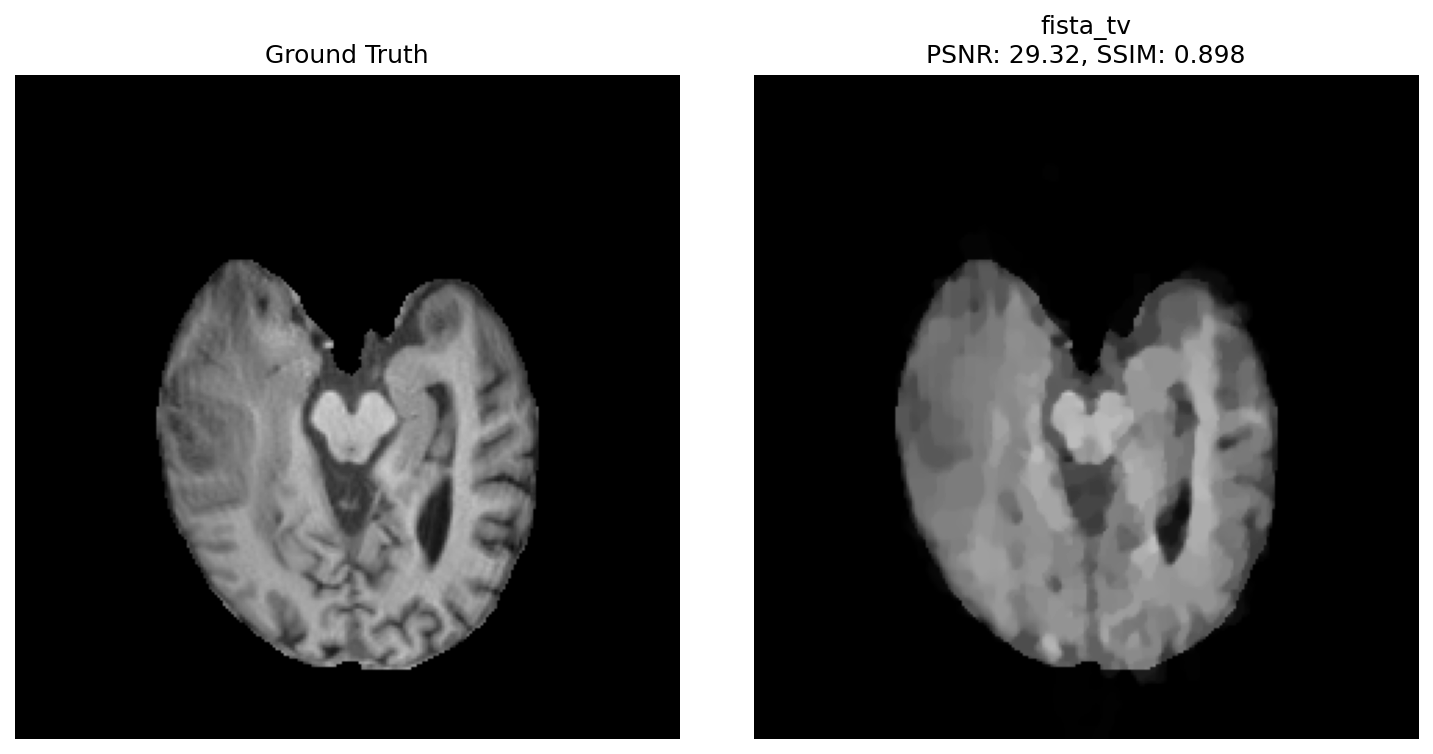
\includegraphics[trim={360pt 0 0 0}, clip,
        width=0.3\linewidth]{figs/fista_tv_batch0000.png} &
        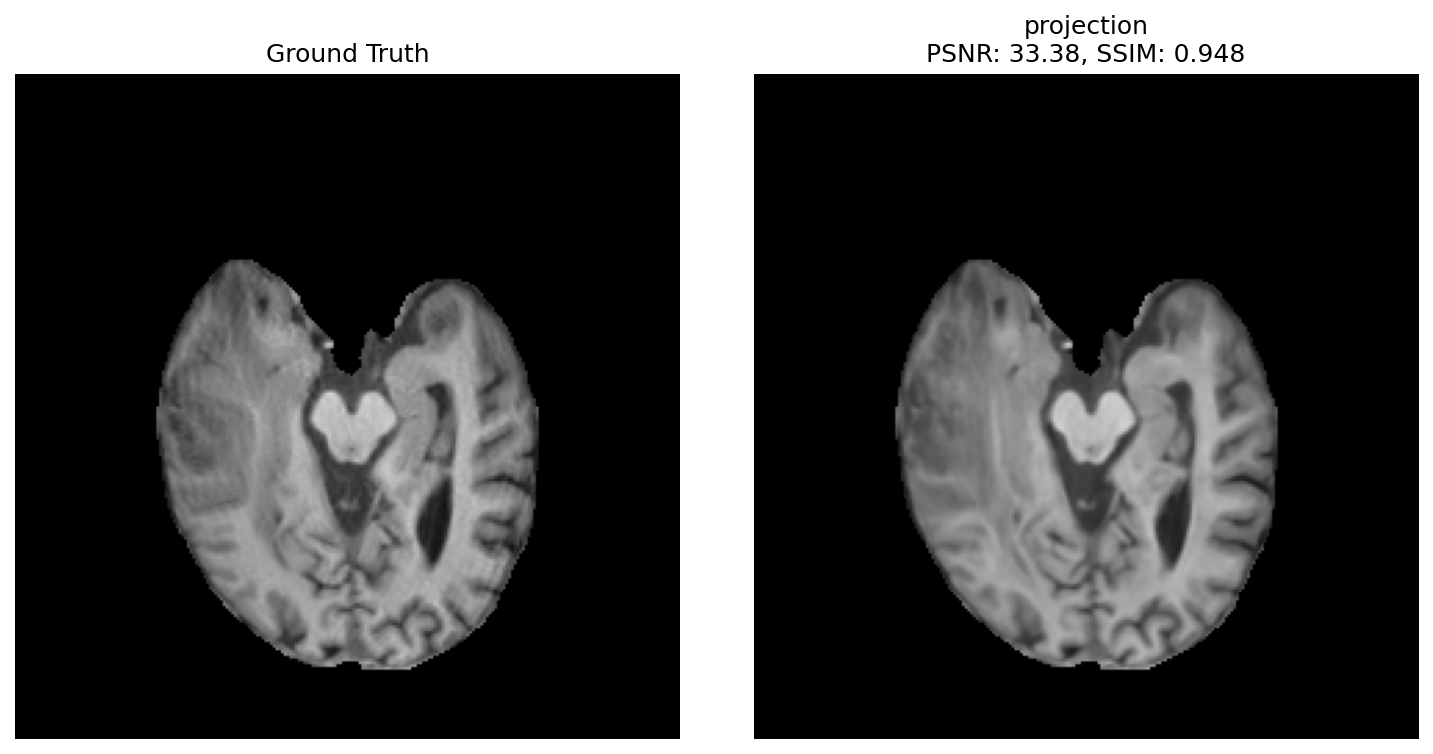
\includegraphics[trim={360pt 0 0 0}, clip,
        width=0.3\linewidth]{figs/projection_batch0000.png} &
        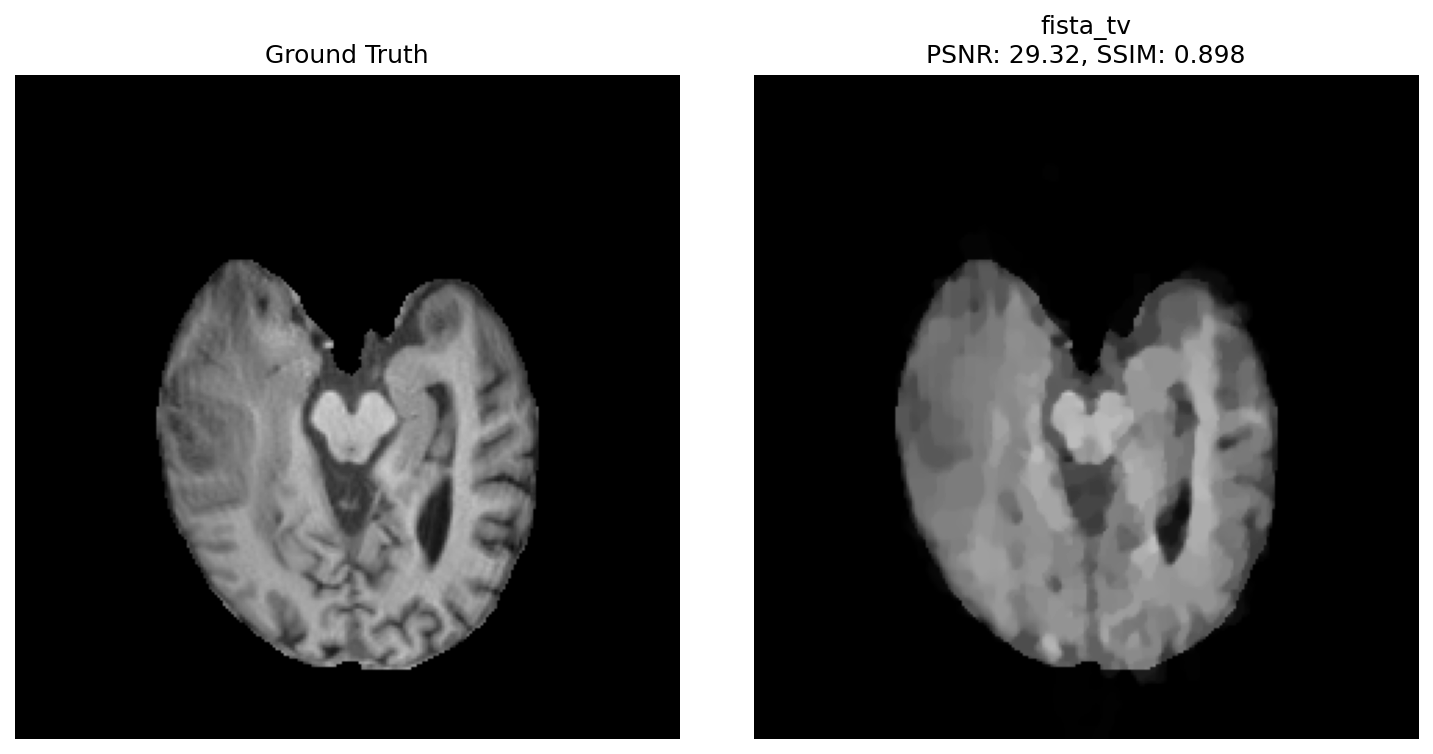
\includegraphics[trim={0 0 360pt 0}, clip,
        width=0.3\linewidth]{figs/fista_tv_batch0000.png} \\[2pt]
        % Row 2 - batch0002
        % 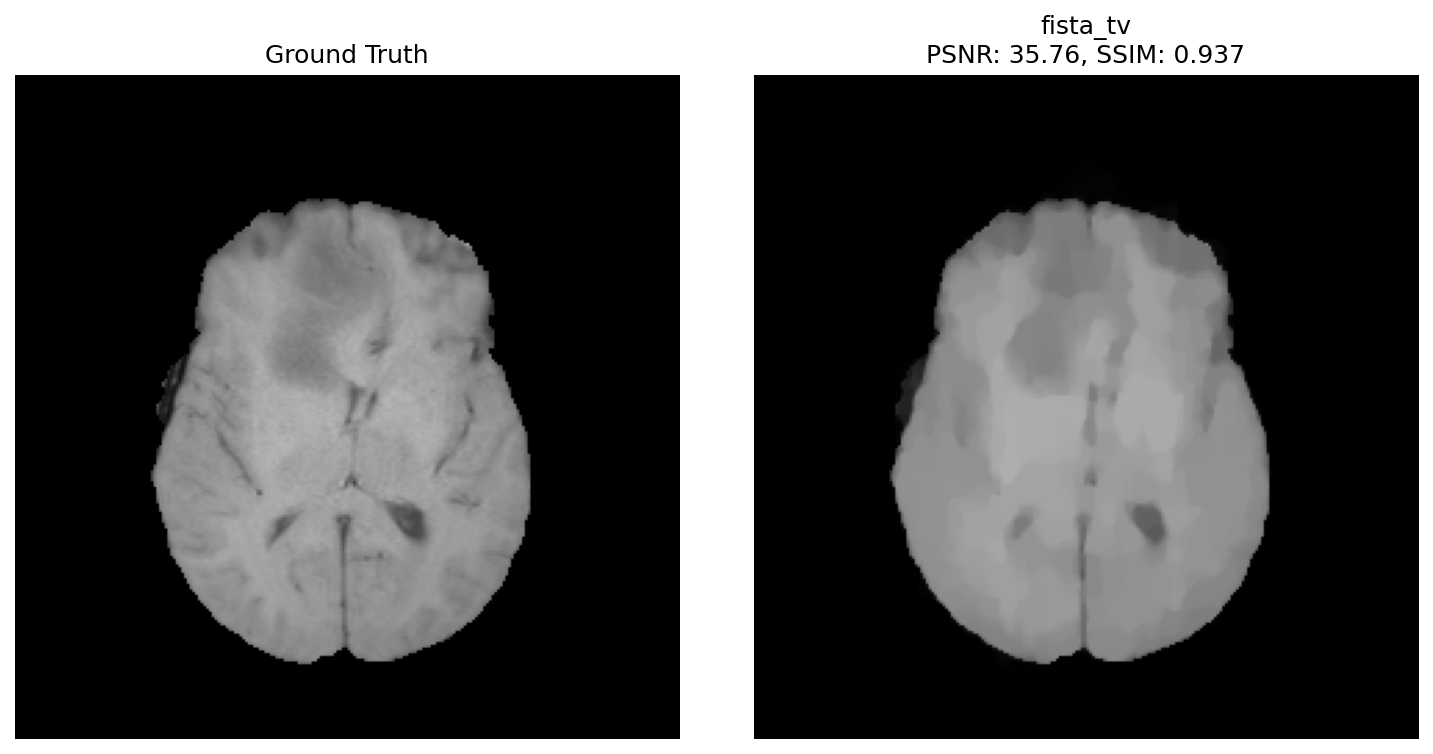
\includegraphics[trim={360pt 0 0 0}, clip,
        % width=0.3\linewidth]{figs/fista_tv_batch0002.png} &
        % 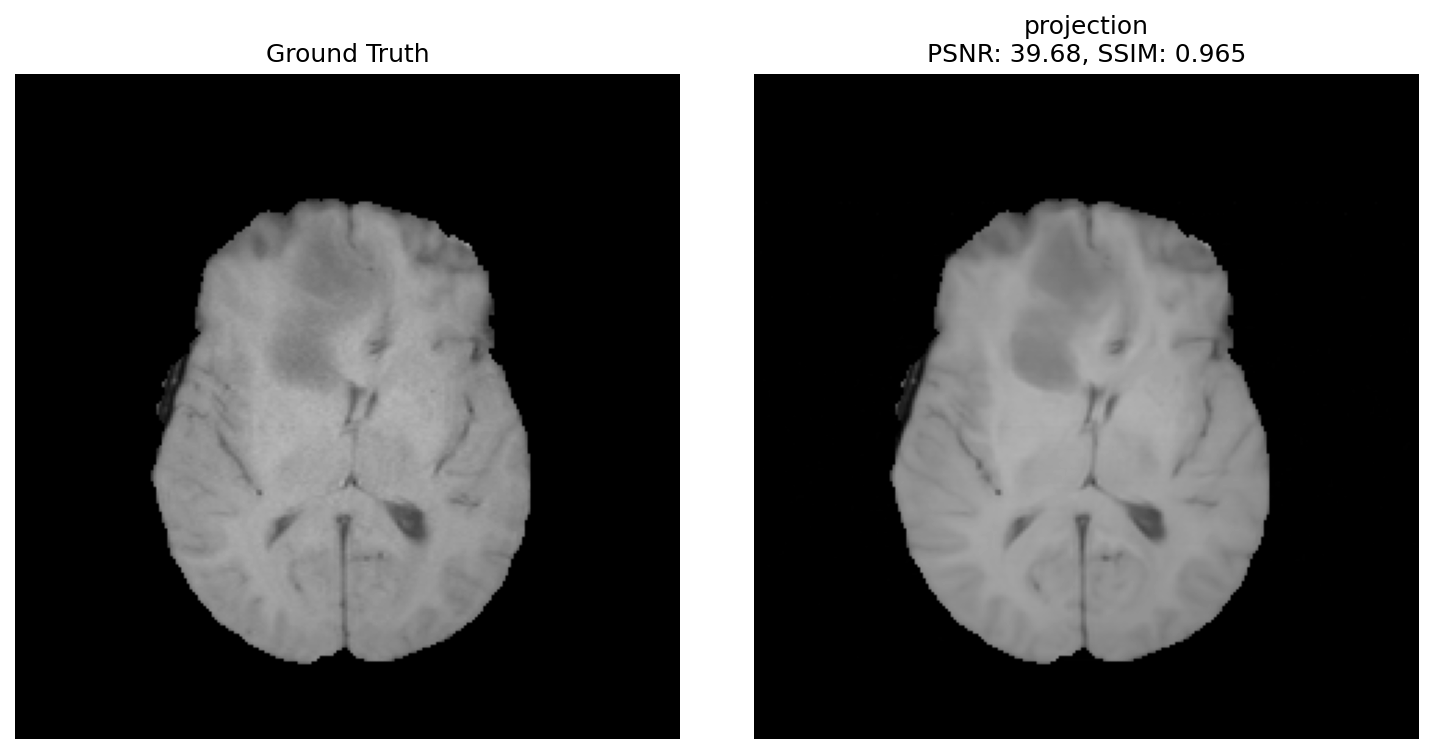
\includegraphics[trim={360pt 0 0 0}, clip,
        % width=0.3\linewidth]{figs/projection_batch0002.png} &
        % 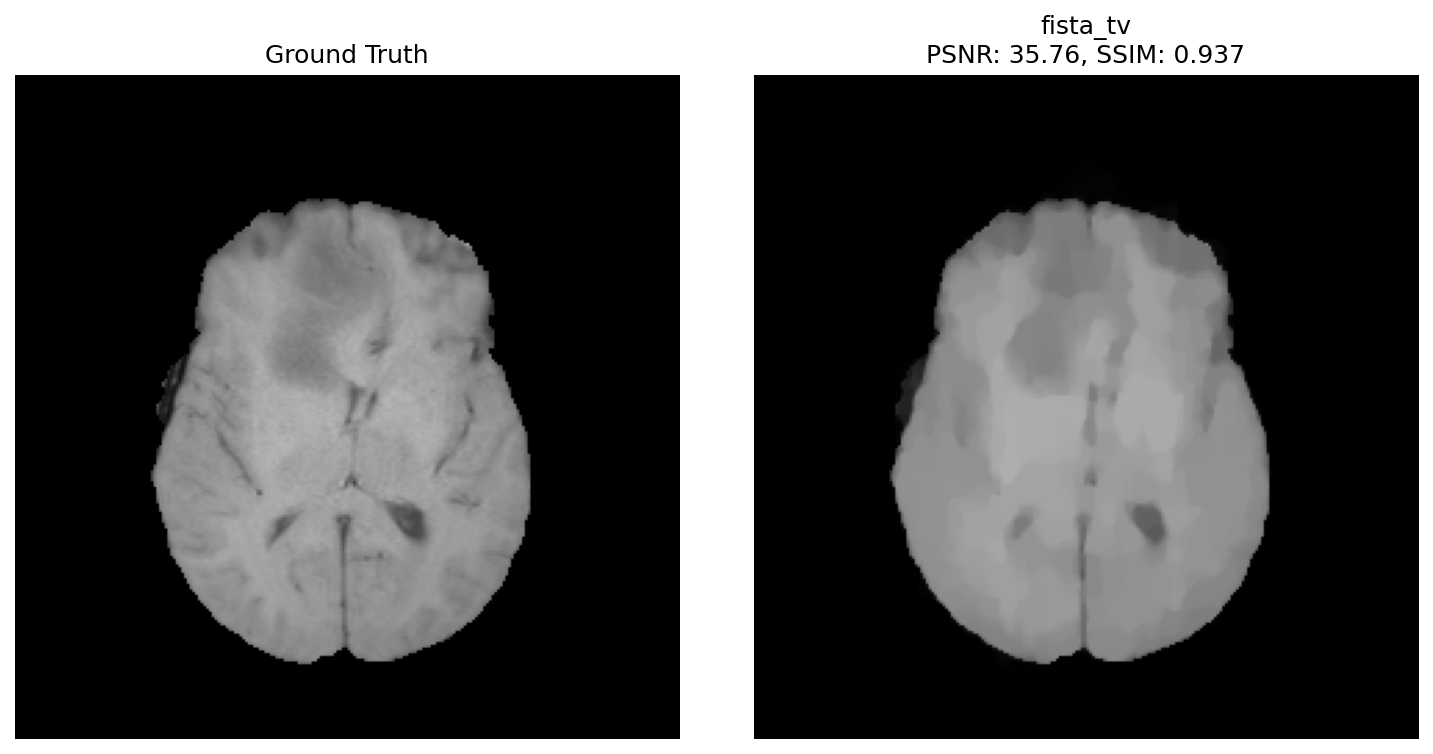
\includegraphics[trim={0 0 360pt 0}, clip,
        % width=0.3\linewidth]{figs/fista_tv_batch0002.png} \\[2pt]
        % Row 3 - batch0006
        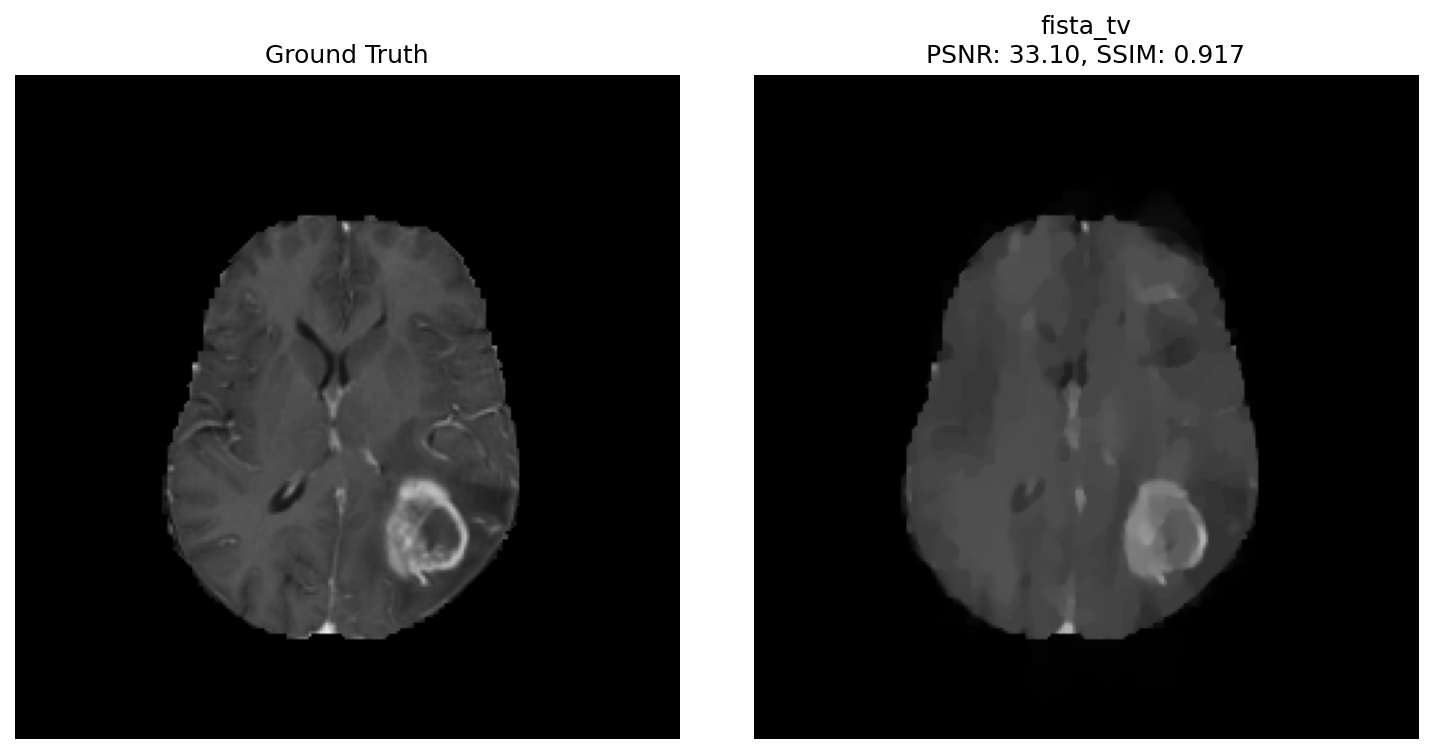
\includegraphics[trim={360pt 0 0 0}, clip,
        width=0.3\linewidth]{figs/fista_tv_batch0006.png} &
        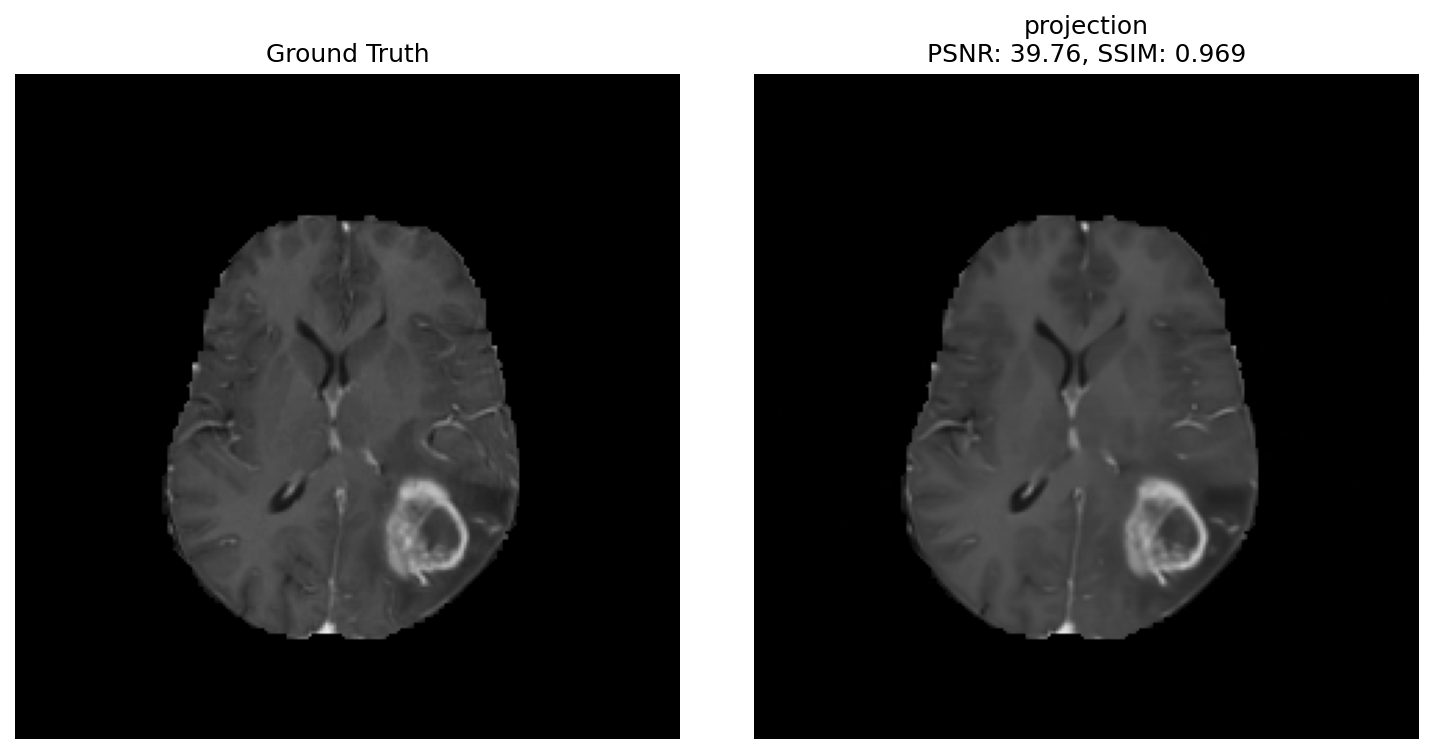
\includegraphics[trim={360pt 0 0 0}, clip,
        width=0.3\linewidth]{figs/projection_batch0006.png} &
        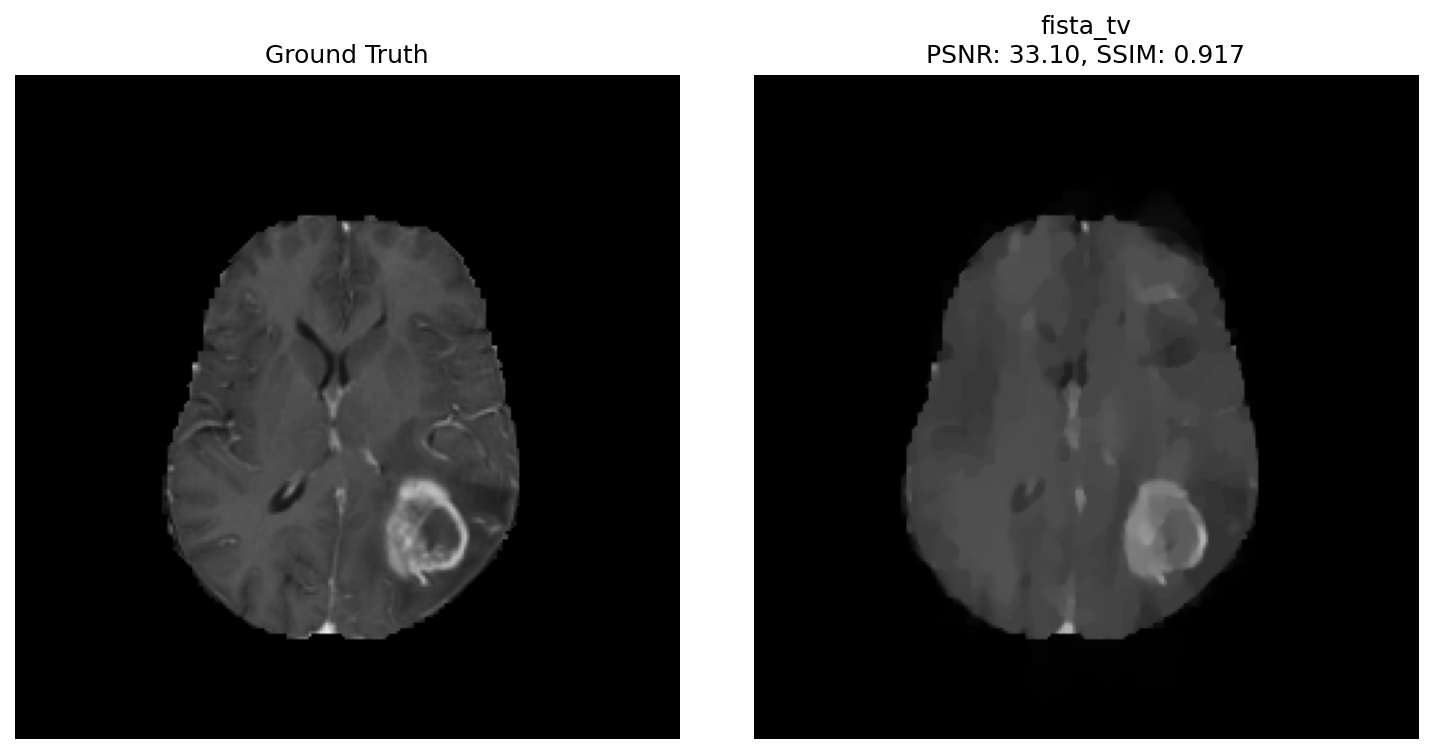
\includegraphics[trim={0 0 360pt 0}, clip,
        width=0.3\linewidth]{figs/fista_tv_batch0006.png}
    \end{tabular}
    \caption{\textbf{MRI 重建方法的视觉比较。}
        三个大脑 MRI 重建示例，展示了 FISTA-TV、
        测量
        一致性扩散方法（\textcite{song2022solving}），以及真实
        图像，这些图像来自 8 倍
        欠采样的 BraTS MRI 重建数据集。
        基于扩散的方法产生的重建结果更
        接近真实结构，与
        FISTA-TV 相比，后者可以被
        看出对真实
        图像中存在的精细细节进行了过度平滑。同
        时，在基于扩散的重建中，对真实
        图像的
        保真度（源于对
    测量一致性的适当强制执行）是惊人的。}
    \label{fig:mri-reconstruction-visual}
\end{figure}

\begin{table}[t]
    \centering
    \begin{tabular}{@{}lccc@{}}
        \toprule
        方法 & $24\times$ 加速 & $8\times$ 加速 & $4\times$ 加速 \\
        \midrule
        Cascade DenseNet & $23.39_{\pm 2.17}$ & $28.35_{\pm 2.30}$ &
        $30.97_{\pm 2.33}$ \\
        DuDoRNet & $18.46_{\pm 3.05}$ & $\bf 37.88_{\pm 3.03}$ &
        $30.53_{\pm 4.13}$ \\
        \textcite{song2020score} & $27.83_{\pm 2.73}$ & $35.04_{\pm
        2.11}$ & $37.55_{\pm 2.08}$ \\
        \textcite{NEURIPS2021_7d6044e9} & $28.80_{\pm 3.21}$ &
        $36.44_{\pm 2.28}$ & $38.76_{\pm 2.32}$ \\
        \textcite{song2022solving} & $\bf 29.42_{\pm 3.03}$ &
        $37.63_{\pm 2.70}$ & $\bf 39.91_{\pm 2.67}$ \\
        \bottomrule
    \end{tabular}
    \caption{\textbf{MRI 重建结果}，比较了在 BraTS MRI
        重建数据集上不同加速因子（$\cS$ 中傅里叶
        空间子采样的程度）下的测量匹配
        方法。报告了带有
        标准差的 PSNR 指标（越高越好）。
        Cascade DenseNet
        \cite{NEURIPS2019_1e48c442} 和 DuDoRNet \cite{9156506} 是在 8 倍加速
        级别下在成对样本上训练的监督
        基线。最后
        三种方法是使用
        测量一致性的基于扩散的方法。
    经 \textcite{song2022solving} 许可复制。}
    \label{tab:mri-reconstruction}
\end{table}

\section{使用成对数据和测量值的条件推断}
\label{sec:paired-data}
在许多实际应用中，我们既不知道感兴趣数据 $\x$ 的分布，
也不知道数据与数据的某些观测属性 $\y$ 之间的显式
关系。我们只有一个（大型的）成对样本集 $(\X, \Y) =
\{ (\x_1, \y_1), \ldots, (\x_N, \y_N) \}$，我们需要从中推断
数据分布以及一个对它们之间关系进行建模的映射：
\begin{equation}
    h: \x \mapsto \y.
\end{equation}

图像分类问题可以被视为这样一个
例子。在某种意义上，分类问题是为自然图像学习一个
（极度有损的）压缩编码器。例如，给定
图像 $\x$ 的一个随机样本，我们希望预测其最能关联 $\x$ 中内容的类别
标签 $\y$。我们知道，
与像素空间的维度相比，物体自然图像的分布是低维的。
从前面的章节中，我们
了解到，给定足够的样本，原则上，我们可以
通过学习到的压缩编码为 $\x$ 学习一个结构化的低维表征 $\z$：
\begin{equation}
    f: \x \mapsto \z.
\end{equation}
表征 $\z$ 也可以被视为 $\x$ 的一个学习到的（有损但
结构化的）代码。非常合理地假设，如果
类别分配 $\y$ 真正依赖于 $\x$ 的低维
结构，并且学习到的代码 $\z$ 真正反映了这种
结构，那么 $\y$ 和 $\z$ 可以变得高度相关，因此
它们的联合分布 $p(\z, \y)$ 应该是极度
低维的。因此，我们可以将两个期望的代码 $\y$
和 $\z$ 结合在一起，并尝试学习一个组合编码器：
\begin{equation}
    f: \x \mapsto (\z, \y)
\end{equation}
其中 $(\z, \y)$ 的联合分布是高度低维的。

根据我们在前面章节中的研究，映射 $f$ 通常被
学习为同一空间中的一系列压缩或去噪算子。
因此，为了利用这样一族操作，我们可以
引入一个辅助向量 $\vw$，它可以被视为类别标签 $\y$ 的初始
随机猜测。通过这种方式，我们可以学习一个压缩或去噪映射：
\begin{equation}\label{eq:classifier-with-class-token}
    f: (\x, \vw) \mapsto (\z, \y)
\end{equation}
在一个公共空间内。事实上，在用于
分类任务的 Transformer（例如 ViT）的训练中引入
辅助“类别标记 (class token)”的常见做法，可以被视为通过压缩给定（含噪）
样本 $(\x, \vw)$（的编码率）来学习这样
一个表征。如果数据 $\x$ 的分布
已经是一个（低维）高斯混合分布，文献
\cite{wright2008classification} 已经表明，通过直接最小化与给定样本相关的
{\em （有损）编码长度}，可以有效地进行分类。

\subsection{类条件图像生成}\label{sub:cfg}
虽然学习到的分类器允许我们将给定图像 $\x$ 分类到其
对应的类别，但我们通常希望通过
对学习到的自然图像分布进行采样，来生成给定类别的图像。在某种程度上，这可以被
视为图像分类的“逆”问题。令 $p_{\x}$ 表示
自然图像的分布，例如由扩散-去噪过程建模。
给定一个类别标签随机变量 $y \in [K]$ 及其
实现 $\nu$，例如
“苹果”，我们希望对条件分布 $p_{\x \mid
y}(\,\cdot\, \mid \nu)$ 进行采样以生成一张苹果的图像：
\begin{equation}
    \hat{\x} \sim p_{\x\mid \y}(\,\cdot\, \mid \vnu).
\end{equation}
我们称之为{\em 类条件图像生成}。

在 \Cref{sec:conditioned-decoding} 中，我们已经看到了如何使用
去噪-扩散范式，
在给定\textit{基于模型}的测量值 $\vy = h(\vx) + \vw$
（\Cref{eq:measurement-matching-observation}）的情况下，从后验 $p_{\vx \mid \vy}$ 中进行条件采样，最终得到了
DPS 算法（\Cref{alg:iterative_denoising_conditional_DPS}）。这
是一个强大的
框架，但它不适用于此处的类（或文本）条件图像
生成问题，因为由于解析建模的难解性，无法获得
观测值/属性 $y$ 的显式生成模型 $h$。在本节中，我们将
介绍将
条件采样扩展到此设定的技术。

因此，我们现在仅假设我们可以访问来自 $(\vx, y)$ 联合
分布的样本：
\begin{equation}
    (\vx, y) \sim p_{\vx, y}.
\end{equation}
与上一节一样，我们定义 $\vx_t = \alpha_t \vx + \sigma_t \vg$，
其中 $\vg \sim \cN(\Zero, \vI)$ 独立于 $(\vx, \vy)$，如
\Cref{ch:denoising} 中的 \Cref{eq:gen_additive_gaussian_noise_model} 所示，
并且我们将反复使用符号 $\vxi$ 来表示 $\vx$
和 $\vx_t$ 的实现。

本节重点介绍现代生成模型中条件采样的概念和算法基础。
有关各种应用中
实现问题的讨论，请参见 \Cref{ch:applications}、
\Cref{sec:cond_gen} 及后续小节。

\subsubsection{分类器引导：通过预训练分类器实现一致性}

% To proceed, we note that our development of conditional sampling under
% measurements $\vy = h(\vx) + \vw$ only explicitly used the
% forward model $h$ in making the DPS approximation
% \eqref{eq:conditional-posterior-measurementmatching-gaussian-case-dps-approx}.
回顾 \Cref{sec:conditioned-decoding}，
最优条件后验去噪器的以下分解
成立，
% In particular, the conditional posterior denoiser decomposition
% \eqref{eq:posterior-sampling-denoiser-decomposition} \textit{still
% holds in the
% paired data setting},
这是由于贝叶斯法则
以及在给定 $\vx$ 的情况下 $\vy$ 和 $\vx_t$ 的条件独立性（回顾
\Cref{fig:posterior-sampling-cds}）：
\begin{equation}\label{eq:conditional-denoising-mmse-denoiser-paired-data}
    \bE[ \vx \mid \vx_t=\vxi, y=\nu]
    =
    \bE[\vx \mid \vx_t=\vxi]
    + \frac{\sigma_t^2}{\alpha_t}
    \nabla_{\vxi}\log p_{y \mid \vx_t}(\nu\mid \vxi).
\end{equation}
换句话说，
无论显式观测模型 $\vy = h(\vx) + \vw$ 是否有效，
最优条件去噪器的表示
\eqref{eq:conditional-denoising-mmse-denoiser-paired-data} 都成立。
这意味着，如果我们能在成对数据
设定中学习到这样一个去噪器 \eqref{eq:conditional-denoising-mmse-denoiser-paired-data}，我们就可以遵循我们在
\Cref{ch:denoising} 中开发的去噪-扩散方法来执行类条件采样。

因此，一个自然的想法是直接使用参数为 $\theta_{\mathrm{c}}$ 的深度网络 $f_{\theta_{\mathrm{c}}}$ 来实现
\eqref{eq:conditional-denoising-mmse-denoiser-paired-data} 中的似然校正项，如
\Cref{eq:classifier-with-class-token} 所示：
\begin{equation}
    f_{\theta_{\mathrm{c}}} : (t, \vx_t) \mapsto \softmax(\vW_{\mathrm{head}}
    \vz(t, \vx_t)).
\end{equation}
该表达式将含噪输入
$\vx_t$ 的最终表征 $\vz(t, \vx_t)$
（它也依赖于
$\theta_{\mathrm{c}}$）与分类头 $\vW_{\mathrm{head}} \in \bR^{K
\times d}$ 结合起来，后者将
表征映射到 $K$ 个可能类别的概率分布上。
正如实践中常见的那样，它还将加噪过程中的时间 $t$ 作为
输入。
因此，通过适当的训练，它提供了对对数似然 $\log p_{y \mid \vx_t}$ 的近似，
并且对 $\log f_{\theta_{\mathrm{c}}}$ 关于其输入 $\vx_t$ 求导
允许对 \Cref{eq:conditional-denoising-mmse-denoiser-paired-data} 中的第二项进行近似：
\begin{equation}\label{eq:conditional-denoising-mmse-denoiser-paired-data-approx}
    \bar{\vx}_{\theta}^{\mathrm{naive}}(t, \vx_t, y)
    =
    \bar{\vx}_{\theta_{\mathrm{d}}}(t, \vx_t)
    + \frac{\sigma_t^2}{\alpha_t}
    \nabla_{\vx_t}
    \ip*{
        \log f_{\theta_{\mathrm{c}}}(t, \vx_t)
    }{
        \ve_{y}
    }
\end{equation}
其中，像往常一样，我们通过一个学习到的、参数为 $\theta_{\mathrm{d}}$ 的 $\vx_t$ 无条件去噪器来近似
\Cref{eq:conditional-denoising-mmse-denoiser-paired-data} 中的第一项，
并且我们记 $\ve_k$ ($k \in [K]$) 为 $\R^K$ 的第 $k$ 个标准基
向量（即第 $k$ 个位置为 1，其他位置为 0 的向量）。
读者应注意，条件去噪器 $\bar{\vx}_{\theta}$
需要两次独立的训练运行，并使用独立的损失：一次是针对
分类器参数 $\theta_{\mathrm{c}}$，使用分类
损失\footnote{在 \Cref{ch:applications} 中，我们详细回顾了训练此类分类器的过程。}，另一次是针对去噪器参数
$\theta_{\mathrm{d}}$，使用去噪损失。这种条件采样方法
在早期的扩散模型开创性工作中（特别是
\citet{Sohl-Dickstein2015} 和 \citet{song2020score} 的工作）就已经被认识到并用于执行条件采样。

然而，这种直接的方法有两个主要缺点（这就是为什么我们将其
标记为“朴素的”）。第一个缺点是，
根据经验，这样训练出来的深度网络分类器通常不能
提供足够强的引导信号（在
\Cref{eq:conditional-denoising-mmse-denoiser-paired-data} 中）以确保
生成的样本反映条件信息 $y$。这首先由 \citet{Dhariwal2021-hg} 强调，他们指出，在
类条件 ImageNet 生成的设定中，学习到的深度网络
分类器对于作为条件的类别 $y$ 的概率输出通常在
0.5 左右——大到足以成为主导类别，但不足以提供
强有力的引导信号——并且经检查，生成结果与
条件类别 $y$ 并不一致。\citet{Dhariwal2021-hg} 提出通过在朴素条件去噪器
\eqref{eq:conditional-denoising-mmse-denoiser-paired-data-approx} 的定义中
启发式地引入一个“逆温度”
超参数 $\gamma > 0$ 来解决这个问题，
并将由此产生的条件去噪器称为结合了\textbf{“分类器
引导”}
(CG)：
\begin{equation}\label{eq:conditional-denoising-mmse-denoiser-paired-data-approx-cg}
    \bar{\vx}_{\theta}^{\mathrm{CG}}(t, \vx_t, y)
    =
    \bar{\vx}_{\theta_{\mathrm{d}}}(t, \vx_t)
    + \gamma\frac{\sigma_t^2}{\alpha_t}
    \nabla_{\vx_t}
    \ip*{
        \log f_{\theta_{\mathrm{c}}}(t, \vx_t)
    }{
        \ve_{y}
    }
\end{equation}
其中 $\gamma = 1$ 的情况与
\eqref{eq:conditional-denoising-mmse-denoiser-paired-data-approx} 一致。

\citet{Dhariwal2021-hg} 发现设置 $\gamma > 1$ 在经验上表现
最好。
对此的一种可能解释如下：请注意，在\textit{真实}似然项
\Cref{eq:conditional-denoising-mmse-denoiser-paired-data} 的上下文中，
乘以 $\gamma$ 等价于给出
\begin{align}
    \gamma\frac{\sigma_t^2}{\alpha_t} \nabla_{\vxi}\log p_{\vy \mid
    \vx_t}(\vnu\mid
    \vxi)
    &=
    \frac{\sigma_t^2}{\alpha_t} \nabla_{\vxi}\log \left(
        p_{\vy \mid \vx_t}(\vnu\mid \vxi)^\gamma
    \right), %
\end{align}
这表明了参数 $\gamma$ 的自然解释，即对似然
$p_{\vy \mid \vx_t}$ 执行（逆）\textit{温度缩放}，如果我们考虑重归一化
分布
$ { p_{\vy \mid \vx_t}(\vnu\mid \vxi)^\gamma } / { \int p_{\vy \mid
    \vx_t}(\vnu'\mid
\vxi)^\gamma \odif \vnu' } $，这是精确的。
然而，请注意，在 \Cref{eq:conditional-denoising-mmse-denoiser-paired-data} 的上下文中，这\textit{不是}一个严格的解释，
因为
梯度是关于 $\vxi$ 计算的，并且温度缩放分布中的归一化常数通常是 $\vxi$ 的函数。
相反，参数 $\gamma$ 应该简单地被理解为放大深度网络分类器输出概率
$f_{\theta_{\mathrm{c}}}(t, \vx_t)$ 的较大值，\textit{相对于}较小的值，
这有效地放大了在深度
network $f$ 在 $K$ 个类别中为其分配了最大的概率。

\subsubsection{通过无分类器引导的简化与改进}

尽管如此，分类器引导（classifier guidance）并没有解决朴素方法的第二个关键缺点：除了无条件去噪器 $\bar{\vx}_{\theta_{\mathrm{d}}}$ 之外，还必须训练一个辅助分类器 $f_{\theta_{\mathrm{c}}}$，这既繁琐又浪费。因为我们无法直接调整预训练的分类器，它需要能够在噪声输入 $\vx_t$ 上良好工作，并结合其他基于经验动机的架构修改。
特别是，\citet{Dhariwal2021-hg} 发现必须 \textit{显式地设计实现分类器的深度网络架构，使其与去噪器的架构相匹配}。

此外，纯粹从实用的角度来看——为了从生成的采样器中获得最佳性能——基于分类器引导的采样的最佳性能配置，进一步偏离了我们上面提出的理想化且概念上合理的框架。
为了获得最佳性能，\citet{Dhariwal2021-hg} 发现有必要将类别标签 $y$ 作为额外输入提供给去噪器 $\bar{\vx}_{\theta_{\mathrm{d}}}$。因此，由 \citet{Dhariwal2021-hg} 推导出的理想化分类器引导去噪器 \eqref{eq:conditional-denoising-mmse-denoiser-paired-data-approx-cg}（正如我们上面从条件后验去噪器分解 \eqref{eq:conditional-denoising-mmse-denoiser-paired-data} 中推导的那样），并不能完全反映实践中性能最好的去噪器——这种去噪器实际上结合了给定 $y$ 时 $\vx_t$ 的 \textit{条件} 去噪器，以及来自辅助分类器的额外引导信号！

这种基于经验动机的现状，促使 \citet{Ho2022-ry} 在随后的工作中提出了一种在经验上更具实用性的方法，称为 \textbf{无分类器引导（classifier-free guidance, CFG）}。他们没有将条件去噪器 \eqref{eq:conditional-denoising-mmse-denoiser-paired-data} 表示为 $\vx_t$ 的无条件去噪器与对数似然校正项的加权和（可能像分类器引导中那样修改了权重），而是接受了 \citet{Dhariwal2021-hg} 的实验结果所证明的、训练给定 $y$ 时 $\vx_t$ 的条件去噪器的明显必要性，并将对数似然梯度项替换为该条件去噪器与给定 $\vx_t$ 时 $\vx$ 的 \textit{无条件} 去噪器的正确加权和。\footnote{尽管如此，\textcite{Ho2022-ry} 实际上建议使用与我们在此处展示的不同的权重，这是基于 \textcite{Dhariwal2021-hg} 启发式地将 \eqref{eq:conditional-denoising-mmse-denoiser-paired-data} 中的无条件去噪器替换为条件去噪器这一事实。事实上，我们在此推导和展示的权重反映了现代实践，特别是被用于最先进的扩散模型中，例如 Stable Diffusion 3.5 \cite{DBLP:conf/icml/EsserKBEMSLLSBP24}。}

\paragraph{推导无分类器引导。} 为了理解这种结构是如何产生的，我们从分类器引导去噪器 $\bar{\vx}_{\theta}^{\mathrm{CG}}$ 的“理想化”版本开始，该版本在 \eqref{eq:conditional-denoising-mmse-denoiser-paired-data-approx-cg} 中定义，对于该版本，去噪器 $\bar{\vx}_{\theta_{\mathrm{d}}}$ 和分类器 $f_{\theta_{\mathrm{c}}}$ 通过 \eqref{eq:conditional-denoising-mmse-denoiser-paired-data} 完美地逼近了它们的目标：
\begin{equation}\label{eq:conditional-denoising-mmse-denoiser-paired-data-exact-cg}
    \bar{\vx}_{\theta}^{\mathrm{CG,\,ideal}}(t, \vxi, \nu)
    =
    \bE[\vx \mid \vx_t=\vxi]
    + \gamma\frac{\sigma_t^2}{\alpha_t}
    \nabla_{\vxi}\log p_{y \mid \vx_t}(\nu\mid \vxi).
\end{equation}
然后我们使用贝叶斯法则，其形式为
\begin{equation}
    \log p_{y \mid \vx_t}
    =
    \log p_{\vx_t \mid y} + \log p_{y} - \log p_{\vx_t},
\end{equation}
结合 Tweedie 公式（\Cref{thm:tweedie}，如 \Cref{eq:gen_tweedie} 中所修改）在得分函数和去噪器之间进行转换，得到
\begin{align*}
    \bar{\vx}_{\theta}^{\mathrm{CG,\,ideal}}(t, \vxi, \nu)
    &=
    \frac{1}{\alpha_t} \vxi
    + (1-\gamma) \frac{\sigma_t^2}{\alpha_t}
    \nabla_{\vxi}\log p_{\vx_t}(\vxi)
    + \gamma \frac{\sigma_t^2}{\alpha_t}
    \nabla_{\vxi}\log p_{\vx_t \mid y}(\vxi \mid \nu)
    \\
    &=
    (1 - \gamma) \bE[\vx \mid \vx_t=\vxi]
    +
    \gamma \bE[\vx \mid \vx_t=\vxi, y=\nu],
    \labelthis\label{eq:ideal-cfg-denoiser}
\end{align*}
在最后一行中，我们应用了 \Cref{eq:conditional-denoising-conditioning-order-irrelevant}。
现在，\Cref{eq:ideal-cfg-denoiser} 提出了一种自然的近似策略：如前所述，我们将给定 $\vx_t$ 时 $\vx$ 的已学习无条件去噪器，与给定 $\vx_t$ 和 $y$ 时 $\vx$ 的已学习 \textit{条件} 去噪器结合起来。

然而，遵循 \textcite{Ho2022-ry} 以及训练深度网络去噪器的常见实践，标准的做法是使用 \textit{同一个} 深度网络来同时表示条件去噪器和无条件去噪器，方法是引入一个额外的标签（我们将用 $\varnothing$ 表示）来指代“无条件”情况。
这导出了 CFG 去噪器的形式：
\begin{equation}\label{eq:conditional-denoising-mmse-denoiser-paired-data-approx-cfg}
    \bar{\vx}_{\theta}^{\mathrm{CFG}}(t, \vx_t, y)
    =
    (1 - \gamma) \bar{\vx}_{\theta}(t, \vx_t, \varnothing)
    +
    \gamma \bar{\vx}_{\theta}(t, \vx_t, y).
\end{equation}
为了训练一个用于无分类器引导采样的去噪器 $\bar{\vx}_{\theta}(t, \vx_t, y^+)$，其中 $y^+ \in
\set{1, \dots, K, \varnothing}$，我们的过程与 \Cref{alg:learning_denoiser} 中的无条件训练过程几乎完全相同，但有两个修改：
\begin{enumerate}
    \item 当我们从数据集中采样时，我们采样一个数据对 $(\vx,
        y)$，而不仅仅是一个样本 $\vx$。
    \item 每次我们从数据集中采样一个数据对时，我们通过以下方式采样增广标签 $y^+$：
        \begin{equation}
            y^+ =
            \begin{cases}
                \varnothing & \text{概率为 } p_{\mathrm{uncond}}; \\
                y & \text{否则}.
            \end{cases}
        \end{equation}
        这里，$p_{\mathrm{uncond}} \in [0, 1]$ 是一个新的超参数。这可以被视为一种 dropout 形式 \cite{srivastava2014dropout}。
\end{enumerate}
通过这种方式，我们训练了一个适用于无分类器引导采样的条件去噪器。我们在 \Cref{alg:iterative_denoising_conditional_CFG} 中总结了带有无分类器引导的类别条件采样的整体采样过程。

\begin{algorithm}
    \caption{使用分类数据和类别条件去噪器进行条件采样。}
    \label{alg:iterative_denoising_conditional_CFG}
    \begin{algorithmic}[1]
        \Require{用于采样的有序时间步列表 \(0 \leq t_{0} < \cdots
        < t_{L} \leq T\)。}
        \Require{作为条件的类别标签 $\nu \in \set{1, \dots, K}$。}
        \Require{针对 $p_{\vx \mid y}$ 和 $p_{\vx}$ 的去噪器 \(\bar{\vx}_{\theta} \colon
                \{t_{\ell}\}_{\ell = 1}^{L} \times \R^{D} \times
                \set{1, \dots, K,
            \varnothing} \to \R^{D}\)（对于 $p_{\vx}$ 输入 $\varnothing$）。}
        \Require{尺度和噪声水平函数 \(\alpha, \sigma
        \colon \{t_{\ell}\}_{\ell = 0}^{L} \to \R_{\geq 0}\)。}
        \Require{引导强度 $\gamma \geq 0$（为了性能通常首选 $\gamma > 1$）。}
        \Ensure{一个样本 \(\hat{\vx}\)，近似服从 \(p_{\vx
                \mid y}(\,\cdot\,
        \mid \nu)\)。}
        \Function{DDIMSamplerConditionalCFG}{$\bar{\vx}_{\theta}, \nu, \gamma,
        (t_{\ell})_{\ell = 0}^{L}$}
        \State{初始化 \(\hat{\vx}_{t_{L}} \sim\) \(\vx_{t_{L}}\) 的近似分布（VP \(\implies
        \dNorm(\vzero, \vI)\)，VE \(\implies \dNorm(\vzero, t_{L}^{2}\vI)\)）。}
        \For{\(\ell = L, L - 1, \dots, 1\)}
        \State{计算
            \begin{equation*}
                \hat{\vx}_{t_{\ell - 1}} \doteq \frac{\sigma_{t_{\ell
                - 1}}}{\sigma_{t_{\ell}}}\hat{\vx}_{t_{\ell}} +
                \bp{\alpha_{t_{\ell
                    - 1}} - \frac{\sigma_{t_{\ell
                - 1}}}{\sigma_{t_{\ell}}}\alpha_{t_{\ell}}}\bigl(
                    (1 - \gamma) \bar{\vx}_{\theta}(t_{\ell},
                    \hat{\vx}_{t_{\ell}}, \varnothing)
                    + \gamma \bar{\vx}_{\theta}(t_{\ell},
                    \hat{\vx}_{t_{\ell}}, \nu)
                \bigr)
            \end{equation*}
        }
        \EndFor
        \State{\Return{\(\hat{\vx}_{t_{0}}\)}}
        \EndFunction
    \end{algorithmic}
\end{algorithm}

\textcite{Ho2022-ry} 报告了带有无分类器引导的类别条件图像生成具有强大的经验性能，并且它已成为最大规模的实用扩散模型（如 Stable Diffusion \cite{rombach2022high} 及其衍生模型）的支柱。

\paragraph{无分类器引导促进学习什么样的去噪器？}
正如我们所见，无分类器引导的推导相当不透明且基于经验动机，几乎没有提供关于其强大性能背后机制的深入见解。
许多理论工作试图解决这个问题 \cite{Bradley2024-jg,Li2025-li,Wu2024-js}。
它们为整体 CFG 方法的某些部分提供了理论解释——该方法本身涵盖了去噪器的参数化和训练，以及采样时引导强度的配置和性能。
下面，遵循本书贯穿始终的主题，我们将在高斯混合模型数据分布和去噪器的简化设置中给出一种解释。
首先，我们考虑 \textit{CFG 的作用}：较大的权重 $\gamma \gg 1$ 会促进什么？

% \yima{Please make messages that the example below try to convey some
% what more modular. Probably break it into two related parts?}
\begin{example}\label{example:denoising-gaussian-mixture-cfg}
    让我们回顾一下我们在 \Cref{example:denoising_gaussian_mixture} 中研究的低秩高斯混合数据生成过程（特别是 \Cref{eq:MoG1} 中的形式）。给定 $K \in \bN$ 个类别，我们假设
    \begin{equation}\label{eq:MoG1-ch6}
        \vx \sim \frac{1}{K}\sum_{k = 1}^{K}\dNorm(\vzero,
        \vU_{k}\vU_{k}^{\top}),
    \end{equation}
    其中每个 \(\vU_{k} \in \O(D, P) \subseteq \R^{D \times P}\) 是一个具有正交列的矩阵，且 $P \ll D$。
    此外，我们假设类别标签 $y \in [K]$ 是 $\vx$ 的确定性函数，将样本映射到其对应的混合成分。
    我们考虑在 \Cref{ch:denoising} 中研究的简单噪声过程 \eqref{eq:additive_gaussian_noise_model}，因此对于所有 $t \in [0, T]$，有 $\vx_t = \vx + t \vg$，其中 $\vg \sim \cN(\Zero,
    \vI)$。

    应用 \Cref{example:denoising_gaussian_mixture} 中的分析（以及随后对低秩情况的分析，最终得出 \Cref{eq:gmm_lowrank_denoiser}），我们得到对于每个 $\nu \in [K]$ 的类别条件最优去噪器为
    \begin{equation}\label{eq:gmm_lowrank_denoiser-ch6-classcond}
        \bE[ \vx \mid \vx_t = \vxi, y = \nu ]
        = \frac{1}{1 + t^{2}}
        \vU_{\nu}\vU_{\nu}^{\top}\vxi
    \end{equation}
    而对于最优无条件去噪器，我们得到
    \begin{equation}\label{eq:gmm_lowrank_denoiser-ch6-uncond}
        \bE[ \vx \mid \vx_t = \vxi ]
        = \frac{1}{1 + t^{2}}\sum_{k =
        1}^{K}\frac{\exp\rp{\frac{1}{2t^{2}(1 +
        t^{2})}\norm{\vU_{k}^{\top}\vxi}_{2}^{2}}}{\sum_{i =
            1}^{K}\exp\rp{\frac{1}{2t^{2}(1 +
        t^{2})}\norm{\vU_{i}^{\top}\vxi}_{2}^{2}}}\vU_{k}\vU_{k}^{\top}\vxi.
    \end{equation}
    因此，我们可以将引导强度为 $\gamma > 1$ 的 CFG 去噪器表示为
    \begin{equation}\label{eq:cfg-denoiser-mog-low-rank}
        \begin{split}
            \bar{\vx}^{\mathrm{CFG,\,ideal}}(t, \vx_t, y)
            =
            \frac{1}{1 + t^{2}}
            \Biggl(
                &(1 - \gamma)
                \sum_{k = 1}^{K}\frac{\exp\rp{\frac{1}{2t^{2}(1
                + t^{2})}\norm{\vU_{k}^{\top}\vx_t}_{2}^{2}}}{\sum_{i
                    = 1}^{K}\exp\rp{\frac{1}{2t^{2}(1
                                +
                t^{2})}\norm{\vU_{i}^{\top}\vx_t}_{2}^{2}}}\vU_{k}\vU_{k}^{\top}
                \\
                &\qquad+
                \gamma
                \vU_{y}\vU_{y}^{\top}
            \Biggr)
            \vx_t.
        \end{split}
    \end{equation}

    该去噪器具有简单、可解释的形式：
    \begin{enumerate}
        \item 第一项对应于 \textit{无条件去噪器}，它对信号 $\vx_t$ 进行去噪，去噪目标是与每个子空间相关的去噪器的平均值，其权重取决于 $\vx_t$ 与每个子空间的相关程度。
        \item 第二项对应于 \textit{条件去噪器}，它简单地使用条件类别的去噪器进行去噪。
    \end{enumerate}

    CFG 方案对这两个去噪器进行平均。
    这种平均的效果可以从以下重构中看出
    \begin{equation}\label{eq:cfg-denoiser-mog-low-rank-2}
        \begin{split}
            \bar{\vx}^{\mathrm{CFG,\,ideal}}(t, \vx_t, y)
            =
            \frac{1}{1 + t^{2}}
            &\Biggl(
                \left[\gamma + (1 - \gamma)
                    \frac{\exp\rp{\frac{1}{2t^{2}(1
                    + t^{2})}\norm{\vU_{y}^{\top}\vx_t}_{2}^{2}}}{\sum_{i
                        = 1}^{K}\exp\rp{\frac{1}{2t^{2}(1
                    + t^{2})}\norm{\vU_{i}^{\top}\vx_t}_{2}^{2}}}
                \right]
                \vU_{y}\vU_{y}^{\top}
                \\
                &\quad+
                (1 - \gamma)
                \sum_{k \neq y}\frac{\exp\rp{\frac{1}{2t^{2}(1
                + t^{2})}\norm{\vU_{k}^{\top}\vx_t}_{2}^{2}}}{\sum_{i
                    = 1}^{K}\exp\rp{\frac{1}{2t^{2}(1
                                +
                t^{2})}\norm{\vU_{i}^{\top}\vx_t}_{2}^{2}}}\vU_{k}\vU_{k}^{\top}
            \Biggr)
            \vx_t,
        \end{split}
    \end{equation}
    其中我们将条件去噪器与对 $k \in [K]$ 求和中对应的 $k=y$ 项结合起来。
    我们有
    \begin{equation}
        \sum_{k=1}^K
        \frac{\exp\rp{\frac{1}{2t^{2}(1
        + t^{2})}\norm{\vU_{k}^{\top}\vx_t}_{2}^{2}}}{\sum_{i
            = 1}^{K}\exp\rp{\frac{1}{2t^{2}(1
        + t^{2})}\norm{\vU_{i}^{\top}\vx_t}_{2}^{2}}}
        = 1,
    \end{equation}
    并且每个加数都是非负的，因此其上界也为 $1$。
    因此，我们可以得出 \Cref{eq:cfg-denoiser-mog-low-rank-2} 中各项的两种状态（regimes）：
    \begin{enumerate}
        \item \textbf{高相关状态：} 在这种情况下，假设噪声输入 $\vx_t$ 与其中一个子空间 $\vU_y$ 高度相关。如果 $\vx_t$ 与 $\vU_y$ 高度相关，那么无条件去噪器中对应于 $k=y$ 加数的归一化权重接近于 $1$。
            那么
            \begin{equation}
                \gamma + (1 - \gamma)
                \frac{\exp\rp{\frac{1}{2t^{2}(1
                + t^{2})}\norm{\vU_{y}^{\top}\vx_t}_{2}^{2}}}{\sum_{i
                    = 1}^{K}\exp\rp{\frac{1}{2t^{2}(1
                + t^{2})}\norm{\vU_{i}^{\top}\vx_t}_{2}^{2}}}
                \approx 1,
            \end{equation}
            所有其他权重必然接近于零，并且 CFG 去噪器近似等于与条件类别 $y$ 相关的去噪器。

            这意味着：\textit{如果 CFG 去噪器的输入与其中一个类别子空间高度相关，则该去噪器近似等于相应的类别条件去噪器}！因此，我们期望 CFG 去噪采样器能够收敛。
        \item \textbf{低相关状态：} 相反，如果 $\vx_t$ 与 $\vU_y$ \textit{不} 高度相关（例如因为 $t$ 很大），那么无条件去噪器中对应于 $k=y$ 加数的归一化权重接近于 $0$。结果，
            \begin{equation}
                \gamma + (1 - \gamma)
                \frac{\exp\rp{\frac{1}{2t^{2}(1
                + t^{2})}\norm{\vU_{y}^{\top}\vx_t}_{2}^{2}}}{\sum_{i
                    = 1}^{K}\exp\rp{\frac{1}{2t^{2}(1
                + t^{2})}\norm{\vU_{i}^{\top}\vx_t}_{2}^{2}}}
                \approx \gamma,
            \end{equation}
            因此引导强度 $\gamma \gg 1$ 会在与 $y$ 相关的去噪器上放置一个很大的正权重。

            同时，在 \Cref{eq:cfg-denoiser-mog-low-rank-2} 的第二项中，任何与 $\vx_t$ 高度相关的类别 $k \neq y$ 都会从 $1 - \gamma$ 系数中获得一个很大的 \textit{负} 权重。
            这同时产生了一种效果，使得去噪后的信号与条件类别 $y$ 的相关性大大增加，并使其与前一次迭代（即去噪前的迭代）呈负相关。

            换句话说，\textit{CFG 引导迭代去噪过程朝向条件类别，并远离前一次迭代}，这是一种不同于纯条件采样（即 $\gamma = 1$ 的情况）的动力学。
    \end{enumerate}
\end{example}

\Cref{example:denoising-gaussian-mixture-cfg} 表明，在高斯混合设置中，CFG 去噪器提供了对条件类别的强烈偏置，同时在噪声水平 $t$ 较小时保留了局部正确性（因此保证了采样的收敛性）。
这暗示了为什么在实践中发现较大的权重 $\gamma \gg 1$ 是必不可少的。

接下来，下面的例子将展示在存在低维结构的情况下，对去噪器 \textit{参数化} 的深入见解，同样是在高斯混合模型中。

\begin{example}\label{example:denoising-gaussian-mixture-cfg-parameterization}
    再次考虑在 \Cref{example:denoising-gaussian-mixture-cfg} 中研究的高斯混合模型：
    \begin{equation}
        \vx \sim \frac{1}{K}\sum_{k = 1}^{K}\dNorm(\vzero,
        \vU_{k}\vU_{k}^{\top}),
    \end{equation}
    其中每个 \(\vU_{k} \in \O(D, P) \subseteq \R^{D \times P}\) 是一个具有正交列的矩阵，且 $P \ll D$。
    类别标签 $y \in [K]$ 是 $\vx$ 的确定性函数，将样本映射到其对应的混合成分。
    对于该分布，并且再次在 \Cref{ch:denoising} 中研究的简单噪声过程 \eqref{eq:additive_gaussian_noise_model} 下（其中对于所有 $t \in [0, T]$ 有 $\vx_t = \vx + t \vg$，且 $\vg \sim \cN(\Zero,
    \vI)$），我们在 \Cref{example:denoising-gaussian-mixture-cfg} 中看到理想的 CFG 去噪器具有以下形式
    \begin{equation}\label{eq:cfg-denoiser-mog-low-rank-3}
        \begin{split}
            \bar{\vx}^{\mathrm{CFG,\,ideal}}(t, \vx_t, y)
            =
            \frac{1}{1 + t^{2}}
            \Biggl(
                &(1 - \gamma)
                \sum_{k = 1}^{K}\frac{\exp\rp{\frac{1}{2t^{2}(1
                + t^{2})}\norm{\vU_{k}^{\top}\vx_t}_{2}^{2}}}{\sum_{i
                    = 1}^{K}\exp\rp{\frac{1}{2t^{2}(1
                                +
                t^{2})}\norm{\vU_{i}^{\top}\vx_t}_{2}^{2}}}\vU_{k}\vU_{k}^{\top}
                \\
                &\qquad+
                \gamma
                \vU_{y}\vU_{y}^{\top}
            \Biggr)
            \vx_t.
        \end{split}
    \end{equation}

    % We now perform a further analysis of the form of this guided denoiser in
    % order to make some inferences about the role of CFG.
    % % Many of these insights
    % % will be relevant to \textit{general} data distributions with
    % low-dimensional
    % % geometric structure, as well.
    % First, notice that the CFG denoiser \eqref{eq:cfg-denoiser-mog-low-rank-3}
    % takes a simple form in the setting where $\vx_t$ correlates
    % significantly more
    % strongly with a single subspace $\vU_y$ than any other $\vU_{y'}$. Indeed,
    % because the ratio of weights in the class-conditional denoiser is given by
    % \begin{equation}
    %     \frac{
    %         \exp\rp{\frac{1}{2t^{2}(1 +
    %         t^{2})}\norm{\vU_{y}^{\top}\vx_t}_{2}^{2}}
    %     }{
    %         \exp\rp{\frac{1}{2t^{2}(1 +
    %         t^{2})}\norm{\vU_{y'}^{\top}\vx_t}_{2}^{2}}
    %     }
    %     =
    %     \exp\rp{
    %         \frac{1}{2t^{2}(1 + t^{2})}\left(
    %             \norm{\vU_{y}^{\top}\vx_t}_{2}^{2}
    %             -
    %             \norm{\vU_{y'}^{\top}\vx_t}_{2}^{2}
    %         \right)
    %     },
    % \end{equation}
    % a large separation between the correlation of $\vx_t$ with
    % $\vU_{y}$ and other
    % subspaces $\vU_{y'}$ implies that the sum over $k$ concentrates
    % on the $k=y$
    % summand, giving that \textit{the CFG denoiser remains equal to the
    % class-conditioned denoiser}. Moreover, when $t \approx 0$, the
    % magnitude of
    % any such gap is amplified in the exponential, making this
    % concentration on the
    % $k=y$ summand even stronger. In particular, for small times $t$
    % (i.e., near to
    % the support of the data distribution), CFG denoising is no different from
    % standard class-conditional denoising---implying that it will
    % converge stably
    % once it has reached such a configuration.
    % Thus, the empirical benefits of CFG should be due to its behavior in cases
    % where $\vx_t$ is not unambiguously from a single class.

    现在我们考虑参数化一个可学习的去噪器 $\vx_{\theta}^{\mathrm{CFG}}$ 以表示最优去噪器 \eqref{eq:cfg-denoiser-mog-low-rank-3} 的问题。
    % Here, it may initially seem that the setting of classification
    % of a mixture
    % distribution is too much of a special case relative to learning
    % practical data
    % distributions, as the ideal denoiser
    % \eqref{eq:cfg-denoiser-mog-low-rank-3} has
    % in this setting the simple form of a \textit{hard assignment} of the
    % noisy signal $\vx_t$ to the (denoiser associated to) the subspace $\vU_y$
    % corresponding to the true class label $y$ of $\vx$, averaged with the
    % \textit{soft assignment} denoiser associated to all subspaces
    % $\vU_k$, with
    % weights given by the correlations of $\vx_t$ with these
    % different subspaces.
    % However, we can extract a more general form for the
    % class-conditional denoiser
然而，我们可以为类别条件去噪器提取一个更一般的形式
    % 在这个与使用高斯混合分布的几何结构进行实际参数化相关的例子中，
    % 高斯混合分布的几何结构，
    % 实际上
    % 类似于现实世界数据中常见的几何结构。
    % 更准确地说，
    为了易于处理，我们增加了一个与子空间 $\vU_k$ 彼此“可区分”相关的额外假设，这在实践中是很自然的：具体而言，我们假设对于任意一对索引 $k, k' \in
    [K]$ 且 $k \neq k'$，我们可以找到一组 $K$ 个非零方向 $\vv_{k} \in \bR^D$，使得
    \begin{equation}
        \vU_{k}\vU_{k}^\top \vv_k = \vv_k, \quad
        \vU_{k'}\vU_{k'}^\top \vv_k = \Zero, \enspace k' \neq k.
    \end{equation}
    这是一个比简单的可区分性稍强的假设，但需要注意的是，它并不算过于严格：例如，它仍然允许子空间 $\vU_{k}$ 之间存在显著的相关性。\footnote{更一般地，这个假设可以自然地表述为子空间 $\vU_{[K]}$ 之间的\textit{不相干条件}（incoherence condition），这在压缩感知理论中很常见 \cite{Wright-Ma-2022}。}

    这些向量 $\vv_k$ 可以被视为类别标签 $y \in [K]$ 的\textit{嵌入}（embeddings），我们可以使用它们来定义一个更一般的算子，该算子可以同时表示无条件和类条件去噪器。
    更准确地说，考虑映射
    \begin{equation}\label{eq:mog-conditional-denoising-unified-operator}
        (\vx_t, \vv) \mapsto
        \sum_{k = 1}^{K}\frac{
            \exp\rp{\frac{1}{2t^{2}(1
            + t^{2})} \abs{\vx_t^\top \vU_k \vU_k^\top \vv}}
        }
        {
            \sum_{i
            = 1}^{K}\exp\rp{\frac{1}{2t^{2}(1
            + t^{2})}\abs{\vx_t^\top \vU_i \vU_i^\top \vv}}
        }
        \vU_{k}\vU_{k}^{\top}\vx_t.
    \end{equation}
    那么，如果我们将 $\vv = \vx_t$ 代入算子
    \eqref{eq:mog-conditional-denoising-unified-operator}，我们会得到一个与
    \eqref{eq:gmm_lowrank_denoiser-ch6-uncond} 中第一项成正比的结果，对应于 $\vx_t$ 的最优无条件去噪器。
    另一方面，
    如果我们对于某个 $y \in [K]$ 代入 $\vv = \vv_y$，根据嵌入向量 $\vv_k$ 的构造，我们得到
    \begin{eqnarray}
        &&\sum_{k = 1}^{K}
        \frac{
            \exp\rp{\frac{1}{2t^{2}(1
            + t^{2})}\abs{\vx_t^\top \vU_k \vU_k^\top \vv_y}}
        }
        {
            \sum_{i
            = 1}^{K}\exp\rp{\frac{1}{2t^{2}(1
            + t^{2})}\abs{\vx_t^\top \vU_i \vU_i^\top \vv_y}}
        }
        \vU_{k}\vU_{k}^{\top}\vx_t \nonumber \\
        &=&
        \frac{
            \exp\rp{\frac{1}{2t^{2}(1
            + t^{2})}\abs{\vx_t^\top \vv_y}}
        }
        {
            \exp\rp{\frac{1}{2t^{2}(1
            + t^{2})}\abs{\vx_t^\top \vv_y}}
            + K-1
        }
        \vU_{y}\vU_{y}^{\top}\vx_t
        \\
        && +
        \sum_{k \neq y}
        \frac{
            1
        }
        {
            \exp\rp{\frac{1}{2t^{2}(1
            + t^{2})}\abs{\vx_t^\top \vv_y}}
            + K-1
        }
        \vU_{k}\vU_{k}^{\top}\vx_t.
    \end{eqnarray}

    我们的目标是进一步简化上述表达式。
    为此，回想一下，当使用该去噪器进行采样时，我们有
    $\vx_t = \vx + t \vg$，其中 $y$ 表示 $\vx$ 的标签。
    换句话说，在给定 $y$ 的条件下，我们有 $\vx_t = \vU_y \vz
    + t \vg$，其中 $\vz$ 是一个独立的 $P$ 维高斯噪声向量，具有零均值和单位协方差。
    我们有
    \begin{align*}
        \abs*{\vx_t^\top \vv_y}
        &=
        \abs*{\ip{\vU_y \vz}{\vv_y} + t \ip{\vg}{\vv_y}}
        \\
        &=
        \abs*{\ip{\vz}{\vU_y^\top \vv_y} + t \ip{\vg}{\vv_y}}.
    \end{align*}
    因为 $\vz$ 和 $\vg$ 是具有单位协方差矩阵的独立高斯随机变量，根据高斯分布的\textit{旋转不变性}（见 \cite{Vershynin2018-br}），可得
    \begin{align*}
        \abs*{\vx_t^\top \vv_y}
        &\equid
        \abs*{\norm{\vU_y^\top \vv_y}_2 z + t\norm{\vv_y}_2 g}
        \\
        &=
        \abs*{\norm{\vv_y}_2 z + t\norm{\vv_y}_2 g},
    \end{align*}
    其中 $z$ 和 $g$ 是独立的\textit{标量} $\cN(0, 1)$ 随机变量，$\equid$ 表示依分布相等（随机变量具有相同的分布）。
    上面的第二行由 $\vv_y$ 的定义得出。
    现在，由独立性可知，随机变量 $z + tg \sim \cN(0, (1 + t^2))$。
    然后利用众所周知的结果，即如果 $g
    \sim \cN(0, 1)$，则 $\bE[\abs{g}] = \sqrt{2/\pi}$，我们可以得出结论
    \begin{equation*}
        \bE\left[
            \abs*{\vx_t^\top \vv_y}
        \right]
        =
        \sqrt{(2/\pi) (1 + t^2)} \norm{\vv_y}_2.
    \end{equation*}
    在实践中，根据高斯集中不等式（再次参见 \cite{Vershynin2018-br}），量 $ \abs*{\vx_t^\top \vv_y}$ \textit{以极大概率}接近其期望。
    另一方面，通过类似的推理，我们有
    \begin{equation*}
        \bE\left[
            \norm*{\vx_t}_2^2
        \right]
        =
        P + t^2 D,
    \end{equation*}
    高斯分布的性质再次表明，$\norm{\vx_t}_2$ 将以极大概率集中在 $\sqrt{P + t^2 D}$ 附近。
    因此，对嵌入 $\vv_y$ 进行重新归一化，使其与 $\vx_t$ 的点积具有相同的尺度是合理的：定义
    \begin{equation*}
        \vv_{t, y} = \frac{(P + t^2 D)}{\sqrt{(2/\pi)(1 + t^2)}}
        \frac{\vv_y}{\norm{\vv_y}_2}
    \end{equation*}
    作为归一化后的嵌入，我们之前的论证意味着
    \begin{equation*}
        \abs*{\vx_t^\top \vv_{t,y}}
        \approx
        (P + t^2 D)
    \end{equation*}
    以极大概率成立。
    将注意力转回我们的起点，即在 $(\vx_t,
    \vv_y)$ 处计算的 \eqref{eq:mog-conditional-denoising-unified-operator} 及其随后的简化，对于“softmax”的参数，我们有
    \begin{equation*}
        {\frac{1}{2t^{2}(1 + t^{2})}\abs{\vx_t^\top \vv_y}}
        \approx
        \frac{P + t^2 D}{2t^{2}(1 + t^{2})}
    \end{equation*}
    关于 $\vx_t$ 以极大概率成立。
    因此，如果 $t$ 是有界的且子空间维度 $P$ 足够大，\footnote{例如，只需考虑一个大规模的渐近状态，其中 $P, D \to \infty$ 且它们的比率
        $P/D$ 收敛到一个固定常数。在这种情况下，子空间的\textit{纵横比}是固定的，而它们的大小趋于无穷大，这可以作为某些离散化现象的模型（例如，将固定场景采样为图像，像素数量趋于无穷大）。}
    % 那么根据前面的表达式，
    % 如果
    % 子空间维度
    % $P$ 足够大——对于 $t \approx 0$，我们有
    % $\norm{\vx_t}_2$ 接近于
    % $\sqrt{P}$，根据测度集中现象\footnote{这是
    %     少数几个\textit{维度灾难的福音}（blessings of dimensionality）之一——参见
    % \textcite{Wright-Ma-2022}。}。那么
    % 根据上一段的论证，在这种状态下，对于
    % $\vx_t$ 的\textit{几乎所有}实现，
    以下近似以极大概率成立：
    \begin{equation}
        \sum_{k = 1}^{K}
        \frac{
            \exp\rp{\frac{1}{2t^{2}(1
            + t^{2})}\vx_t^\top \vU_k \vU_k^\top \vv_y}
        }
        {
            \sum_{i
            = 1}^{K}\exp\rp{\frac{1}{2t^{2}(1
            + t^{2})}\vx_t^\top \vU_i \vU_i^\top \vv_y}
        }
        \vU_{k}\vU_{k}^{\top}\vx_t
        \approx
        \vU_{y}\vU_{y}^{\top}\vx_t.
    \end{equation}
    换言之，\textbf{在类别嵌入 $\vv_{t, y}$ 处计算算子
        \eqref{eq:mog-conditional-denoising-unified-operator} 即可得到 $y$ 的类条件去噪器！}
    % 这个论证表明，算子
    % \eqref{eq:mog-conditional-denoising-unified-operator} 以
    % 极大概率
    % \textit{等于最优类条件去噪器
    %     \eqref{eq:gmm_lowrank_denoiser-ch6-classcond}（对于 $y$）
    % 当 $\vv = \vv_y$ 时}！直观地说，在小噪声水平 $t \approx
    % 0$ 时——对应于去噪过程中强化结构的部分——
    % 将给定类别 $y$ 的嵌入代入算子
    % \eqref{eq:mog-conditional-denoising-unified-operator} 的第二个参数
    % 会使得关于 $\vx_t$ 的结果函数很好地近似最优
    % 类条件去噪器
    % \eqref{eq:gmm_lowrank_denoiser-ch6-classcond}（对于
    % $y$）。

    因此，算子族
    \eqref{eq:mog-conditional-denoising-unified-operator}
    提供了一种统一的方法，\textit{在单个“网络”内}参数化 $\vx$ 的最优去噪器中的组成算子。
    更准确地说，只需将输入为 $(\vx_t,
    \vx_t)$ 的 \eqref{eq:mog-conditional-denoising-unified-operator} 实例的输出与输入为 $(\vx_t, \vv_{t, y})$ 的实例的输出相加即可。
    所得算子是关于 $(t, \vx_t, y)$ 的函数，在计算上，子空间
    $(\vU_k)_{k=1}^K$ 和嵌入 $y \mapsto \vv_{t, y}$ 成为其可学习参数。
\end{example}

\Cref{example:denoising-gaussian-mixture-cfg-parameterization} 表明，在 $\vx$ 具有不相干分量的低秩高斯混合数据分布的特殊情况下，形式为
\begin{equation}\label{eq:operator-for-parameterizing-cfg-denoiser-mog}
    (\vx_t, \vv) \mapsto
    \sum_{k = 1}^{K}\frac{
        \exp\rp{\frac{1}{2t^{2}(1
        + t^{2})}\vx_t^\top \vU_k \vU_k^\top \vv}
    }
    {
        \sum_{i
        = 1}^{K}\exp\rp{\frac{1}{2t^{2}(1
        + t^{2})}\vx_t^\top \vU_i \vU_i^\top \vv}
    }
    \vU_{k}\vU_{k}^{\top}\vx_t
\end{equation}
的算子提供了一类足够丰富的算子，以便在使用无分类器引导时，参数化 $\vx$ 的噪声观测值 $\vx_t$ 的理想去噪器。
% 其中一个网络将用于同时表示
% $\vx_t$ 的无条件和类条件去噪器。
对于此类算子，
辅助输入 $\vv$ 可以取为 $\vx_t$ 或类别标签的合适嵌入 $y \mapsto \vv_y$，以实现这样的去噪器——如示例所示，理想去噪器是此类算子的加权和，其权重源自引导强度 $\gamma>1$。

基于 \Cref{ch:deep-networks} 中的框架（该框架开发了适合将更一般的数据分布转换为结构化表示的深度网络架构，并以低秩高斯混合模型作为基元），我们很自然地会设想，类型为
\eqref{eq:operator-for-parameterizing-cfg-denoiser-mog} 的算子可以用于一般数据分布 $\vx$ 的去噪器中，前提是这些分布具有彼此足够可区分（例如，不相干）的低维几何结构分量。
下一节将证明情况确实如此。

\subsection{基于字幕条件的图像生成}\label{sub:text-cond}
在 \Cref{sub:cfg} 中，我们已经在概念上看到了如何设置去噪器以与\textit{无分类器引导}（classifier-free guidance）结合使用，这是通过扩散-去噪范式执行条件采样的主要实用方法。
% 我们在类条件采样的特殊情况下实例化了这一点，其中
% 条件信号 $y$ 是一个标量。
简而言之，此类去噪器将噪声数据 $\vx_t$ 以及条件信号 $\vy$ 或“空输入” $\varnothing$ 作为输入，这决定了去噪器应执行\textit{无条件去噪}还是\textit{条件去噪}（以 $\vy$ 为条件）。

鉴于这种设计，最重要的实际问题是\textit{如何将这一算子族实现为神经网络？}
一种被称为“交叉注意力”（cross attention）的在经验上取得成功的神经网络层设计（我们将在适当的时候介绍）为这个问题提供了一个实用的答案。然而，在此之前，还有几个更基本的问题需要理清：
\begin{enumerate}
    \item \textit{输入模态不匹配}：在最有趣的实际应用中，数据 $\vx$ 和条件信号 $\vy$
        \textit{并不位于可直接比较的空间中}，尽管它们共享许多潜在的结构关系。例如，我们在
        \Cref{sub:cfg} 中的类别标签 $y$ 的情况下看到了这一点。更一般地说，可以考虑图像 $\vx$ 的自然语言描述 $\vy$（称为“字幕”），其中 $\vy$ 将对应于不同字母表中的字符序列。
    \item \textit{参数化与灵活性}：在输入模态问题的下游，存在一个基本问题，即网络是否可以使用相同的基本架构来处理不同的模态，或者是否需要针对每种模态进行非常精确的调整。
        % 使用通用架构是更可取的，因为它允许
        % 使用\textit{迁移学习}的可能性，其中
    \item \textit{训练}：这涉及使用成对样本 $(\vx, \vy)$ 来训练和部署条件去噪器的正确方法。
        设计空间是巨大的：可以想象应用我们在
        \Cref{ch:lossy-compression,ch:consistent-representations} 中开发的各种特定于模态的编码器-解码器架构，以及各种组合中的不同去噪主干。这里的关键问题是\textit{表达能力}（获得最佳的条件去噪性能）；\textit{效率}（获得单位训练数据的最佳性能）；以及\textit{稳定性}（保证训练过程快速收敛而不崩溃）。
\end{enumerate}

我们将在下面详细讨论这三个问题，提供有关如何探索设计空间的指导，并在可能的情况下提供通用的建议。

\subsubsection{模态无关的输入嵌入}

尽管在一般的成对数据设置中我们不知道 $\vx$ 和 $\vy$ 之间的精确关系，但在所有感兴趣的实际设置中，它们具有显著的相关性。例如，当条件信号 $\vy$ 是用自然语言描述图像 $\vx$ 的“字幕”时，很容易想象人类艺术家能够仅凭高质量的字幕就画出 $\vx$ 的准确草图。
在我们的概率设置中，量化这些“相关性”的一种自然方法是使用互信息，我们之前在
\Cref{ch:lossy-compression}（\Cref{eq:information-entropy}）中看到过：
\begin{equation}\label{eq:mutual-info-ch7}
    I(\vx; \vy) = h(\vx) - h(\vx \mid \vy).
\end{equation}
互信息 \eqref{eq:mutual-info-ch7} 是一个纯粹的信息论量，不依赖于 $\vx$ 和 $\vy$ 的特定模态方面。
因此，它为学习任一输入 $\vx$、$\vy$ 的有用表征提供了一个自然的准则：人们只需寻求学习（例如对于 $\vx$）一个保留互信息的表征 $\vz = f(\vx)$，使得
$I(\vz; \vy) \approx I(\vx; \vy)$。
也就是说：
\begin{equation}\label{eq:infomax-x-abstract}
    \text{学习} \enspace \vz = f(\vx) \enspace \text{使得} \enspace I(\vz;
    \vy) \approx I(\vx; \vy).
\end{equation}
实际上，我们在这里可以更具规定性。对于确定性的编码器 $f$（与我们在
\Cref{ch:lossy-compression,ch:consistent-representations} 中研究的所有情况相匹配），信息论中一个被称为\textit{数据处理不等式}（data processing inequality）的基本结果告诉我们，用 $f$ 处理 $\vx$ 以产生 $\vz = f(\vx)$ 会以一种可预测的方式改变互信息：\textit{它只会减少互信息}。
\begin{theorem}[数据处理不等式]\label{thm:dpi}
    考虑随机变量 $\vy, \vx, \vz$，其定义使得在给定 $\vx$ 的条件下，$\vz$ 独立于 $\vy$。\footnote{换句话说，这些随机变量形成了一个马尔可夫链 $\vy \to \vx \to \vz$。} 那么\textit{数据处理不等式}成立：
    \begin{equation}\label{eq:dpi-ch7}
        I(\vx; \vy) \geq I(\vz; \vy).
    \end{equation}
    \begin{proof}
        考虑 $\vy$ 和 $(\vx, \vz)$ 之间的互信息 $I(\vy; \vx, \vz)$。因为在给定 $\vx$ 的条件下 $\vz$ 独立于 $\vy$，我们有
        \begin{equation*}
            h(\vy \mid \vx, \vz) = h(\vy \mid \vx),
        \end{equation*}
        因此 $I(\vy; \vx, \vz) = I(\vy; \vx)$。同时，根据贝叶斯法则，我们有
        \begin{equation*}
            p_{\vy \mid \vx, \vz} = p_{\vy \mid \vz}
            % \frac{p_{\vx \mid \vy, \vz}}{p_{\vx \mid \vz}},
            \frac{p_{\vy, \vx, \vz}}{p_{\vy, \vz} p_{\vx \mid \vz}},
        \end{equation*}
        根据条件微分熵的定义，这意味着
        \begin{equation*}
            I(\vy; \vx, \vz) =
            I(\vy; \vz)
            - \bE_{\vx, \vy, \vz}\left[ \log \left(
                    % \frac{p_{\vx \mid \vz}}{p_{\vx \mid \vy, \vz}}
                    \frac{p_{\vx \mid \vz} p_{\vy, \vz}}{p_{\vy, \vx, \vz}}
            \right)\right].
        \end{equation*}
        将詹森不等式（Jensen's inequality）应用于上一行的期望即可得出该结论，因为 $\log$ 是一个凹函数（并且互信息是对称的，即 $I(\vx; \vy) = I(\vy; \vx)$）。
    \end{proof}
\end{theorem}

对于确定性编码器 $f$，在给定 $\vx$ 的条件下，$\vz = f(\vx)$ 总是独立于 $\vy$。
因此，数据处理不等式提出了以下寻找编码器 $f$ 的计算过程：\textit{寻求最大化表征与条件信号之间的互信息}。
\Cref{eq:infomax-x-abstract} 进而引出目标
\begin{equation}\label{eq:infomax-x}
    \max_{f}\, I(f(\vx); \vy).
\end{equation}
这被称为 \textit{Infomax 原理} \cite{infomax}，它可以追溯到表征学习的最早时期。

\paragraph{应用 Infomax 原理的计算考量。}

在思考如何应用（抽象的）Infomax 原理 \eqref{eq:infomax-x} 来学习表征时，有两个关键的概念性问题需要牢记。首先，通常在计算上很难估计互信息，而互信息构成了
\eqref{eq:infomax-x} 中的目标。
正如我们在 \Cref{ch:lossy-compression} 中引入互信息时在率失真和有损编码的背景下所讨论的那样，即使当 $\vx$ 和 $\vy$ 是低维的并且微分熵接近 $-\infty$ 时，互信息也可以被松弛以保持良好的定义（例如，通过与我们在
\Cref{ch:lossy-compression,ch:deep-networks,ch:consistent-representations} 中研究的高斯率衰减函数相联系）。
此外，经验表明，这种松弛在实践中具有非最坏情况的统计特性，正如我们在
\Cref{ch:lossy-compression} 的实验中所看到的那样；并且这些近似的准确性可以通过增量处理来提高，正如我们在 \Cref{ch:deep-networks} 中所看到的那样。
这使得像 \Cref{eq:infomax-x} 这样的准则成为学习成对数据 $(\vx, \vy)$ 表征的极佳基础。

需要牢记的第二个问题是，为了使目标 \eqref{eq:infomax-x} 成为学习 $f$ 的合理准则，必须以特定方式对 $f$ 本身进行参数化，和/或对表征 $f(\vx)$ 进行一些额外的结构约束。事实上，如果 $f$ 完全不受约束，\eqref{eq:infomax-x} 就会存在简单的平凡解，这些解并不对应于有用的表征：例如，只需取 $f(\vx) = \vx$ 为恒等映射即可！
在 \Cref{ch:consistent-representations} 中讨论自编码和闭环转录时，我们讨论了构建表征空间的原则性技术；其中许多技术可以应用于我们目前的联合嵌入设置中，我们将在本节后面转向实际实现时进一步详细说明这一点。

\paragraph{基于 Infomax 原理的联合嵌入。}

现在，仍然存在 $(\vx, \vy)$ 的\textit{联合}表征问题。再次应用数据处理不等式，对于产生 $\vy$ 表征的另一个编码器 $g$，我们得到
\begin{equation*}
    I(\vx; \vy) \geq I(f(\vx); \vy) \geq I(f(\vx); g(\vy)).
\end{equation*}
联合目标
\begin{equation}\label{eq:infomax-x-y}
    \max_{f, g}\, I(f(\vx); g(\vy))
\end{equation}
则是 Infomax 原理的一个有充分根据的推论。

为了设计编码器 $f$ 和 $g$，回想一下我们通过在
\Cref{example:denoising-gaussian-mixture-cfg-parameterization} 中的工作获得的直觉。在那里，我们看到在 $\vx$ 的高斯混合模型的情况下，条件信号 $y$ 标识了哪个特定的混合分量生成了观测值，通过将类别标签 $y$ 适当地嵌入到与数据 $\vx$ \textit{相同的空间}中，可以构建一个灵活的去噪器架构。
更准确地说，这样的嵌入 $\vu_y \in \R^D$ 允许在通过 $\vu_y^\top
\vU_{\vx}$ 与 $\vx \in \R^{D}$ 的嵌入 $\vU_{\vx}$（通常是一个矩阵）相关联时，仅“挑选出”与分布的正确混合分量相关的嵌入。
究竟如何设计这些层以用于在更复杂的非线性高维数据上训练的神经网络，是一个具有挑战性的问题，我们将在下面更详细地探讨。但一个必要条件是明确的：嵌入
$f$ 和 $g$ 应该将它们的输入映射到一个\textit{公共嵌入空间}（例如 $\R^d$），以促进在执行条件采样时的下游比较。
这引出了目标
\begin{equation}\label{eq:infomax-joint}
    \max_{f : \R^{D_{\vx}} \to \R^{d}, g: \R^{D_{\vy}} \to \R^d}\,
    I(f(\vx); g(\vy)).
\end{equation}

下一步是实例化 \eqref{eq:infomax-joint} 中互信息的一个合适的、计算上方便的松弛，以便用于大规模数据集。
\subsubsection{学习联合嵌入的实用方案：CLIP}

针对成对数据学习联合嵌入的一个具体且极具影响力的实现是对比语言-图像预训练（Contrastive Language-Image Pre-training, CLIP）方法 \cite{radford2021learning}。
以从数据集 $\mathcal{D}$ 中采样的图像-文本对 $[(\x_i, \y_i)]_{i=1}^N$ 为例，其中 $\x_i$ 是图像，$\y_i$ 是文本标题。
CLIP 训练了两个编码器——图像编码器 $f_{\theta}(\x)$ 和文本编码器 $g_{\plainphi}(\y)$——将成对样本映射到一个共享的 $d$ 维单位球面上（即 $\|f_{\theta}(\x_i)\|_2 = 1$ 且 $\|g_{\plainphi}(\y_i)\|_2 = 1$）。
为了实现这一点，我们可以采用一个简单的对称交叉熵损失，使匹配对 $(f_{\theta}(\x_i),g_{\plainphi}(\y_i))$ 的余弦相似度更接近，同时排斥不匹配的对：
\begin{align}
    \mathcal{L}_{\mathrm{CLIP}} = -\frac{1}{N}\mathbb{E}_{[(\x_i,
        \y_i)]_{i=1}^N \sim
    \mathcal{D}} \Biggr[  &\sum_{i=1}^N\log \frac{\exp\left(
                f_{\theta}(\x_i)^\top g_{\plainphi}(\y_i)
        \right)}{\sum_{j=1}^N \exp\left( f_{\theta}(\x_i)^\top
        g_{\plainphi}(\y_j) \right)} \nonumber \\
        &+\sum_{i=1}^N\log \frac{\exp\left( g_{\plainphi}(\y_i)^\top
        f_{\theta}(\x_i) \right)}{\sum_{j=1}^N \exp\left(
    g_{\plainphi}(\y_i)^\top f_{\theta}(\x_j) \right)} \Biggr],
    \label{eq:clip-loss}
\end{align}
从互信息最大化的角度来看，CLIP 是图像和文本表征之间互信息下界的一个易于处理的替代方案：\footnote{该结果在假设每批 $N$ 个样本中的数据对 $(\vx_i, \vy_i)$ 是独立同分布（i.i.d.）的情况下成立 \cite[Lemma 1]{Oko2025-wk}。随着 $N$ 的增加，该下界的紧致性会提高 \cite{Van_den_Oord2018-qf}。然而，对于某些数据分布，无论 $N$ 多大，它都可能保持松弛 \cite{mcallester2019formal,10.5555/3524938.3525859}。}
\begin{equation}
    I\!\big(f_{\theta}(\x),g_{\plainphi}(\y)\big) \geq -
    \mathcal{L}_{\mathrm{CLIP}} + \log N.
\end{equation}

因此，CLIP 为学习成对数据的联合嵌入提供了一种实用的方法，从而增加了成对样本之间的互信息。
经验表明，CLIP 在学习图像-文本对的联合嵌入方面非常有效，并已被用于各种应用中，包括图像描述生成、图文检索、图像生成等。我们将在 \Cref{ch:applications} 中看到更具体的例子（关键的实现细节在 \Cref{sec:CLIP} 中有详细描述）。

\subsubsection{在基于标题条件的图像生成中的应用}

% 在上一小节中，我们为带有无分类器引导的类条件去噪构建了去噪器，
% 这是最大规模扩散模型中普遍使用的实用方法，
% 并展示了如何在低秩高斯混合模型数据分布的特例下
% （在 \Cref{example:denoising-gaussian-mixture-cfg} 中）对其进行参数化。
% 这个例子的一个有趣的副产品是，它突出了
% 将类别标签 $y$ 与图像 $\vx$ \textit{嵌入}到公共空间中的关键作用，
% 从而为参数化最优去噪器（有条件和无条件）提供了一个简洁统一的方案。

最后，我们将描述一个端到端系统，该系统将如上所述通过 CLIP 损失学习到的联合图文编码器，与我们在 \Cref{example:denoising-gaussian-mixture-cfg-parameterization} 中看到的高斯混合算子 \eqref{eq:operator-for-parameterizing-cfg-denoiser-mog} 相似的条件算子结合起来。
这些技术构成了最初开源的 Stable Diffusion 实现 \cite{rombach2022high} 的基础，其中嵌入和随后的条件化不是在类别标签上执行的，而是在描述所需图像内容的文本提示（text prompt）上执行的（\Cref{fig:text-to-image}）。
本节将对 Stable Diffusion 风格的图像生成进行高层次的概述。有关足以从头开始重新实现此类系统的完整实现细节，请参阅 \Cref{ch:applications}：具体而言，\Cref{sec:clm_text} 描述了将文本字符串编码为整数 ID 序列的过程；\Cref{sec:CLIP} 描述了必要的图文编码器的训练；而 \Cref{sec:auto-encode-img-gen,sec:cond_gen} 描述了（潜在）扩散模型的训练。

\begin{figure}[tbp]
    \centering
    \begin{subfigure}{0.47\textwidth}
        
\includegraphics[width=\linewidth]{\toplevelprefix/chapters/chapter7/figs/tti-train.pdf}
        \caption{}
    \end{subfigure}
    \hfill
    \begin{subfigure}{0.47\textwidth}
        
\includegraphics[width=\linewidth]{\toplevelprefix/chapters/chapter7/figs/tti-inf.pdf}
        \caption{}
    \end{subfigure}

    \caption{通过带有文本提示的条件生成来训练和应用文本到图像生成模型的高层示意图。\textbf{左图：}
        为了训练文本到图像模型，使用了大量与相应文本标题配对的图像数据集。编码器用于将标题映射为向量序列，这些向量序列用作条件去噪器的条件信号，其训练算法如 \Cref{sub:cfg} 所述（实现细节见 \Cref{sec:auto-encode-img-gen}）。文本编码器可以被预训练并冻结，或者与去噪器联合训练。
        \textbf{右图：}
        在应用训练好的模型时，所需的文本提示被用作条件，然后使用训练好的模型进行采样，如 \Cref{alg:iterative_denoising_conditional_CFG} 所示（在与编码后的文本提示一起使用时\textit{作了必要的修改}）。}
    \label{fig:text-to-image}
\end{figure}

Stable Diffusion 遵循我们在 \Cref{sub:cfg} 中概述的条件生成方法，但有两个关键修改：（i）条件信号是分词后的文本提示 $\vY \in
\bR^{D_{\mathrm{text}} \times N}$，而不是类别标签；（ii）图像去噪是在“潜在（latent）”空间而不是原始像素上执行的，使用了一对专门的、预训练的变分自编码器 $f : \bR^{D_{\mathrm{img}}} \to
\bR^{d_{\mathrm{img}}}$，$g : \bR^{d_{\mathrm{img}}} \to
\bR^{D_{\mathrm{img}}}$（见 \Cref{sec:vae,sec:auto-encode-img-gen}），其中 $f$ 是编码器，$g$ 是解码器。
% 随后的模型发展
% 表明，
% 第（ii）点是一个效率问题，而不是核心概念
% 问题，因此我们将
% 不会把重点放在它上面，只是提一下它仅仅导致了对 \Cref{fig:text-to-image} 中
% 勾勒的文本到图像流水线的以下直接修改：
% \begin{enumerate}
%     \item \textbf{在训练时}，
%         编码器 $f : \vx \mapsto \vz$ 用于生成
%         去噪目标，并且
%         所有去噪都在编码后的表征 $\vz_t \in
%         \bR^{d_{\mathrm{img}}}$ 上执行；
%     \item \textbf{在生成时}，采样在
%         表征 $\hat{\vz}_t$ 上执行，并且
%         最终图像通过应用解码器 $g(\hat{\vz}_0)$ 生成。
% \end{enumerate}
% 相比之下，问题（i）是至关重要的，为解决它而提出的方法
% 代表了 \textcite{rombach2022high} 持久的方法论创新之一。
对于问题（i），在我们于 \Cref{sub:cfg} 中开发的迭代条件去噪框架的背景下，这涉及去噪器 $\bar{\vz}_{\theta}(t, \vz_t, \vY^+)$ 的参数化。\footnote{在文本条件的设置中，“增广”标签 $\vY^+$（要么是编码后的文本提示，要么是表示无条件去噪的 $\varnothing$）通常通过将 $\varnothing$ 映射为空字符串 ``''，然后像往常一样使用分词器对该文本提示进行编码来实现。这提供了一种简单、统一的方式来处理带有文本条件的有条件和无条件去噪。}
\textcite{rombach2022high} 受 \textcite{vaswani2017attention} 原始的编码器-解码器 Transformer 架构启发，使用一种称为交叉注意力（cross attention）的层在去噪器中实现文本条件化。交叉注意力的实现如下。我们令 $\tau : \bR^{D_{\mathrm{text}} \times N} \to
\bR^{d_{\mathrm{model}} \times N_{\mathrm{text}}}$
表示文本嵌入的编码网络（通常是因果 Transformer——见 \Cref{sec:clm_text}），并令 $\psi : \bR^{d_{\mathrm{img}}}
\to \bR^{d_{\mathrm{model}} \times N_{\mathrm{img}}}$ 表示对应于去噪器中某个中间表征的映射。\footnote{在实践中，以文本为条件的去噪器会在去噪器的前向传播中以固定的间隔添加交叉注意力层，因此与 $\tau$ 不同，$\psi$ 应被视为依赖于层的。} %详情请参见
% \textcite{rombach2022high}。
这里，$N_{\mathrm{text}}$ 是分词后文本提示的最大长度，而 $N_{\mathrm{img}}$ 大致对应于表征中的图像通道数（依赖于层），如果输入图像分辨率固定，则该数值也是固定的。交叉注意力（具有 $K$ 个头，且无偏置）定义为
\begin{equation}
    \mathrm{MHCA}(\vz_t, \vY^+) \label{eq:mhca}
    = \vU_{\out}\mat{\SA([\vU_{\query}^{1}]^{\top}\psi(\vz_t),
            [\vU_{\attnkey}^{1}]^{\top}\tau(\vY^+),
        [\vU_{\val}^{1}]^{\top}\tau(\vY^+)) \\ \vdots \\
        \SA([\vU_{\query}^{K}]^{\top}\psi(\vz_t),
            [\vU_{\attnkey}^{K}]^{\top}\tau(\vY^+),
    [\vU_{\val}^{K}]^{\top}\tau(\vY^+))}, %
\end{equation}
其中 $\mathrm{SA}$ 表示 Transformer 中的缩放点积注意力操作（我们在 \Cref{ch:applications} 中详细回顾了这一点：见 \Cref{eq:mhsa,eq:self_attention}），而对于 $* \in \set{\mathrm{qry}, \mathrm{key}, \mathrm{val}}$ 的 $\vU_{*}^{k} \in
\bR^{d_{\mathrm{model}}\times
d_{\mathrm{attn}} }$（以及输出投影 $\vU_{\mathrm{out}}$）是该层的可学习参数。

请注意，根据自注意力操作的定义，交叉注意力\textit{输出的是由图像特征和文本嵌入之间的相关性加权的、经过值投影的文本嵌入的线性组合。}
在 \textcite{rombach2022high} 使用的去噪器架构中，去噪器架构中的自注意力残差块（应用于当前层的图像表征，其定义类似于视觉 Transformer 中的 \Cref{eq:vit-res-block}）之后，紧接着是形式为 \eqref{eq:mhca} 的交叉注意力残差块。
这种结构要求文本编码器 $\tau$ 在某种意义上，其输出与图像特征嵌入 $\psi$ 共享某些结构：这可以通过联合嵌入来实现，例如通过如上所述的 CLIP 过程学习得到。
从概念上讲，这种联合图文嵌入空间和交叉注意力层本身，与我们在上一节中推导的条件高斯混合去噪器（回想 \eqref{eq:mog-conditional-denoising-unified-operator}）在单 token 序列的特例下非常相似。在多 token 设置中，可以遵循 \Cref{ch:deep-networks} 中讨论的用于推导深度网络架构的降率（rate reduction）框架得出更深层次的联系，这在 CRATE 类 Transformer 架构的推导中得到了体现。

同样的基本设计已被进一步扩展到更大的模型和数据集规模，特别是在 Stable Diffusion 的现代实例 \cite{DBLP:conf/icml/EsserKBEMSLLSBP24} 中，以及在 FLUX.1 \cite{Labs2025-fb}、Imagen \cite{Saharia2022-na} 和 DALL-E \cite{Ramesh2022-nu} 等竞争模型中。
交叉注意力的条件机制在其他应用中也变得无处不在，例如在用于条件姿态生成的 EgoAllo（\Cref{sec:egoallo}）中，以及在基于图像或文本的条件 3D 形状生成的 Michelangelo（\Cref{sec:Michelangelo}）中。

\section{基于测量自洽性的条件推理}
\label{sec:measurement-self-consistency}
在最后一节中，我们考虑分布学习中一种更极端但实际上无处不在的情况，即我们只有数据 $\x$ 的一组观测样本 $\Y = \{\y_1,\ldots, \y_N\}$，而没有 $\x$ 的直接样本！通常，观测值 $\y \in \mathbb{R}^d$ 的维度低于 $\x \in
\mathbb{R}^D$。为了使问题定义明确，我们确实假设 $\y$ 和 $\x$ 之间的观测模型已知属于某个解析模型族，记为 $\y = h(\x, \theta)
+\vw$，其中 $\theta$ 已知或未知。

让我们首先通过测量函数 $h$ 已知且观测值 $\y = h(\x) + \vw$ 包含关于 $\x$ 的信息的简单情况，从概念上理解这个问题。也就是说，我们假设 $h$ 是从 $\x$ 的空间到 $\y$ 的空间的满射，并且分布 $\y_0 = h(\x_0)$ 的支撑集是低维的。这通常要求 $\y$ 的\textit{外在}维度 $d$ 高于 $\x$ 分布支撑集的\textit{内在}维度。不失一般性，我们可以假设存在以下函数：
\begin{equation}
    F(\x) = \boldsymbol{0},\quad     G(\y) = \boldsymbol{0}.
\end{equation}
请注意，这里我们可以假设我们知道 $G(\y)$ 但不知道 $F(\x)$。
令 $\mathcal{S}_{\y} \doteq \{\y \mid G(\y) = \boldsymbol{0}\}$ 为 $p(\y)$ 的支撑集。通常，$h^{-1}(\mathcal{S}_{\y}) = \{\x
\mid G(h(\x)) = \boldsymbol{0}\}$ 是 $\mathcal{S}_{\x}
\doteq \{\x \mid F(\x) = \boldsymbol{0}\}$ 的超集。也就是说，我们有 $h(\mathcal{S}_{\x}) \subseteq \mathcal{S}_{\y}$。

\subsection{线性测量模型}
首先，为简单起见，让我们考虑测量值是感兴趣的数据 $\x$ 的线性函数：
\begin{equation}
    \y = \vA\x.
\end{equation}
这里矩阵 $\vA \in \mathbb{R}^{m\times n}$ 是满行秩的，且 $m$ 通常小于 $n$。我们暂时假设 $\vA$ 是已知的。我们感兴趣的是如何从这些测量中学习 $\x$ 的分布。由于我们不再有 $\x$ 的直接样本，我们想知道是否仍然可以利用观测值 $\y$ 为 $\x$ 开发一个去噪器。让我们考虑以下扩散过程：
\begin{equation}
    \y_t = \y_0 + t \vg, \quad \y_0 = \vA(\x_0),
\end{equation}
其中 $\vg \sim \mathcal{N}(\boldsymbol{0}, \vI)$。

不失一般性，我们假设 $\vA$ 是满行秩的，即欠定的。让我们将相应的过程 $\x_t$ 定义为满足以下条件的过程：
\begin{equation}
    \y_t = \vA \x_t.
\end{equation}

从 $\y_t$ 的去噪过程中，我们有
\begin{equation}
    \y_{t-s} \approx  \y_t + st \nabla \log p_t(\y_t).
\end{equation}
那么我们有：
\begin{equation}
    \vA\x_{t-s} \approx   \vA\x_t + st \nabla \log p_t(\vA \x_t),
\end{equation}
对于一个很小的 $s >0$。因此 $\x_{t-s}$ 和 $\x_t$ 需要满足：
\begin{equation}
    \vA(\x_{t-s} - \x_t) \approx st \nabla \log p_t(\vA\x_t).
\end{equation}
在所有满足上述约束的 $\x_{t-s}$ 中，我们任意选择使距离 $\|\x_{t-s} -
\x_t\|_2^2$ 最小化的那一个。因此，我们得到了 $\x_t$ 的一个“去噪”过程：
\begin{equation}
    \x_{t-s}  \approx \x_t + st\vA^\dagger \nabla \log p_t(\vA\x_t).
    \label{eqn:denoising-projection}
\end{equation}
请注意，这个过程并不是从 $\vx_t$ 的分布中采样的。特别是，$\vx$ 中位于 $\vA$ 的零空间/核中的分量永远无法从观测中恢复。因此，严格来说，需要更多信息才能恢复 $\vx$ 的完整分布。但这恢复了 $\vx$ 中与 $\vA$ 的零空间正交的分量。

\subsection{从 2D 图像中学习 3D 世界模型}
\label{sec:3D-visual-model}
在实践中，测量模型通常是非线性的或仅部分已知。这类典型问题实际上隐藏在我们如何从感知到的图像（例如通过我们的眼睛、望远镜或显微镜）中学习外部世界的工作模型背后。特别是，人类和动物能够通过一系列 2D 投影——一系列 2D 图像（或立体图像对）——来构建 3D 世界（或动态世界的 4D）模型。投影的数学或几何模型通常是已知的：
\begin{equation}
    \y^i = h(\x, \theta^i) +\vw^{i},
\end{equation}
其中 $h(\cdot)$ 表示在时间 $t_i$ 从特定相机视角将 3D（或 4D）场景（透视）投影到 2D 图像（或立体对），而 $\vw$ 是一些可能的加性小测量噪声。\Cref{fig:projection-2D} 具体说明了这种关系，而 \Cref{fig:inference_distributed} 则抽象地说明了该模型问题。对与 3D 场景的多个 2D 视图相关的几何学的全面阐述超出了本书的范围。感兴趣的读者可以参考 \cite{MaY2003} 一书。目前，我们继续进行所需的只是了解这种投影已被充分理解，并且场景的多张图像包含有关该场景的足够信息。
\begin{figure}[t]
    \centering
    
\includegraphics[width=0.7\linewidth]{\toplevelprefix/chapters/chapter7/figs/3D-2D-projection.png}
    \caption{3D 物体/场景与其 2D 投影之间的关系。这里我们展示了一个点 $\x$ 以及与该点相交的一条线的投影。}
    \label{fig:projection-2D}
\end{figure}

\begin{figure}[t]
    \centering
    
\includegraphics[width=0.7\linewidth]{\toplevelprefix/chapters/chapter7/figs/inference_distributed.pdf}
    \caption{\small \textbf{基于分布式测量的推理。}
        我们有一个低维分布 \(\vx\)（这里，类似于 \Cref{fig:inference_roadmap}，被描绘为 \(\R^{3}\) 中两个 \(2\) 维流形的并集）和一个测量模型 \(\y^{i} = h^{i}(\vx) + \vw^{i}\)。和以前一样，我们希望推断在给定 \(\vy\) 的情况下 \(\vx\) 的条件分布的各种属性，其中 \(\vy\) 是所有测量值 \(\y^{i}\) 的集合。}
    \label{fig:inference_distributed}
\end{figure}

通常，我们希望从迄今为止感知到的世界 2D 图像中学习 3D（或 4D）世界场景 $\x$\footnote{这里滥用一下符号，我们用 $\x$ 来表示 3D 中的一个点，或者由许多点组成的整个 3D 物体或场景的样本。} 的分布 $p(\x)$。这种（视觉）世界模型的主要功能是让我们能够识别以前去过的地方，或者预测当前场景在未来某个时间从新视角看起来会是什么样子。

让我们首先研究立体视觉这个特殊但重要的案例。在这种情况下，我们有 3D 场景 $\x$ 的两个经过标定的视图：
\begin{equation}
    \y^0 = h(\x, \theta^0) +\vw^0, \quad \y^1 = h(\x, \theta^1) +\vw^1,
\end{equation}
其中视图姿态的参数 $\theta^0$ 和 $\theta^1$ 可以假设为已知。$\y^0$ 和 $\y^1$ 是 3D 场景 $\x$ 的两个 2D 投影。我们还可以假设它们具有相同的边缘分布 $p(\y)$，并且我们已经为其学习了一个扩散和去噪模型。也就是说，我们知道去噪器：
\begin{equation}
    \bE[\vy \mid \vy_t=\vnu] =
    \vnu + t^2 \nabla_{\vnu}\log p_t(\vnu).
    \label{eq:y-posterior-sampling-denoiser}
\end{equation}
或者，进一步地，我们可以假设我们有足够数量的立体对 $(\y^0, \y^1)$ 样本，并且也学习了这些对的联合分布。稍微滥用一下符号，我们也用 $\y = h(\x)$ 来表示对 $\y = (\y^0, \y^1)$，并用 $p(\y)$ 表示学习到的该对的概率分布（例如通过如上的去噪器）。

现在的主要问题是：如何从具有已知关系的两个投影中学习 3D 场景 $\x$ 分布的（表征）？
人们可能会质疑这样做的合理性：如果函数 $h(\cdot)$ 在很大程度上是可逆的，为什么这是必要的？也就是说，观测值 $\y$ 可以在很大程度上决定未知的 $\x$，这在立体视觉中就是这种情况——通常，从给定的有利视角来看，两张（经过标定的）图像包含有关场景深度的足够信息。然而，2D 图像远非 3D 场景最紧凑的表征，因为同一个场景可以产生无限多（高度相关的）2D 图像或图像对。事实上，3D 场景的良好表征应该对视角具有不变性。因此，3D 场景分布的正确表征应该比 2D 图像、立体对或图像-深度对的分布紧凑和结构化得多。

考虑 \eqref{eq:y-posterior-sampling-denoiser} 中扩散 $\y_t =
\y + t\vg $ 的（逆）去噪过程，其中 $\vg$ 是标准高斯噪声。从 \eqref{eq:y-posterior-sampling-denoiser} 的去噪过程中，我们有
\begin{equation}
    \y_{t-s} =  \y_t + st \nabla_{\y} \log p_t(\y_t).
\end{equation}
我们试图找到一个相应的 $\x_t$ 的“去噪”过程，使得 $\x$ 与 $\y$ 的关系为：
\begin{equation}
    \y =  h(\x).
\end{equation}

那么我们有：
\begin{equation}
    h(\x_{t-s}) \approx h(\x_t) + st \nabla_{\y} \log p_t(h(\x_t)),
\end{equation}
对于一个很小的 $s >0$。
假设对于某个向量 $\vv$ 和小增量 $s$，有 $\x_{t-s} = \x_t + s \vv$。我们有
\begin{equation}
    h(\x_{t-s}) \approx h(\x_t) + \frac{\partial h}{\partial
    \x}(\vx_{t}) \cdot \vv s \doteq h(\x_t) + \vA(\x_t) \vv s.
\end{equation}
因此，我们有
\begin{equation}
    \vA(\x_t) \vv = t \nabla_{\y} \log p_t(h(\x_t)).
    \label{eqn:pushforward}
\end{equation}
在几何上，$\x$ 域中的向量 $\vv$ 可以看作是向量场 $t \nabla \log p_t(\y)$ 在映射 $\y = h(\x)$ 下的拉回（pullback）。通常，和以前一样，我们可以（任意）选择 $\vv$ 为满足拉回关系的最小 2-范数向量。因此，我们可以将 $\hat{\x}_{t-s}$ 近似表示为：
\begin{equation}
    \hat{\x}_{t-s} \approx \x_t + st\vA(\x_t)^\dagger \nabla_{\y}
    \log p_t(h(\x_t)).
    \label{eqn:pullback-denoise}
\end{equation}

\begin{remark}[并行传感与分布式去噪。]
    {关于上述方程 \eqref{eqn:pullback-denoise} 有一些非常有趣的地方。它似乎表明我们可以尝试通过一个与其（许多）（部分）观测相耦合的过程来学习 $\x$ 的分布：
        \begin{equation}
            \y^i = h^i(\x) +\vw^i, i =1, \ldots, K.
        \end{equation} 在这种情况下，我们得到了一组 $\x$ 域中的向量场 $\vv$ 应该满足的方程：
        \begin{equation}
            \vA^i(\x_t) \vv = t \nabla_{\y^i} \log p_t(h^i(\x_t)),
            \label{eqn:federated-pushforward}
        \end{equation}
        其中 $\vA^i(\x_t) = \frac{\partial h^i}{\partial
        \x}(\vx_t)$。最终的 $\vv$ 可以被选为满足所有上述方程的“集中式”解，或者它可以被选为所有 $\vv^i$ 的某种（随机）“聚合”版本：
        \begin{equation}
            \vv^i = t\vA^i(\x_t)^\dagger \big[\nabla_{\y^i} \log
            p_t(h^i(\x_t))\big], \quad i = 1, \ldots, K,
        \end{equation}
        这些是以并行和分布式方式计算的？这里的一个悬而未决的问题是，即使在线性测量模型的情况下，如此定义的 $\x_t$ 的“去噪”过程究竟收敛到什么。当 $\y_t$ 收敛到 $\y = h(\x_0)$ 时，它何时会收敛到一个与原始 $\x_0$ 具有相同低维支撑集的分布？ }
\end{remark}

\paragraph{基于未标定图像序列的视觉世界模型。}

在上述推导中，我们假设测量模型 $h(\cdot)$ 是完全已知的。在立体视觉的情况下，这是相当合理的，因为两个相机视图（或两只眼睛\footnote{我们两只眼睛的相对姿态对我们的大脑来说是众所周知的。}）的相对姿态（和标定）通常是预先已知的。因此，通过立体图像对，原则上我们应该能够学习 3D 场景的分布，至少是 3D 场景的自我中心（ego-centric）分布。然而，所谓的学习分布的低维结构包含了由改变视角引起的变异。也就是说，当我们相对于同一个 3D 场景改变视角时，立体图像的外观会发生变化。对于许多实际的视觉任务（如定位和导航），重要的是我们能够将这种视角的变异与 3D 场景（分布）的不变表征解耦。

\begin{remark}请注意，上述目标与现代几何学中克莱因的爱尔兰根纲领（Erlangen Program）非常吻合，该纲领旨在研究流形在变换群下的不变量。在这里，我们可以将感兴趣的流形视为 3D 场景的自我中心表征的分布。我们已经了解到，它允许一组三维刚体运动作用于其上。值得注意的是，我们的大脑已经学会了有效地将此类变换与观测到的3D世界解耦。
\end{remark}

请注意，我们已经研究了学习
在有限设定下对平移和旋转具有不变性的表征，见第
\ref{ch:deep-networks}章。我们知道，相关的压缩
算子必然采取（多通道）卷积的形式，
从而引出了（深度）卷积神经网络。
然而，与对更一般的变换群具有不变性的压缩或
去噪相关的算子
仍然难以刻画 \cite{cohen2016group}。
对于最一般设定下的3D视觉问题，我们知道
视角的改变可以很好地建模为刚体运动。
然而，我们的双眼在不同
视角之间的确切相对运动通常是未知的。更一般地，场景中也可能存在
移动的物体（例如汽车、人、手），而我们
通常也不知道它们的运动。我们如何将
利用标定好的立体图像对学习3D场景分布的问题
推广到这种更一般的设定中？更准确地说，我们希望
学习3D场景的一种紧凑表征 $\x$，该表征
对相机/眼睛的运动具有不变性。一旦学习到这样的表征，
我们就可以采样并生成3D场景，并从任意姿态渲染图像或
立体图像对。

为此，请注意我们可以将立体图像对序列建模为：
\begin{equation}
    \y^k = h(\x^k, \theta^k), \quad k=1, \ldots, K,
\end{equation}
其中 $h(\cdot)$ 表示从3D到2D的投影映射。
$\theta^k$ 表示第 $k$ 个
视角的刚体运动参数，它是相对于世界坐标系中某个规范坐标系而言的。$\x^k$
表示时刻 $k$ 的3D场景。如果场景是静态的，$\x^k$
应该全都相同，即 $\x^k = \x$。为了简化符号，我们可以
将这 $k$ 个方程的集合记为一个方程：
\begin{equation}
    \Y = H(\x,\Theta).
\end{equation}
我们可以假设给定许多此类立体图像
序列的样本 $\{\Y_i\}$。问题在于如何恢复相关的
运动序列 $\{\Theta_i\}$ 并学习场景 $\x$ 的分布
（该分布对运动具有不变性）。据我们所知，
这仍然是一个具有挑战性的开放问题，或许也是
3D视觉问题的最终前沿。

\section{总结与注记}
\paragraph{无干净样本的测量匹配。} 在我们推导
条件采样时，我们考虑了在观测模型
\eqref{eq:measurement-matching-observation} 下的测量匹配，其中我们假设拥有
成对数据 $(\vx, \vy)$——即每个观测 $\vy$ 的真实值（ground truth）。
在许多实际相关的逆问题中，情况并非如此：其中最
基本的例子之一是压缩感知，我们在
\Cref{ch:classic-models} 中回顾过，我们需要
从 $\vy$ 中重建 $\vx$，
利用关于 $\vx$ 的先验知识（即稀疏性）。
在去噪扩散的设定中，我们可以通过学习到的去噪器 $\bar{\vx}_{\theta}(t, \vxi)$
获得关于 $\vx$ 的隐式先验。我们能否
在无法获得真实样本 $\vx$ 的情况下，仍然执行
条件采样？

为了直观理解为什么这可能是可行的，我们回顾统计学中的一个经典例子，
即斯坦因无偏风险估计（Stein's unbiased risk estimator, SURE）。
在观测模型 $\vx_t = \vx + t \vg$（其中 $\vg \sim \cN(\Zero$,$
\vI)$ 且 $t>0$）下，事实证明，对于任何弱可微的 $f :
\bR^D \to \bR^D$，有
\begin{equation}\label{eq:sure-risk}
    \bE_{\vg}\left[
        \norm*{\vx - f(\vx + t \vg)}_2^2
    \right]
    =
    \bE_{\vg}\left[
        \norm*{\vx+t\vg - f(\vx + t \vg)}_2^2
        + 2t^2 \nabla \cdot f(\vx + t\vg)
    \right]
    - t^2 D,
\end{equation}
其中 $\nabla \cdot$ 表示散度算子：
\begin{equation*}
    \nabla \cdot f = \sum_{i=1}^D \partial_i f_i.
\end{equation*}
\Cref{eq:sure-risk} 右侧依赖于 $\vx$ 的部分被称为
斯坦因无偏风险
估计（SURE）。如果我们在 \Cref{eq:sure-risk} 中对 $\vx$ 取期望，
注意右侧可以写成关于 $\vx_t$ 的期望——特别地，
\textit{任何去噪器 $f$} 的均方误差都可以
\textit{仅从噪声样本中}估计出来！
这一非凡的事实经过改进后，构成了许多仅使用噪声数据执行图像恢复、
去噪扩散等实用技术的基础：
著名的例子包括“noise2noise”范式
\cite{pmlr-v80-lehtinen18a}
和环境扩散（Ambient Diffusion）\cite{daras2023ambient}。

作为一个有趣的题外话，我们指出 \Cref{eq:sure-risk} 引出了 Tweedie 公式（\Cref{thm:tweedie}）的
另一种证明。从高层次来看，可以对 $\vx$ 取
期望，并通过分部积分将 \Cref{eq:sure-risk}
右侧的主要部分等价地表示为
\begin{eqnarray}
    &&\bE_{\vx_t}\left[
        \norm*{\vx_t - f(\vx_t)}_2^2
        + 2t^2 \nabla \cdot f(\vx_t)
    \right] \nonumber \\
    &=&
    \bE_{\vx_t}\left[
        \norm*{\vx_t - f(\vx_t)}_2^2
    \right]
    - 2t^2 \int
    \ip*{\nabla p_{\vx_t}(\vxi)}{f(\vxi)}
    \odif \vxi.
\end{eqnarray}
这是一个关于 $f$ 的二次函数，形式上求导可得
最优的 $f$ 满足 Tweedie 公式（\Cref{thm:tweedie}）。这个
论证可以使用变分法的基本思想使其变得严密。

\paragraph{对扩散后验采样（DPS）近似的修正。}
在 \Cref{example:denoising-conditional-gaussian} 中，特别是在
\Cref{fig:conditional_sampling_computational_gaussian} 中，我们指出了
DPS 近似
\Cref{eq:conditional-posterior-measurementmatching-gaussian-case-dps-approx} 在
测量噪声水平较小情况下的一个局限性。
这一局限性已得到充分理解，Rozet 等人 \cite{rozet2024learning} 提出了一种
改善该问题的原则性方法。
该方法涉及在 \Cref{eq:conditional-posterior-measurementmatching-gaussian-case-dps-approx} 中
引入对噪声后验 $p_{\vx \mid \vx_t}$ 方差的额外估计——
我们
建议参考该论文以获取详细信息。
后验方差的自然估计在可扩展性上略逊于 DPS 本身，
因为需要对后验去噪器 $\bE[\vx \mid \vx_t=\vxi]$ 的雅可比矩阵的仿射变换
（一个大矩阵）求逆。Rozet 等人 \cite{rozet2024learning}
相对高效地完成了这一操作，
他们使用了自动微分以及
基于共轭梯度的求逆近似。似乎
有可能在此方法的基础上进一步改进（例如，使用经典的
二阶优化思想）。

\paragraph{关于测量匹配和用于逆
问题的扩散模型的更多信息。}

扩散模型已成为解决科学应用中出现的逆问题的
极其流行的工具。除了我们在 \Cref{alg:iterative_denoising_conditional_DPS} 中
介绍的简单 DPS 算法之外，
已经开发了许多其他方法，
并且随着该领域的快速发展，新的方法还在不断涌现。
我们介绍 DPS 是因为其通用性，而在 DPS 之外，流行且高性能的方法类别
包括变量分裂方法（如 DAPS
\cite{Zhang2024-ha}），
它允许比 DPS 更强地强制执行特定的测量约束；
以及可以避免像 DPS 那样使用近似的精确方法，
例如 TDS \cite{wu2023practical}。
关于该领域的更多信息，我们推荐 \cite{zheng2025inversebench}，它
既是一篇综述，也是几种流行方法在特定科学逆问题数据集上的
基准测试。

\paragraph{Infomax 原理的历史。}
我们在 \Cref{sub:text-cond} 中讨论联合嵌入学习和 CLIP 时引入的
Infomax 原理 \cite{infomax} 是现代无监督表征学习研究中
众所周知且重要的基础。
如需进一步阅读，我们推荐
\cite{Van_den_Oord2018-qf}，我们在 \Cref{sub:text-cond} 中的概念性讨论
正是基于此展开的；
以及 \cite{Oko2025-wk}，该文献详细讨论了与从有限样本中
优化 Infomax 类型目标相关的
进一步的重要理论问题。

\section{练习与拓展}

\begin{exercise}[对 DPS 的后验方差修正]

    \begin{enumerate}
        \item 使用本书 GitHub 中提供的用于实现
            \Cref{fig:conditional_sampling_computational_gaussian} 的代码，
            实现
            提出的后验方差修正
            \textcite{rozet2024learning}。
        \item 验证它是否改善了在低噪声
            方差下观察到的后验坍塌问题，如
            \Cref{fig:conditional_sampling_computational_gaussian} 所示。
        \item 讨论修正后的方法保留或
            引入的任何采样正确性问题，以及它相对于
            扩散后验采样（DPS）的
            效率。
    \end{enumerate}

\end{exercise}

\begin{exercise}[在 MNIST 上的条件采样]
    \begin{enumerate}
        \item 为 MNIST 数据集训练一个简单的分类器，使用
            你选择的
            架构。此外，训练一个适合用于
            条件采样的去噪器
            （\Cref{alg:iterative_denoising_conditional_CFG}，
                因为该去噪器也可用于无条件
            去噪）。
        \item 将分类器集成到基于
            分类器引导的条件采样器中，如
            \Cref{sub:cfg} 第一部分所述。
            评估生成的样本对
            条件类别的忠实度（视觉上；在最近
                邻方面；在
            分类器输出方面）。
        \item 将分类器集成到基于
            无分类器引导的条件采样器中，如 \Cref{sub:cfg} 和
            \Cref{alg:iterative_denoising_conditional_CFG} 所述。执行与上一步相同的
            评估，并比较结果。
        \item 在 CIFAR-10 数据集上重复该实验。
    \end{enumerate}

\end{exercise}

\end{document}